\chapter{Exploration Round 1}
\label{chapter:exploration-round-1}

\section{Goal}
\label{section:exploration-1-goal}

The goal of the first round of development was to analyse the challenges related to the robotic assembly of timber frame structures and to propose a hypothetical solution that can address them \seeref{subsection:exploration-1-distributed-robotic-tool-approach}. Similar to the concept of a minimum viable product (MVP) in the field of product development, only the most critical component in the system was developed \seeref{subsection:exploration-1-scope-for-initial-exploration-round}.

\subsection{Analysing Assembly Challenges}
\label{subsection:exploration-1-analysing-assembly-challenges}

\todo{I have rewritten this paragraph and removed the table that was confusing.}
I started the exploration round by analysing the assembly challenges introduced in the previous chapter, Table \ref{table:response-to-challenges} shows a summary of the problems and my interpretation of their cause. It was evident that some of the problems, such as the low stiffness of timber material, could not be solved easily. Similarly, the tightness and rotational stiffness of timber joints are hard to control because they are sensitive to small changes in the joint cutting quality and material imperfections. My approach is to identify the problems that are solvable to derive actionable streategies for the development of robotic assembly tools.

\begin{table}[p]
    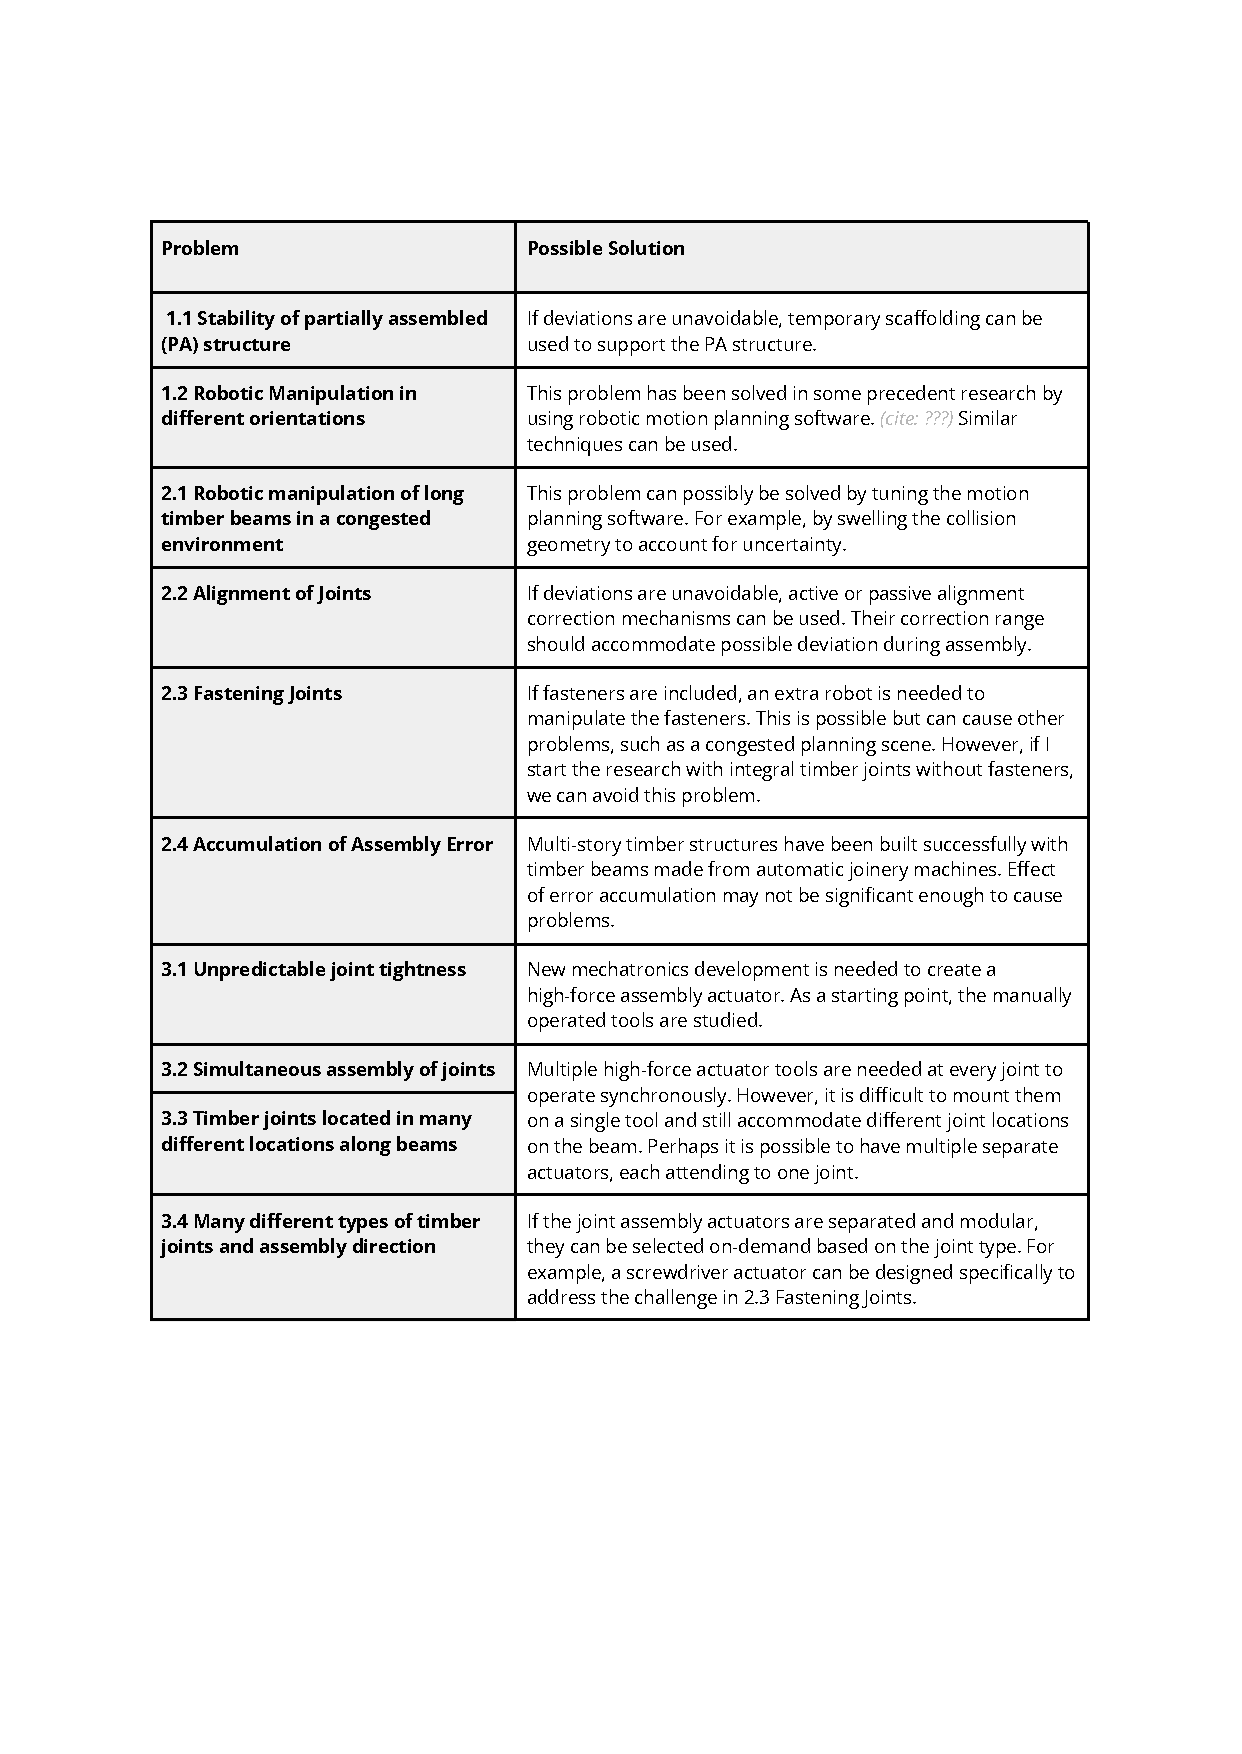
\includegraphics[page=1, trim=25.4mm 60mm 25.4mm 33mm, clip, width=\textwidth]{tables/Tables in Chapter 4.pdf}
    \caption{Author's response to the assembly challenges}
    \label{table:response-to-challenges}
\end{table}

I conducted a survey of tools used by carpenters to applying assembly force for closing joints. The first is a hammer-type tool.\footnote{There are other names for the carpentry hammer, such as mallet, beetle} The striking action of a hammer delivers a short but strong spike of force that momentarily overcome friction to drive joints together. However, it is only effective if a striking surface is available near the joint, as the flexible timber material can absorb the shock. Moreover, hammers are ineffective if the striking direction is upright, as it is difficult to work against gravity. 

The second is a joint-puller-type tool. It often consists of a pair of hooks that can be tightened by a screw or ratcheting mechanism. The hooks can be hammered into the timber or hooked into pre-drilled holes on both sides and pull the joint together. Joint-pullers are particularly useful for pulling liner elements along its length, such as in a splice joint, where a striking surface is not available near the joint. 

The third is a clamp-type tool. It is often used for lap joints where parallel surfaces are easily reachable for clamping. Among different designs, F-shaped clamps are often used because their opening can be quickly adjusted. The joint puller type and the clamp type tools can be used in various orientations regardless of the direction of gravity and they can also be used as a means of temporary support after they are tightened. 

For beams that require the assembly of multiple joints, it is common for multiple workers to actuate the assembly tools synchronously. Because the assembly tools can only apply local forces to each pair of joints, if the assembly motion is not synchronised, the overall beam will deviate from the assembly trajectory (e.g. starts to rotate) and can get stuck due to the jamming effect. This problem is similar to the peg-hole insertion jamming problem studied in robotic assembly. \parencite{dupontJammingWedgingConstrained1994} Therefore, assembly workers need to keep an eye on the overall progress of the entire beam and adjust their actuation speed or hammering force accordingly. 

\subsection{Distributed Robotic Tool (DiRT) Approach}
\label{subsection:exploration-1-distributed-robotic-tool-approach}

From the insights gained from challenges 3.2 to 3.4, it became evident that deploying multiple high-force assembly actuators on each mating joint is a promising approach. Moreover, these actuators should not be fixed together such that it is flexible to position them where the joints are. However, it is challenging to use one robotic arm to hold each end-effector during operation as the number of robots needed may result in congestion near the active beam. Furthermore, this approach is not scalable when working with timber elements that have a large number of joints. 

Therefore, I hypothesised a scenario in which the actuators are attached to and hanging from the Partially Assembled (PA) structure. The attachment and detachment of the tools can therefore be performed one by one, using as few as one robotic arm. After all the actuators are in place, the robotic arm can bring the next piece of timber towards the joints, and perform the assembly with all the actuators exerting force locally at each joint. Because these actuators are no longer tethered to the rest of the robotic system, I called this a “Distributed Robotic Tool” (DiRT) approach. 
This distributed approach does not only address the robot congestion issue but also enhances the scalability and flexibility of the system, making it better suited for timber assembly tasks with varying levels of complexity. The modularity of distributed tools allows for the development of different tools tailored to different joint types and assembly requirements. The system can intelligently select the appropriate tool based on the design of a structure, joint types, and joint angles. This adaptability ensures that the DiRT approach can effectively address a wide range of timber frame structures.

\subsection{Scope for Initial Exploration Round}
\label{subsection:exploration-1-scope-for-initial-exploration-round}

Because the design of a DiRT assembly tool is specific to the joint type, I had to make a decision on which joint type to be developed first. Among the popular types of timber joints used in timber frame structures, I decided to start the investigation with lap joints. This is because lap joints are the most versatile type of joints that can be used to join many structural members. For details, please see \noseeref{subsection:exploration-1-lap-joint-classification-by-assembly-direction} regarding the definition of Lap Joints used in this thesis and their versatility.

\begin{figure}
    \centering
    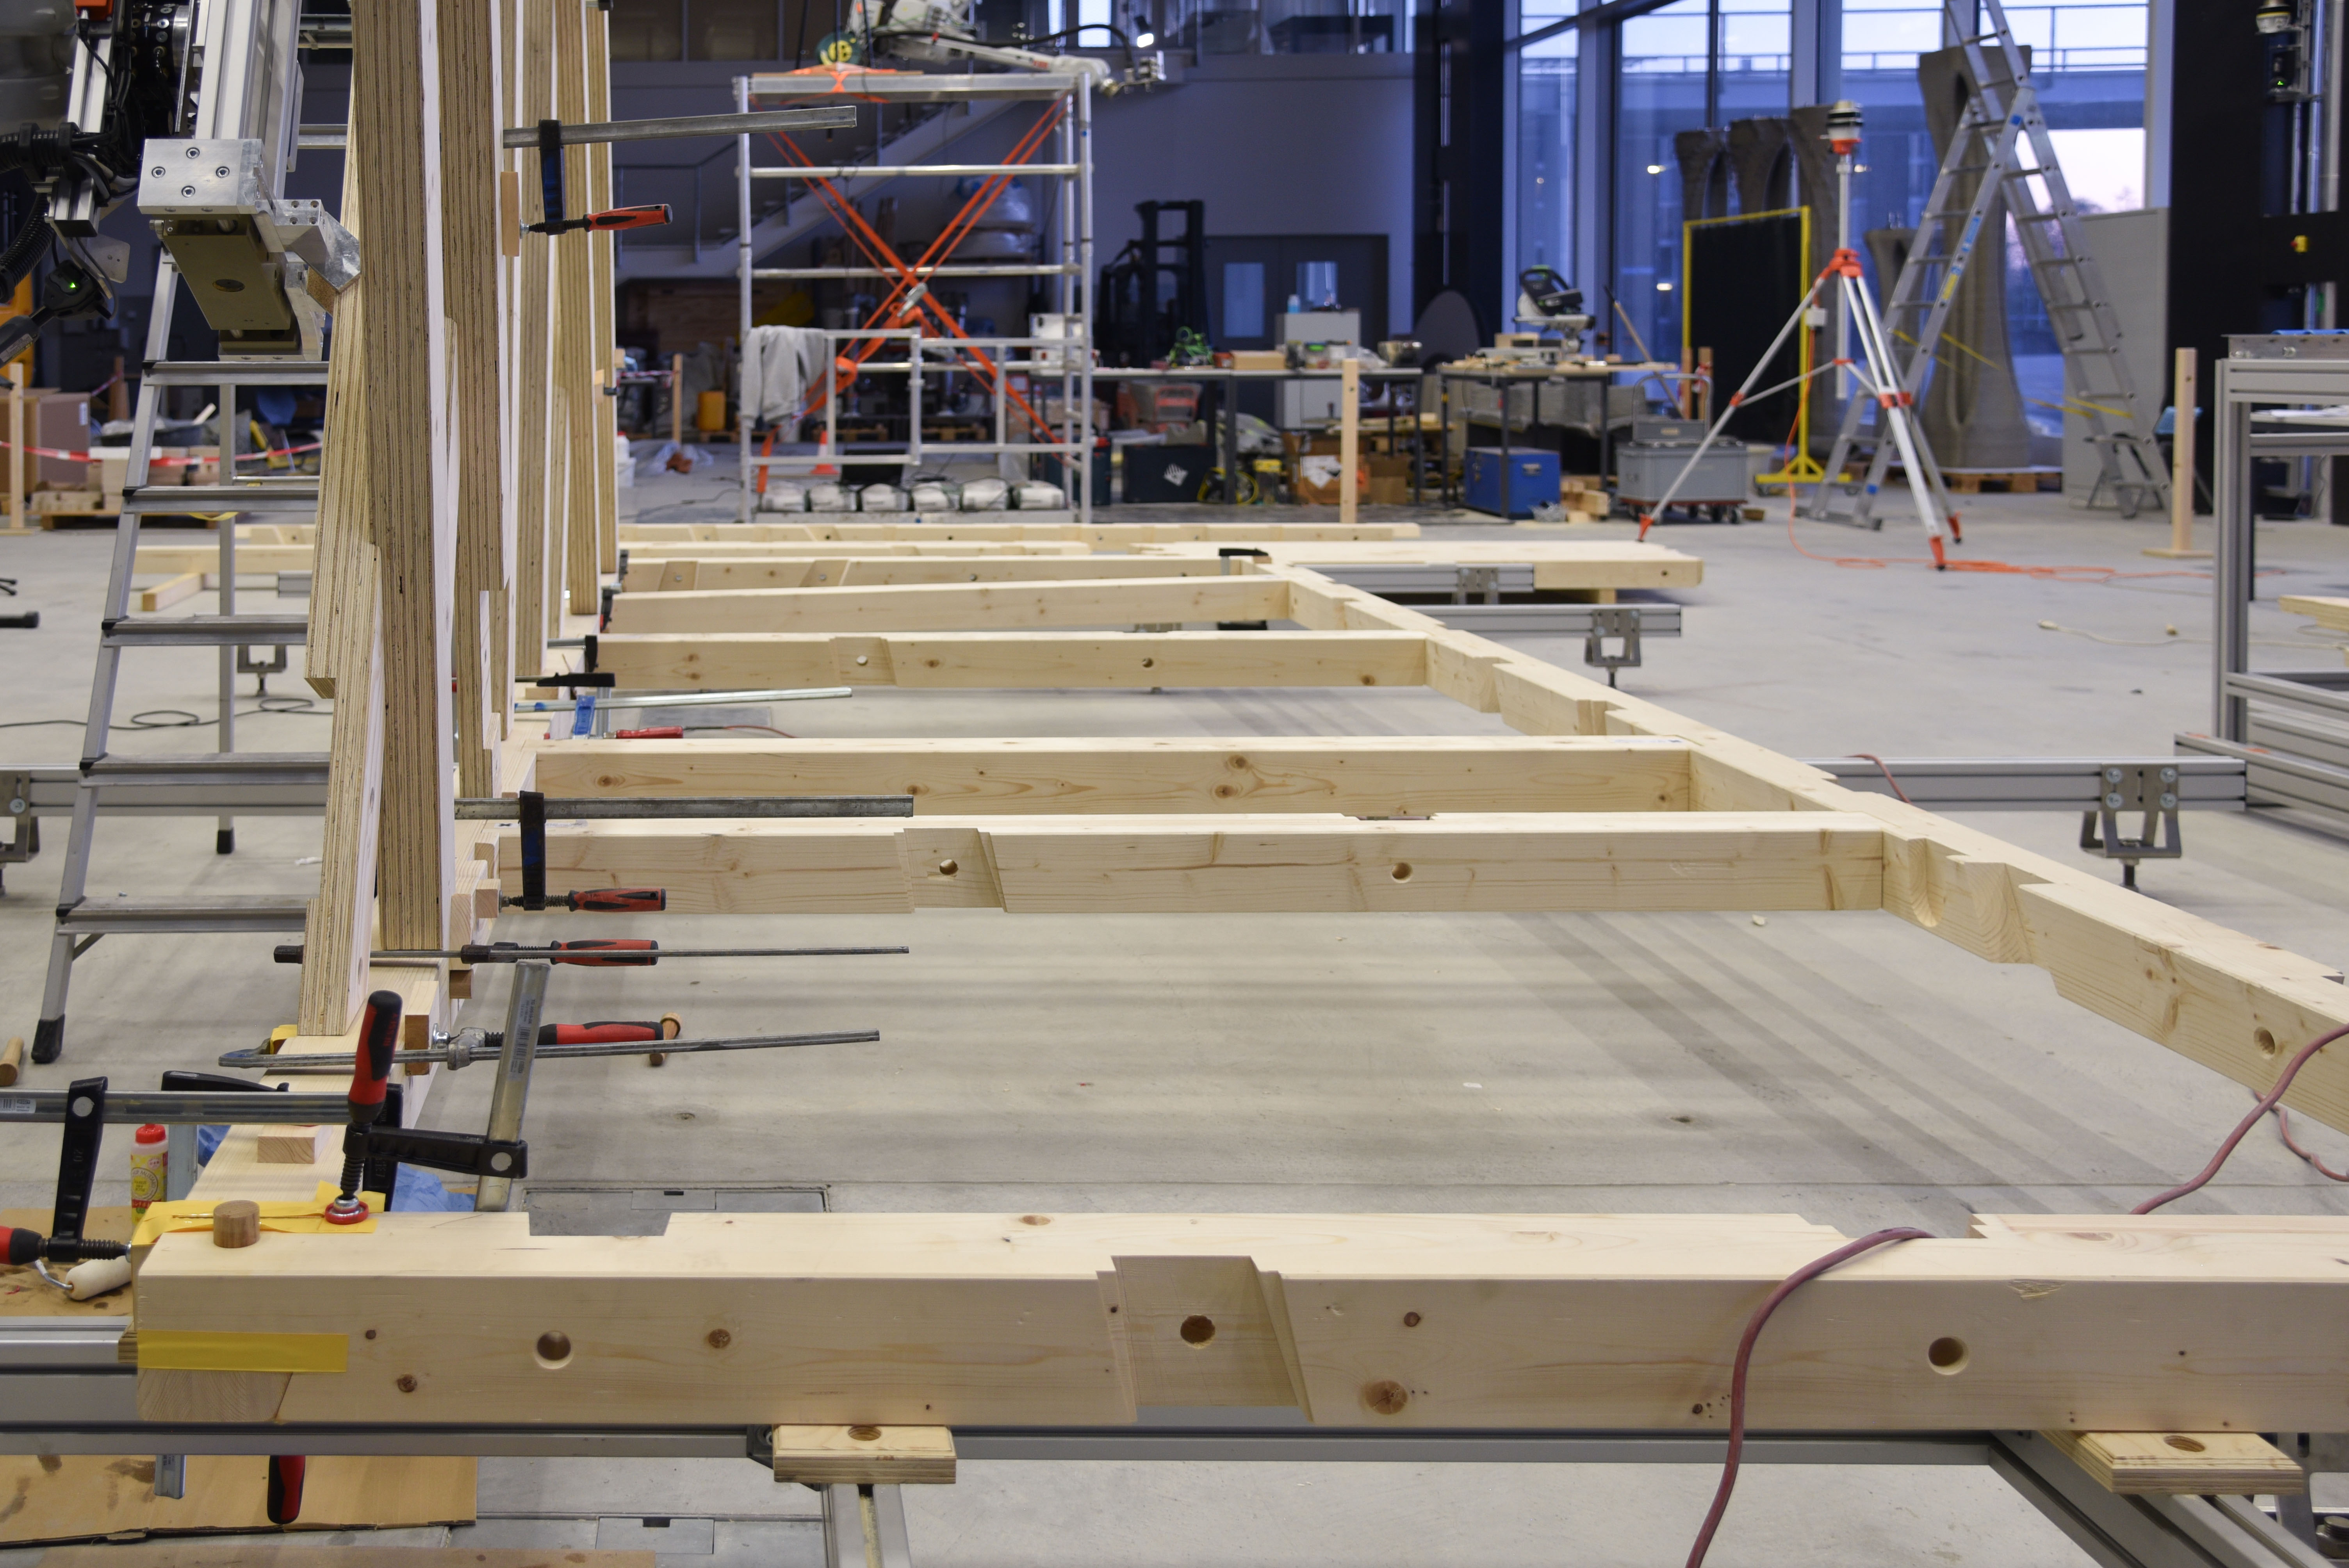
\includegraphics[width=0.99\textwidth]{images/04-1+2/clamp-inspiration.jpeg}
    \caption{Example of carpentry clamps used in timber construction.}
    \label{fig:clamp-inspiration}
\end{figure}

Based on a review of the manual tools used for assembling lap joints, I have shortlisted two promising actuator arrangements. The first arrangement is a clamping mechanism similar to carpentry clamps, which apply a compression force to the outside of the lap joints (see Figure \ref{fig:clamp-inspiration}). The second arrangement is a screwing mechanism that uses a screw to pull the two sides of a joint together. I decided to start the development with the clamping mechanism because it is mechanically simpler. In later exploration rounds, the screwing mechanism was also explored \seeref{section:exploration-4-goal}.

In this exploration round, the focus is to:
\begin{itemize}
    \item Validate the robotic clamping streategy for the assembly of lap joints, starting with an orthogonal lap joint.
    \item Explore streategies for hanging a robotic clamping tool on the timber structure.
\end{itemize}

This is achieved through a series of mechatronics development to create a robotic clamp. On the other hand, other essential features of DiRT operations such as remote control, battery packs and wireless communication systems are postponed to later development.
In order to simplify initial development, I decided to pick a timber size standard of \textbf{100x100mm square profile}. This is selected after careful consideration to fulfil the following criteria:
\begin{itemize}[nosep]
    \item A profile size commonly available in Switzerland to facilitate demonstrations and experiments.
    \item A profile big enough to be strong structurally and can be used as beams, columns and bracings.
    \item A profile small enough such that the robotic arm in the lab (with its limited payload) can manipulate a long beam.
\end{itemize}

For the timber species and processing, I chose \textbf{glue-laminated spruce} as the intended material because it is one of the most commonly used construction timber in Switzerland. The timber material used in this thesis has the following properties:

\begin{itemize}[nosep]
    \item Strength class: GL24h 
    \item Appearance class: N
    \item Lamination composition: Duo or Trio
    \item Gluing standard: DIN EN 14 080 
    \item Moisture Content 13\% ± 3\%
    \item Nominal Density 460kg/m3
\end{itemize}

\subsection{DiRT Clamping Assembly Process Task List (Version 1)}
\label{subsection:exploration-1-dirt-clamping-assembly-process-task-list-v1}

The working hypothesis of the Distributed Robotic Tool (DiRT) System for timber frame assembly consists of two main hardware components:
\begin{itemize}[nosep]
    \item A set of distributed robotic clamps (the “clamps”), each of which $\cdots$
    \begin{itemize}
        \item Can be attached to the joint area
        \item Can perform a clamping action on lap joints
        \item Can be operated wirelessly and synchronously
    \end{itemize}
    \item A robotic arm mounted on gantry axes (the “robot”) that $\cdots$
    \begin{itemize}
        \item Can attach clamps on the Partially Assembled (PA) structure
        \item Can bring a timber beam to the clamps
        \item Can move the timber beam together while the clamps are clamping
        \item Can retrieve the clamps after they are finished
    \end{itemize}
\end{itemize}

Their operation is based on a repetitive cycle for every beam to be assembled. Table \ref{table:list-of-assembly-tasks} describes a list of tasks according to their order of operation and a shortened name for referring to them later in this thesis.

\begin{table}[H]
    \includegraphics[page=2, trim=25.4mm 100mm 25.4mm 33mm, clip, width=\textwidth]{tables/Tables in Chapter 4.pdf}
    \caption{List of tasks in a repetitive cycle for assembling timber beams}
    \label{table:list-of-assembly-tasks}
\end{table}

% \clearpage

\begin{figure}[p]
    \centering
    \begin{subfigure}[b]{0.49\textwidth}
        \centering
        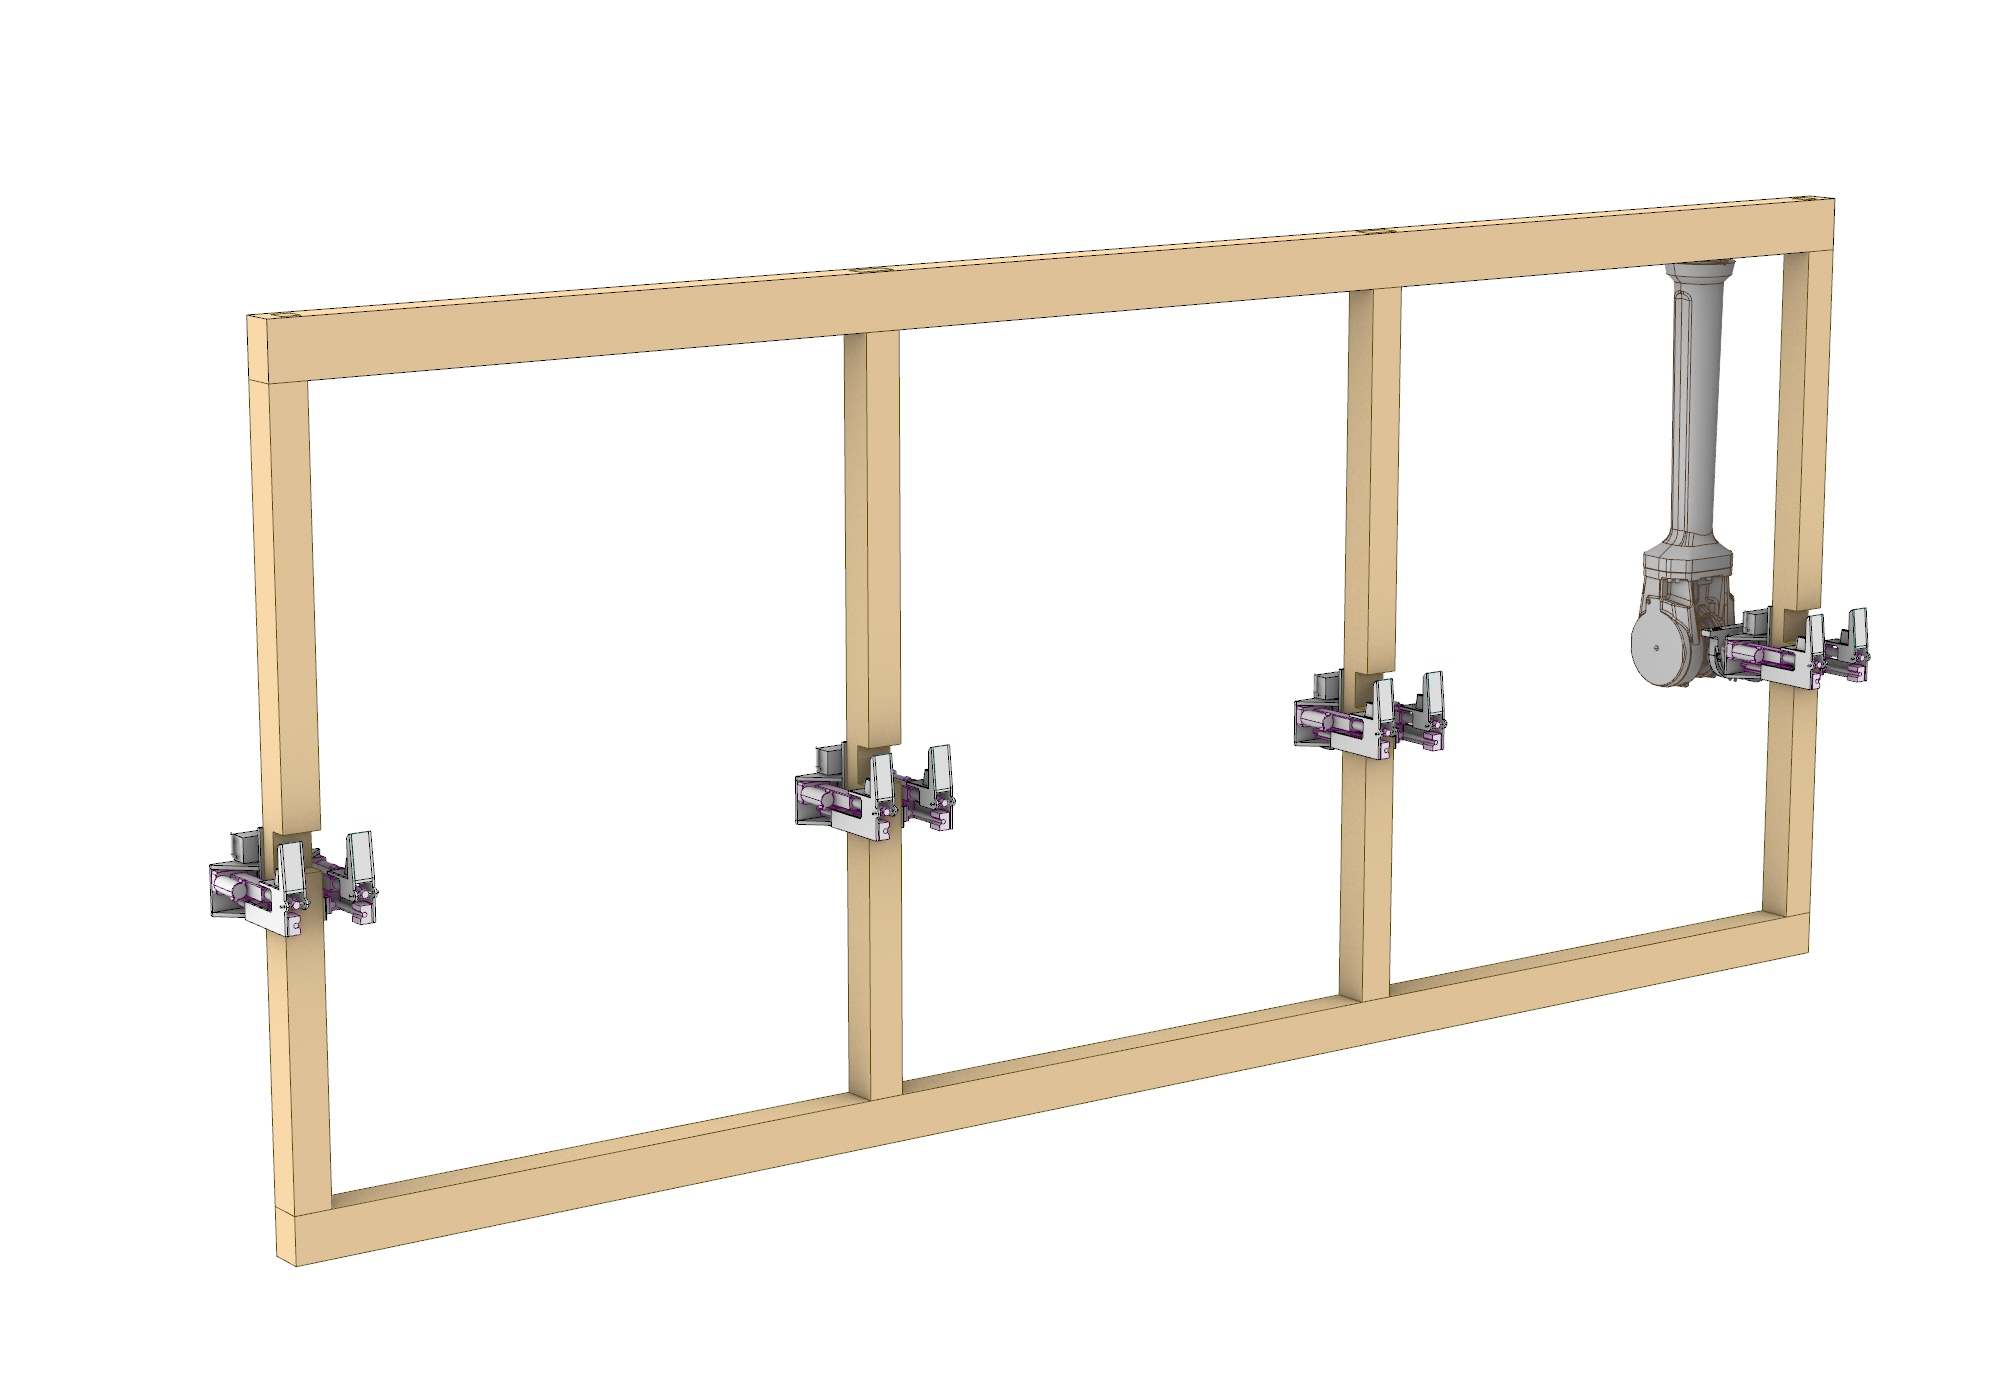
\includegraphics[width=\textwidth]{images/04-1+2/Multiple_4.jpg}
        \caption{The moment after the fourth {\tt PlaceClampToStructure}}
        \label{fig:fig:beam-assembly-step1}
    \end{subfigure}
    \hfill
    \begin{subfigure}[b]{0.49\textwidth}
        \centering
        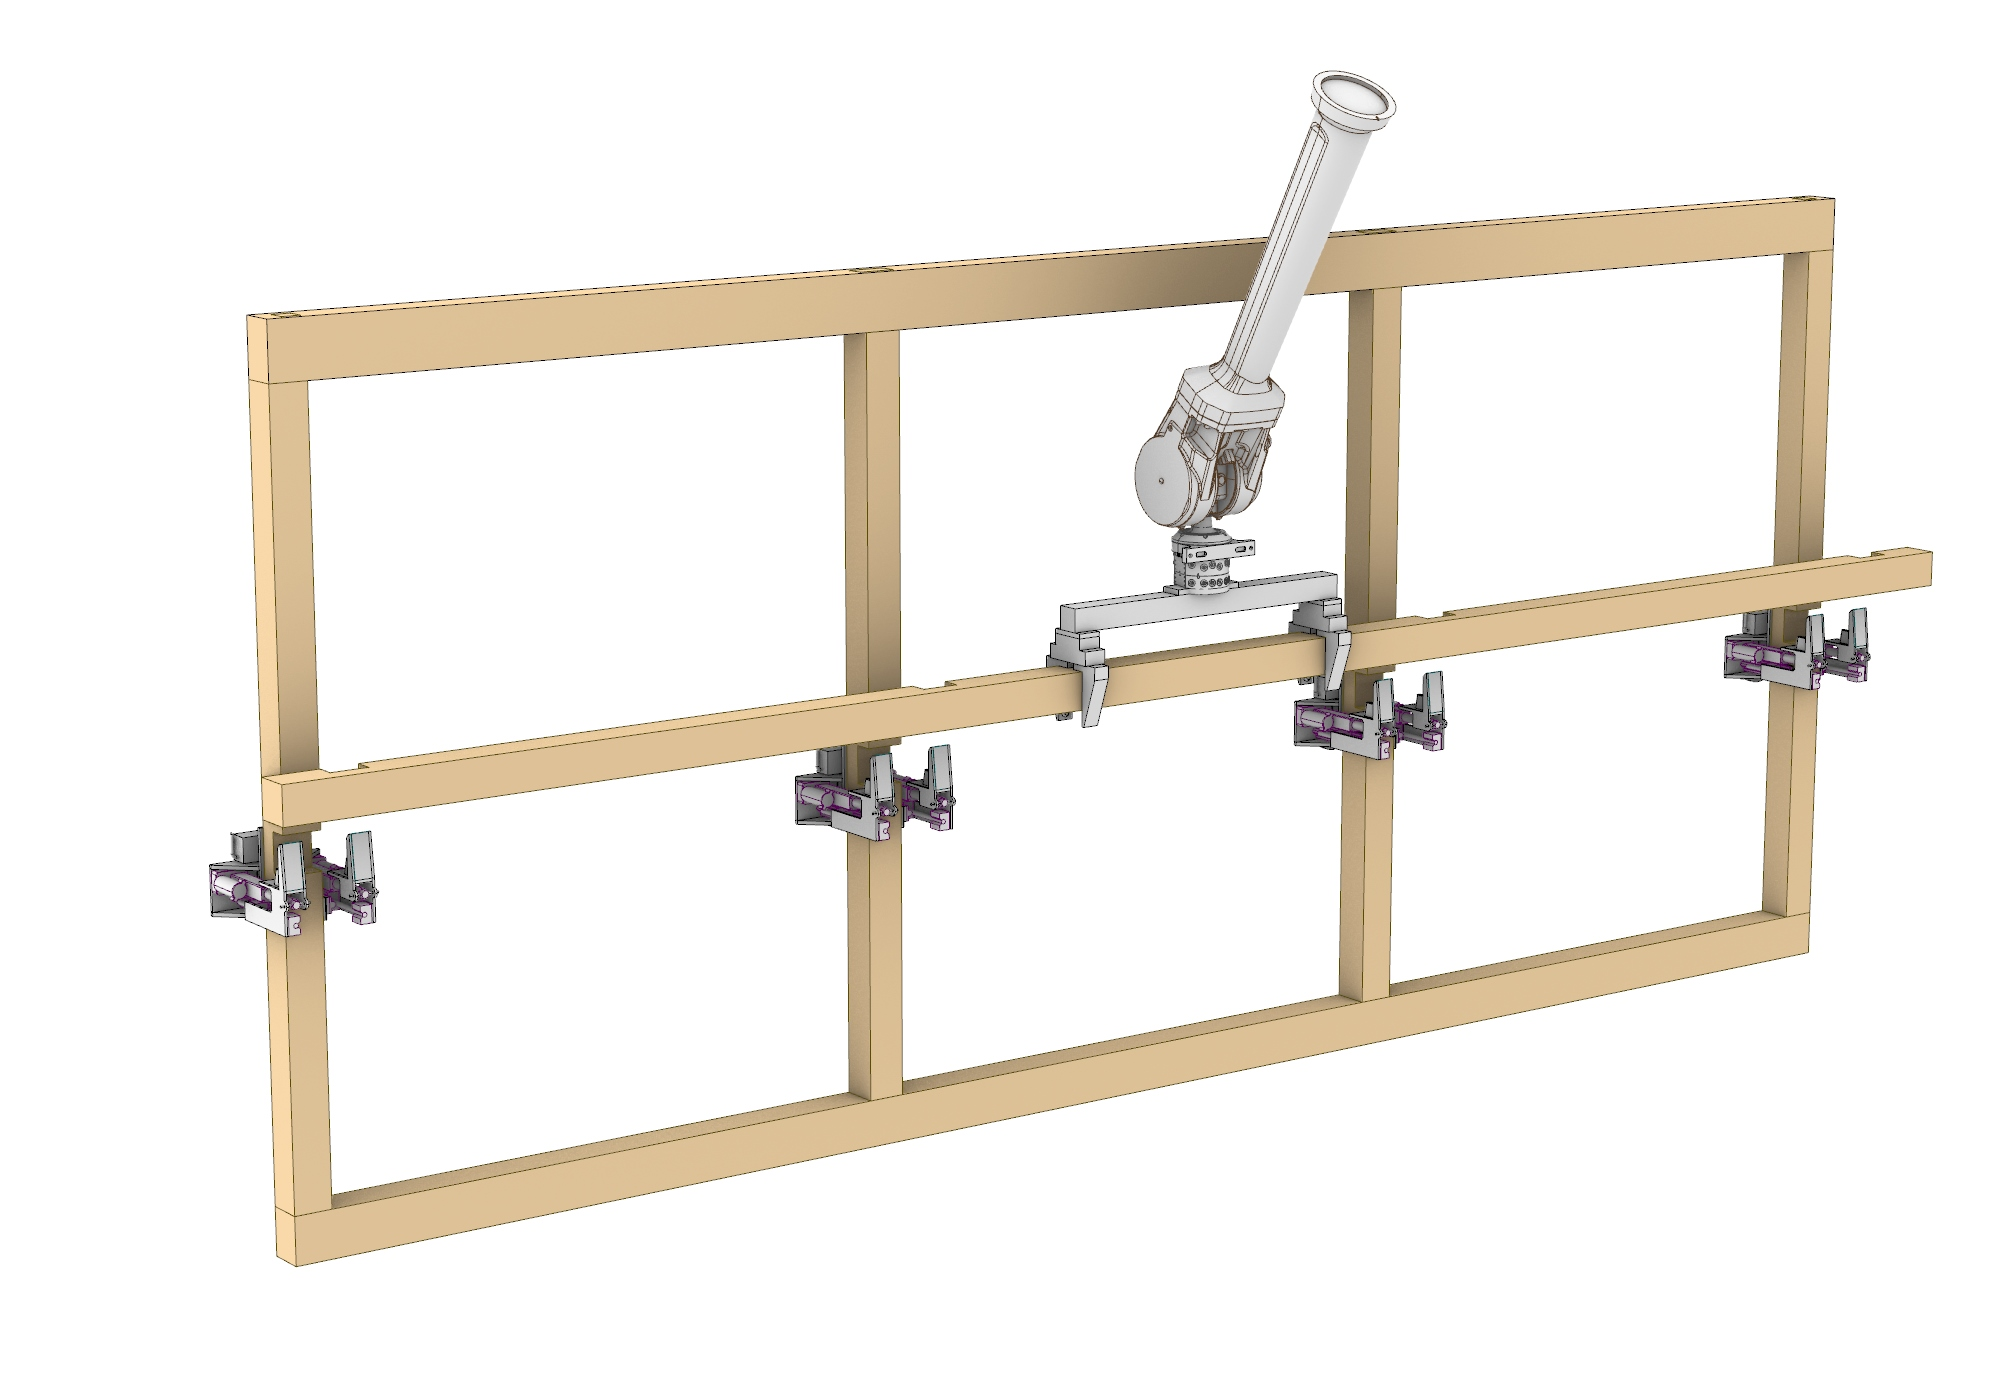
\includegraphics[width=\textwidth]{images/04-1+2/Multiple_5.jpg}
        \caption{The moment after \codett{BeamTransfer} but before \codett{ PlaceBeamInClamp}}
        \label{fig:fig:beam-assembly-step2}
    \end{subfigure}
    \vskip\baselineskip % Next row
    \begin{subfigure}[b]{0.49\textwidth}
        \centering
        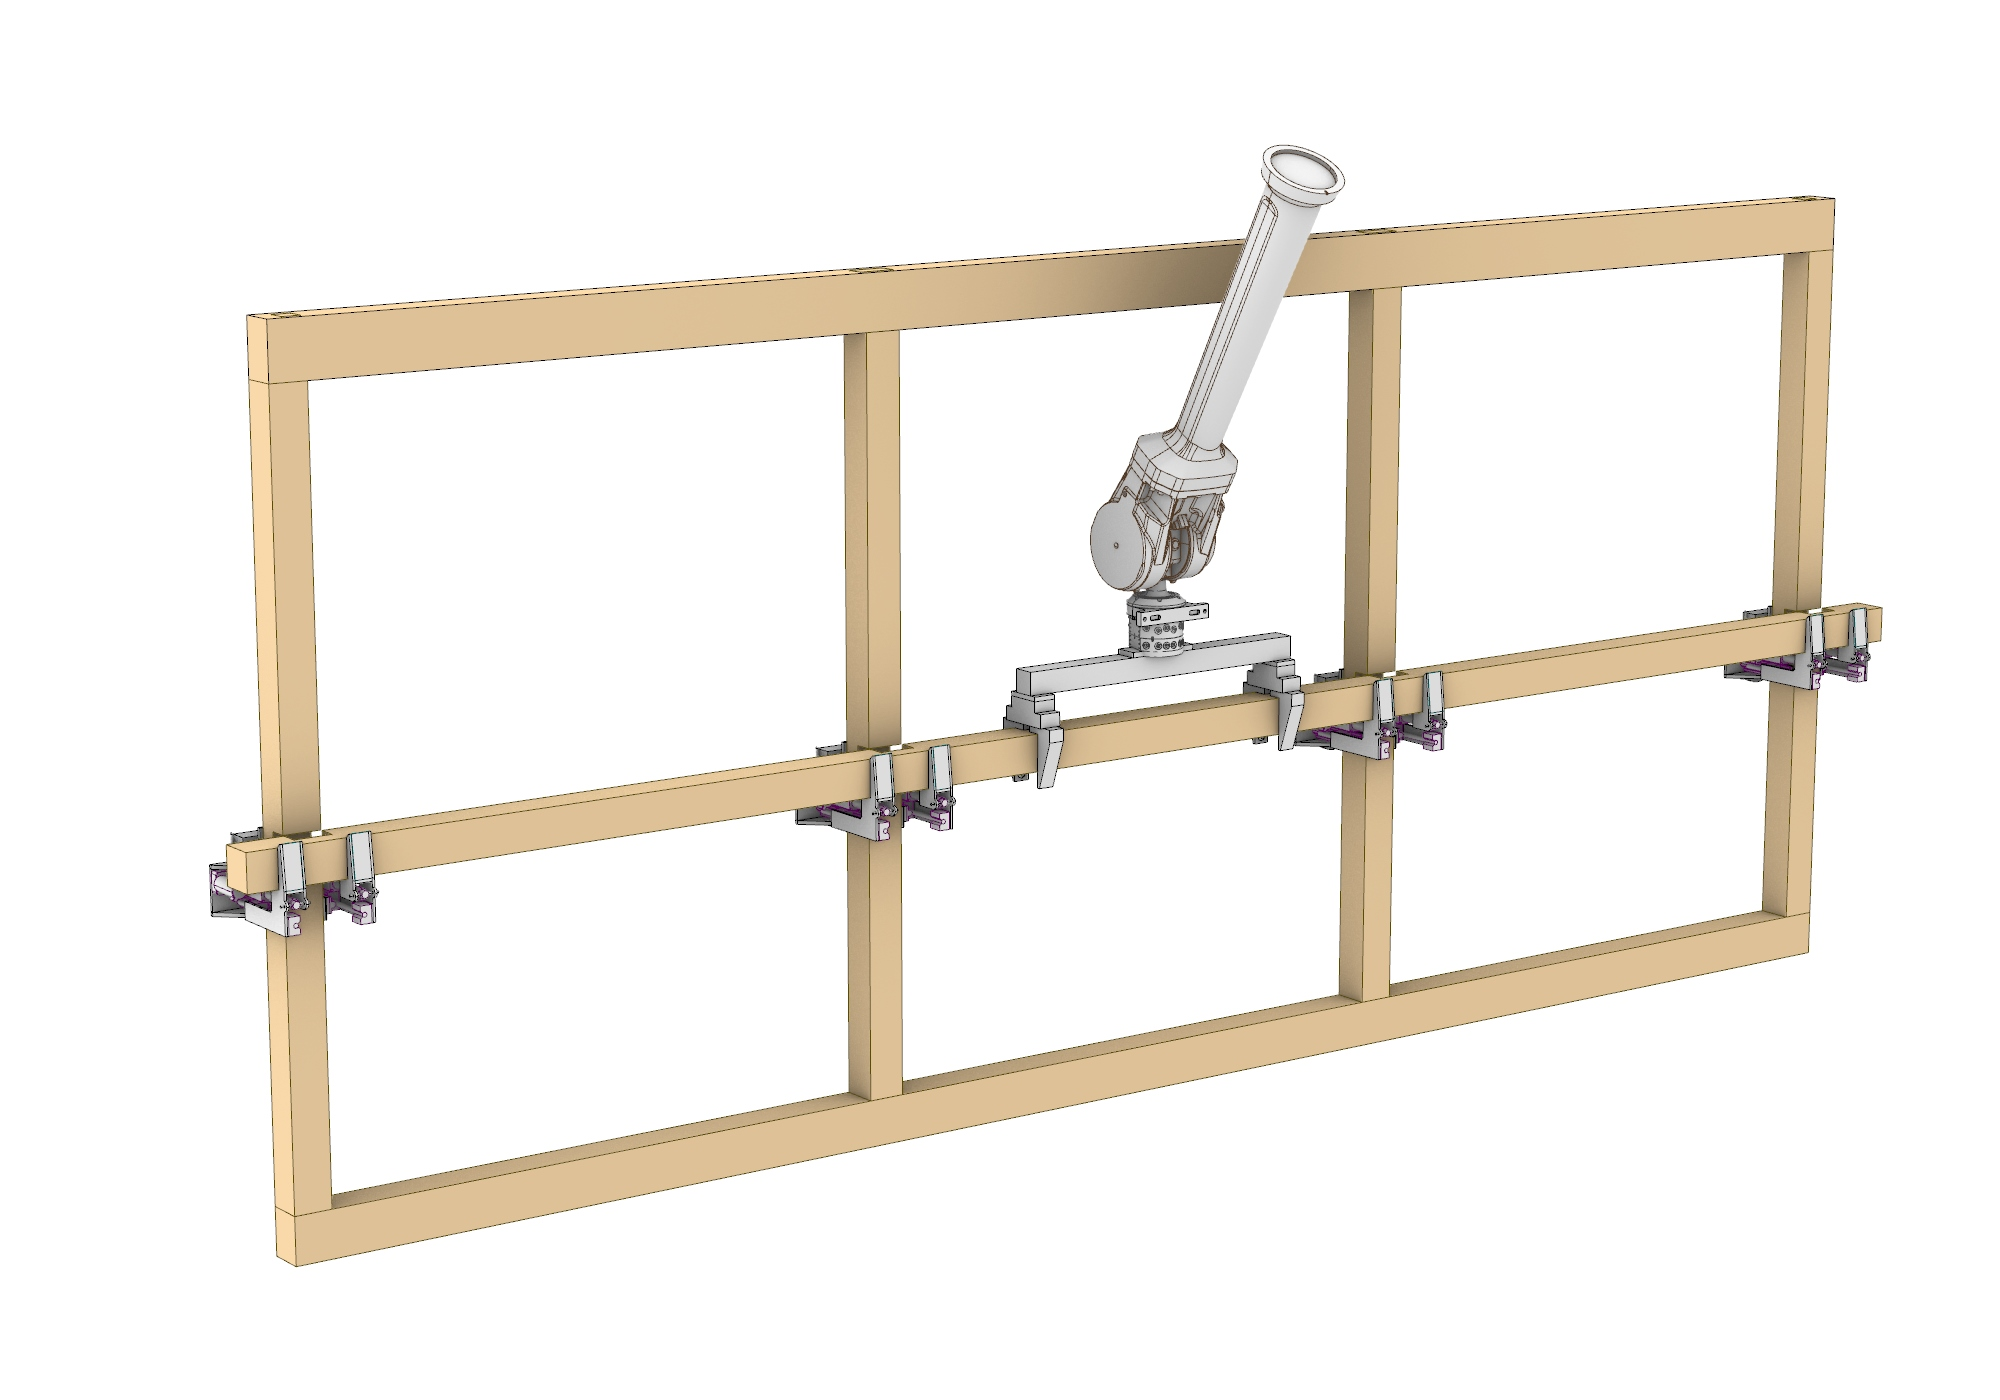
\includegraphics[width=\textwidth]{images/04-1+2/Multiple_7.jpg}
        \caption{The moment after {\tt PlaceBeamInClamp}}
        \label{fig:fig:beam-assembly-step3}
    \end{subfigure}
    \hfill
    \begin{subfigure}[b]{0.49\textwidth}
        \centering
        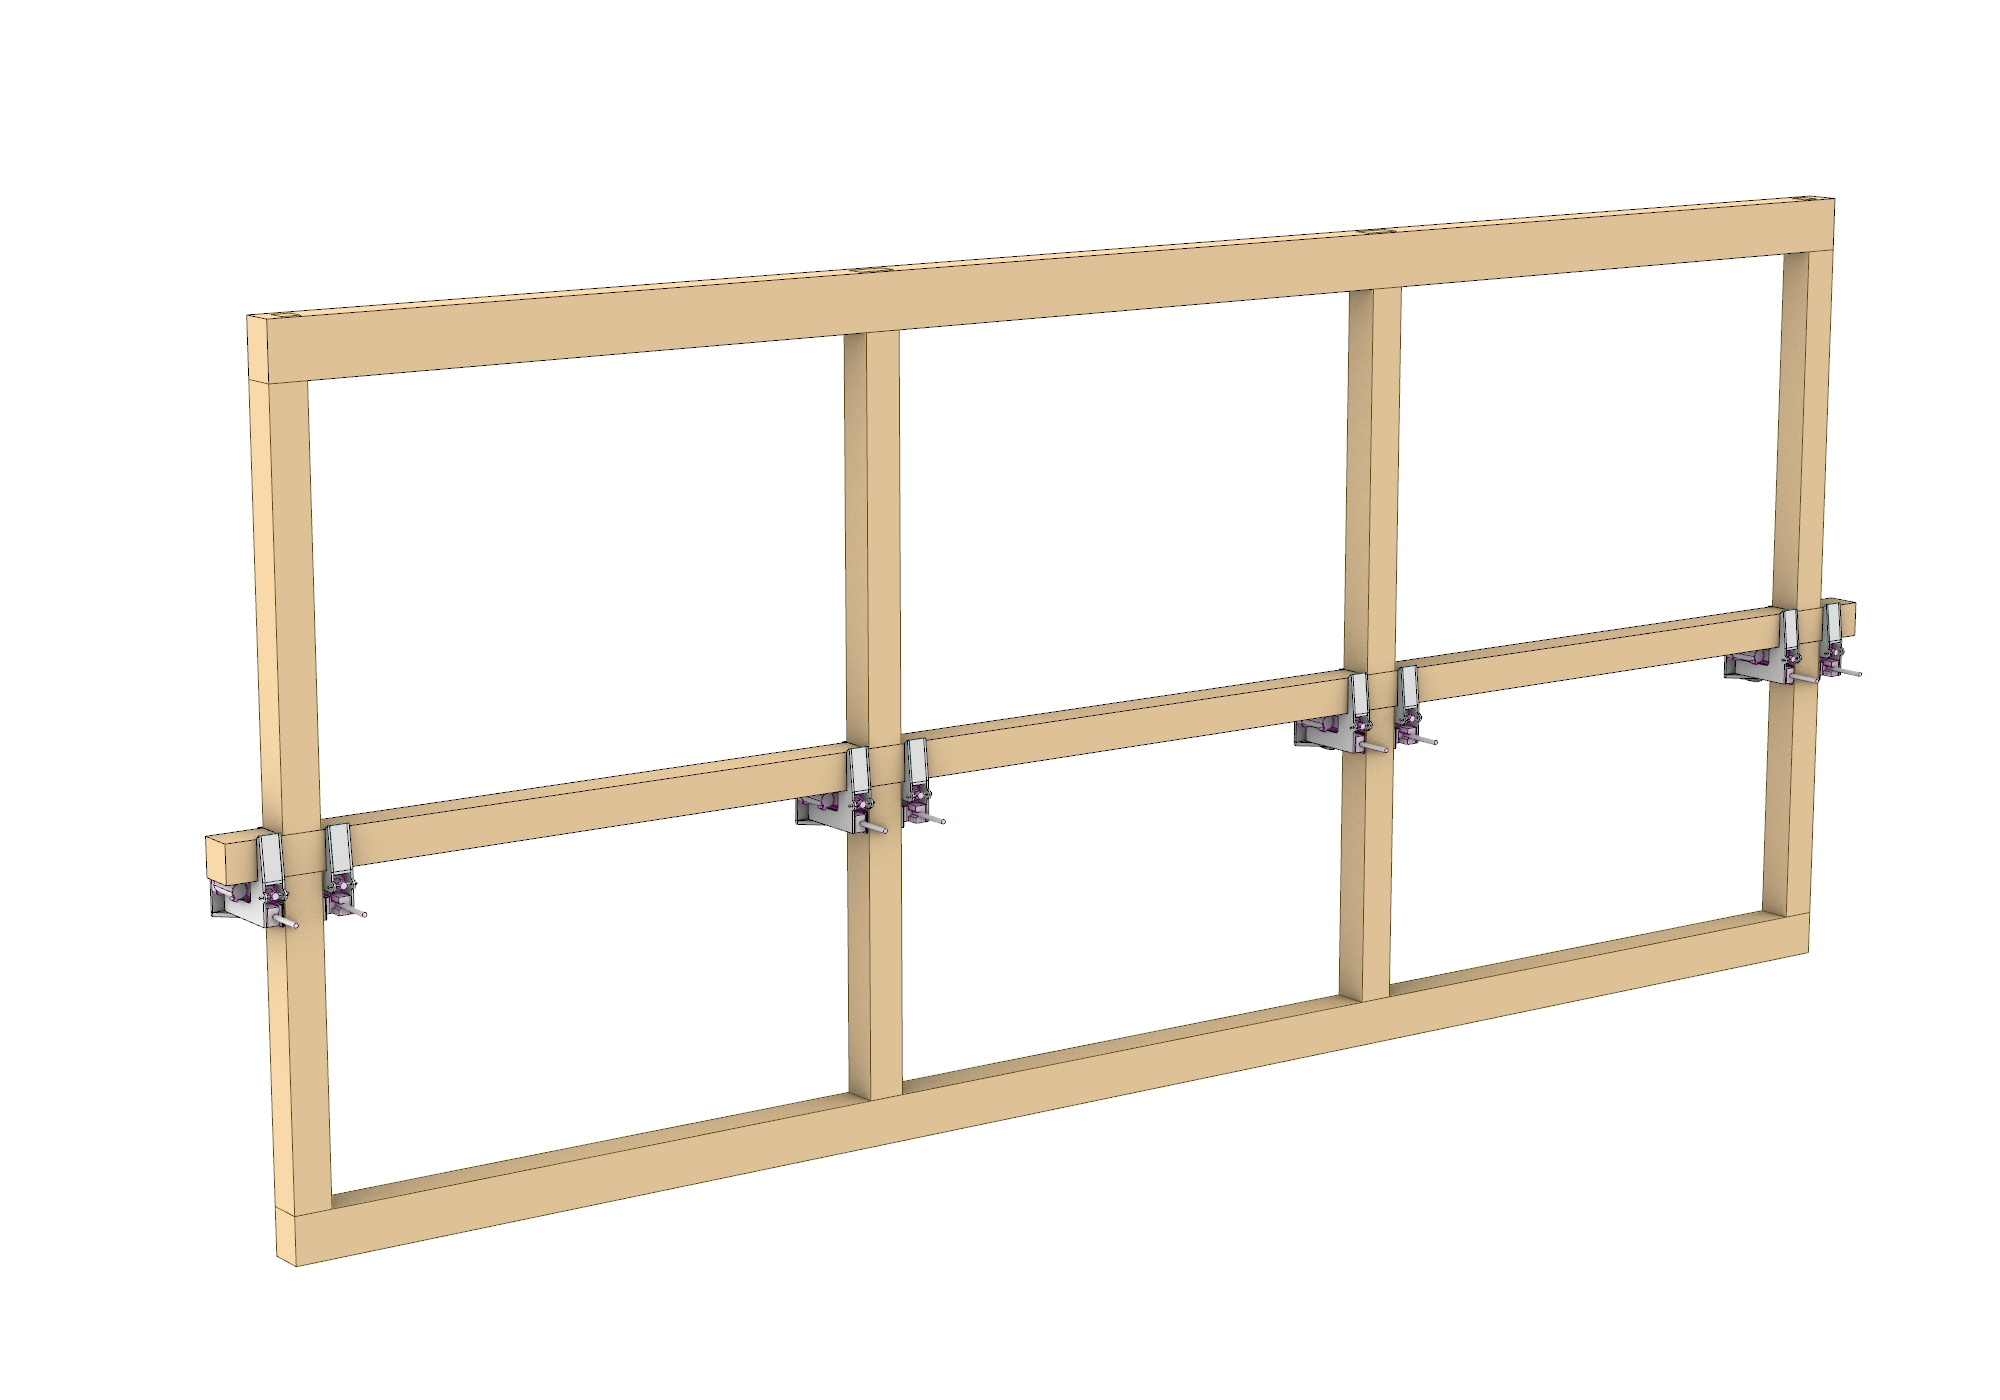
\includegraphics[width=\textwidth]{images/04-1+2/Multiple_10.jpg}
        \caption{The moment after {\tt ClampSyncAssembly}}
        \label{fig:fig:beam-assembly-step4}
    \end{subfigure}
        \vskip\baselineskip % Next row
    \begin{subfigure}[b]{0.49\textwidth}
        \centering
        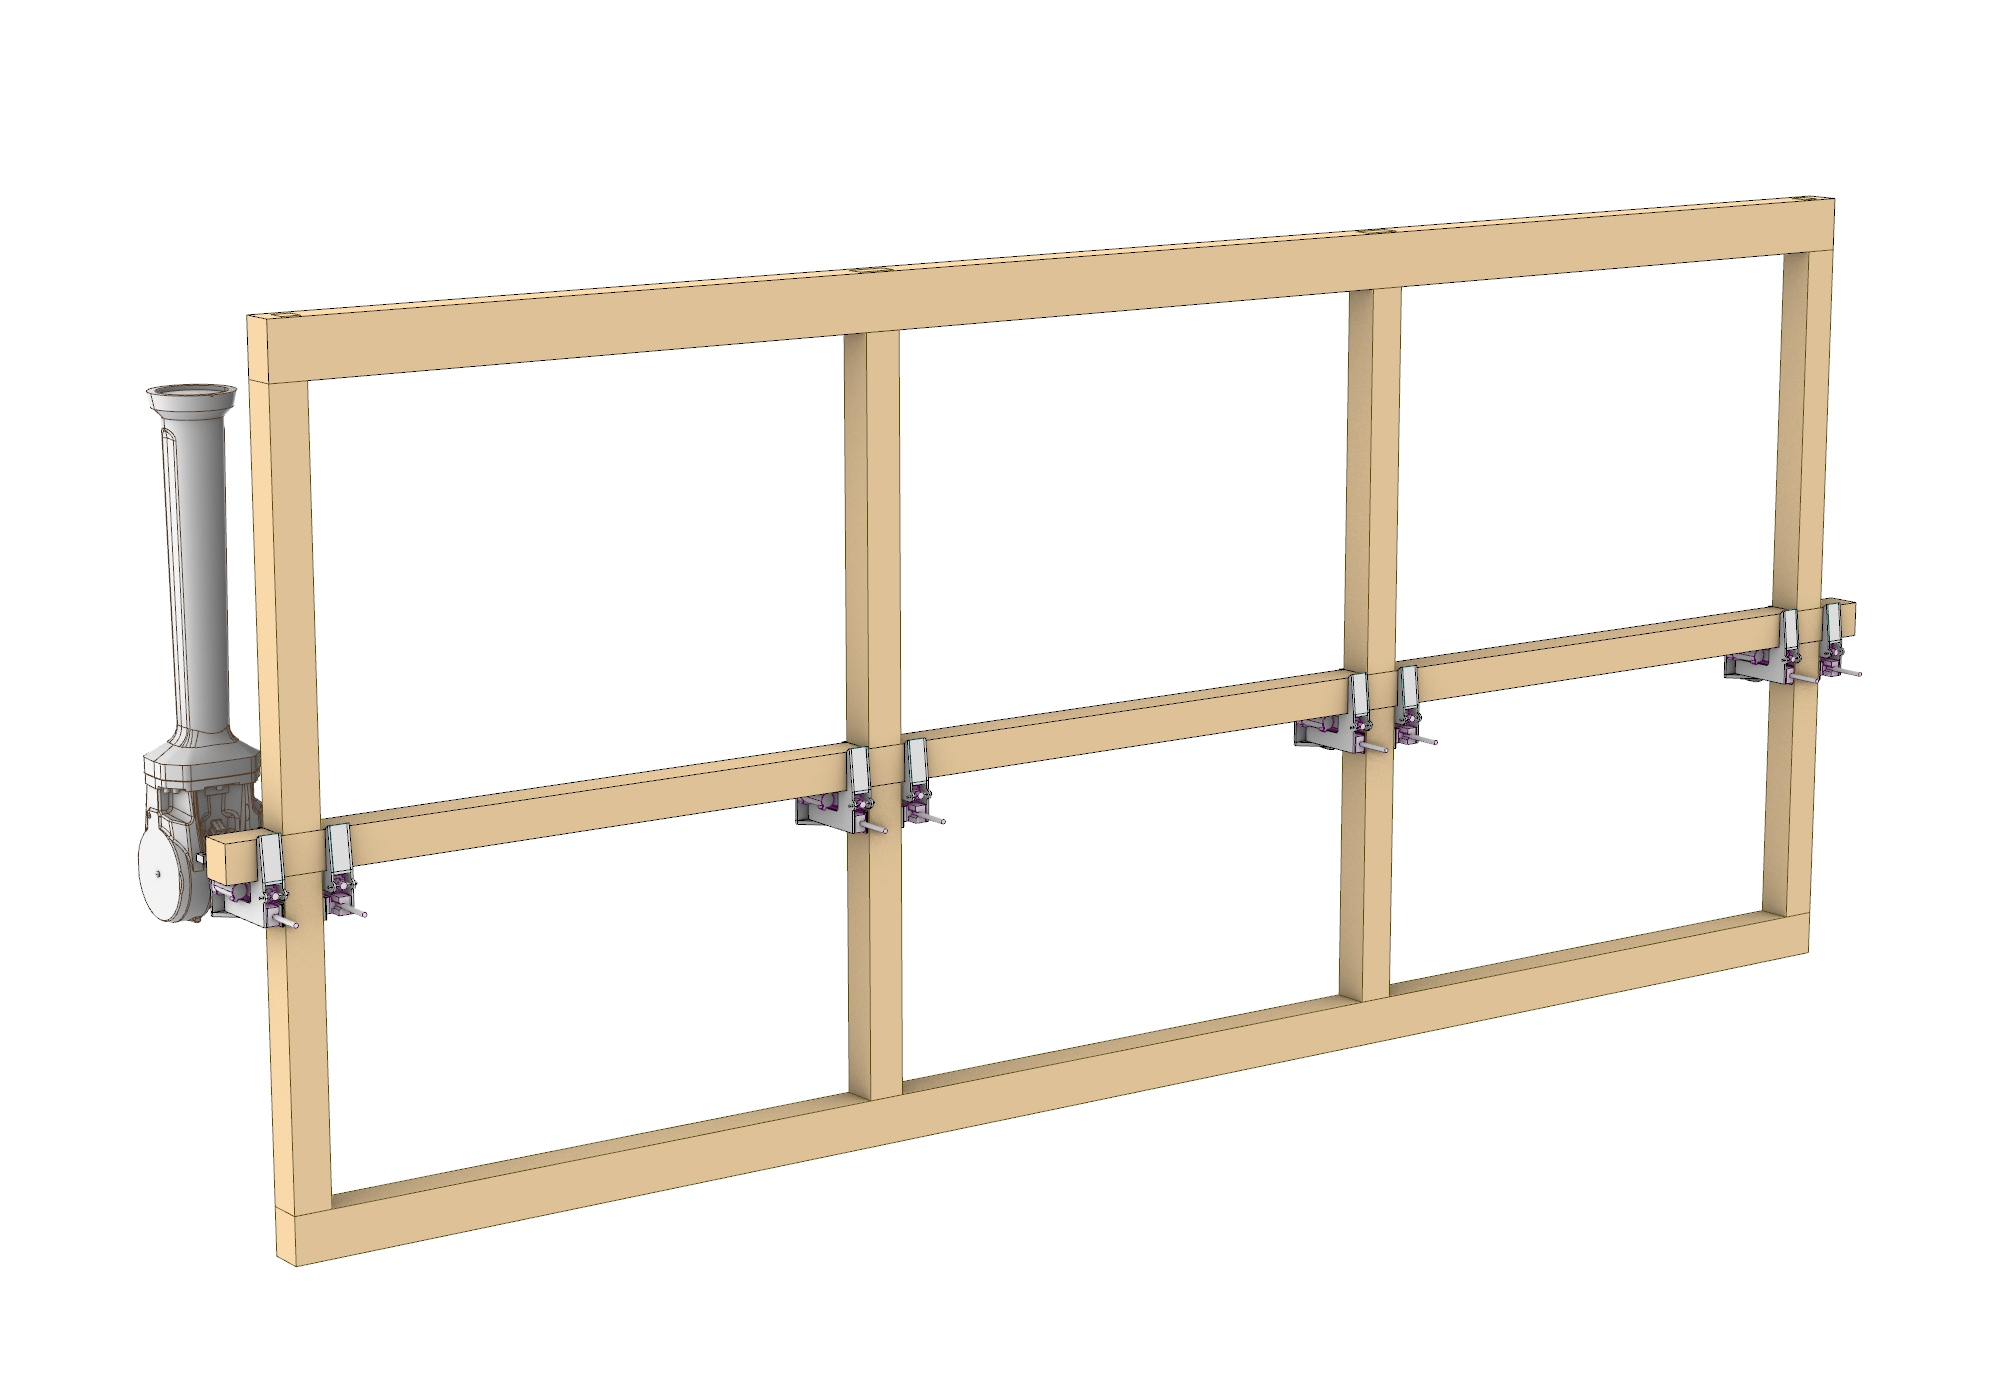
\includegraphics[width=\textwidth]{images/04-1+2/Multiple_11.jpg}
        \caption{The moment before the first {\tt PickClampFromStructure}}
        \label{fig:fig:beam-assembly-step5}
    \end{subfigure}
    \hfill
    \begin{subfigure}[b]{0.49\textwidth}
        \centering
        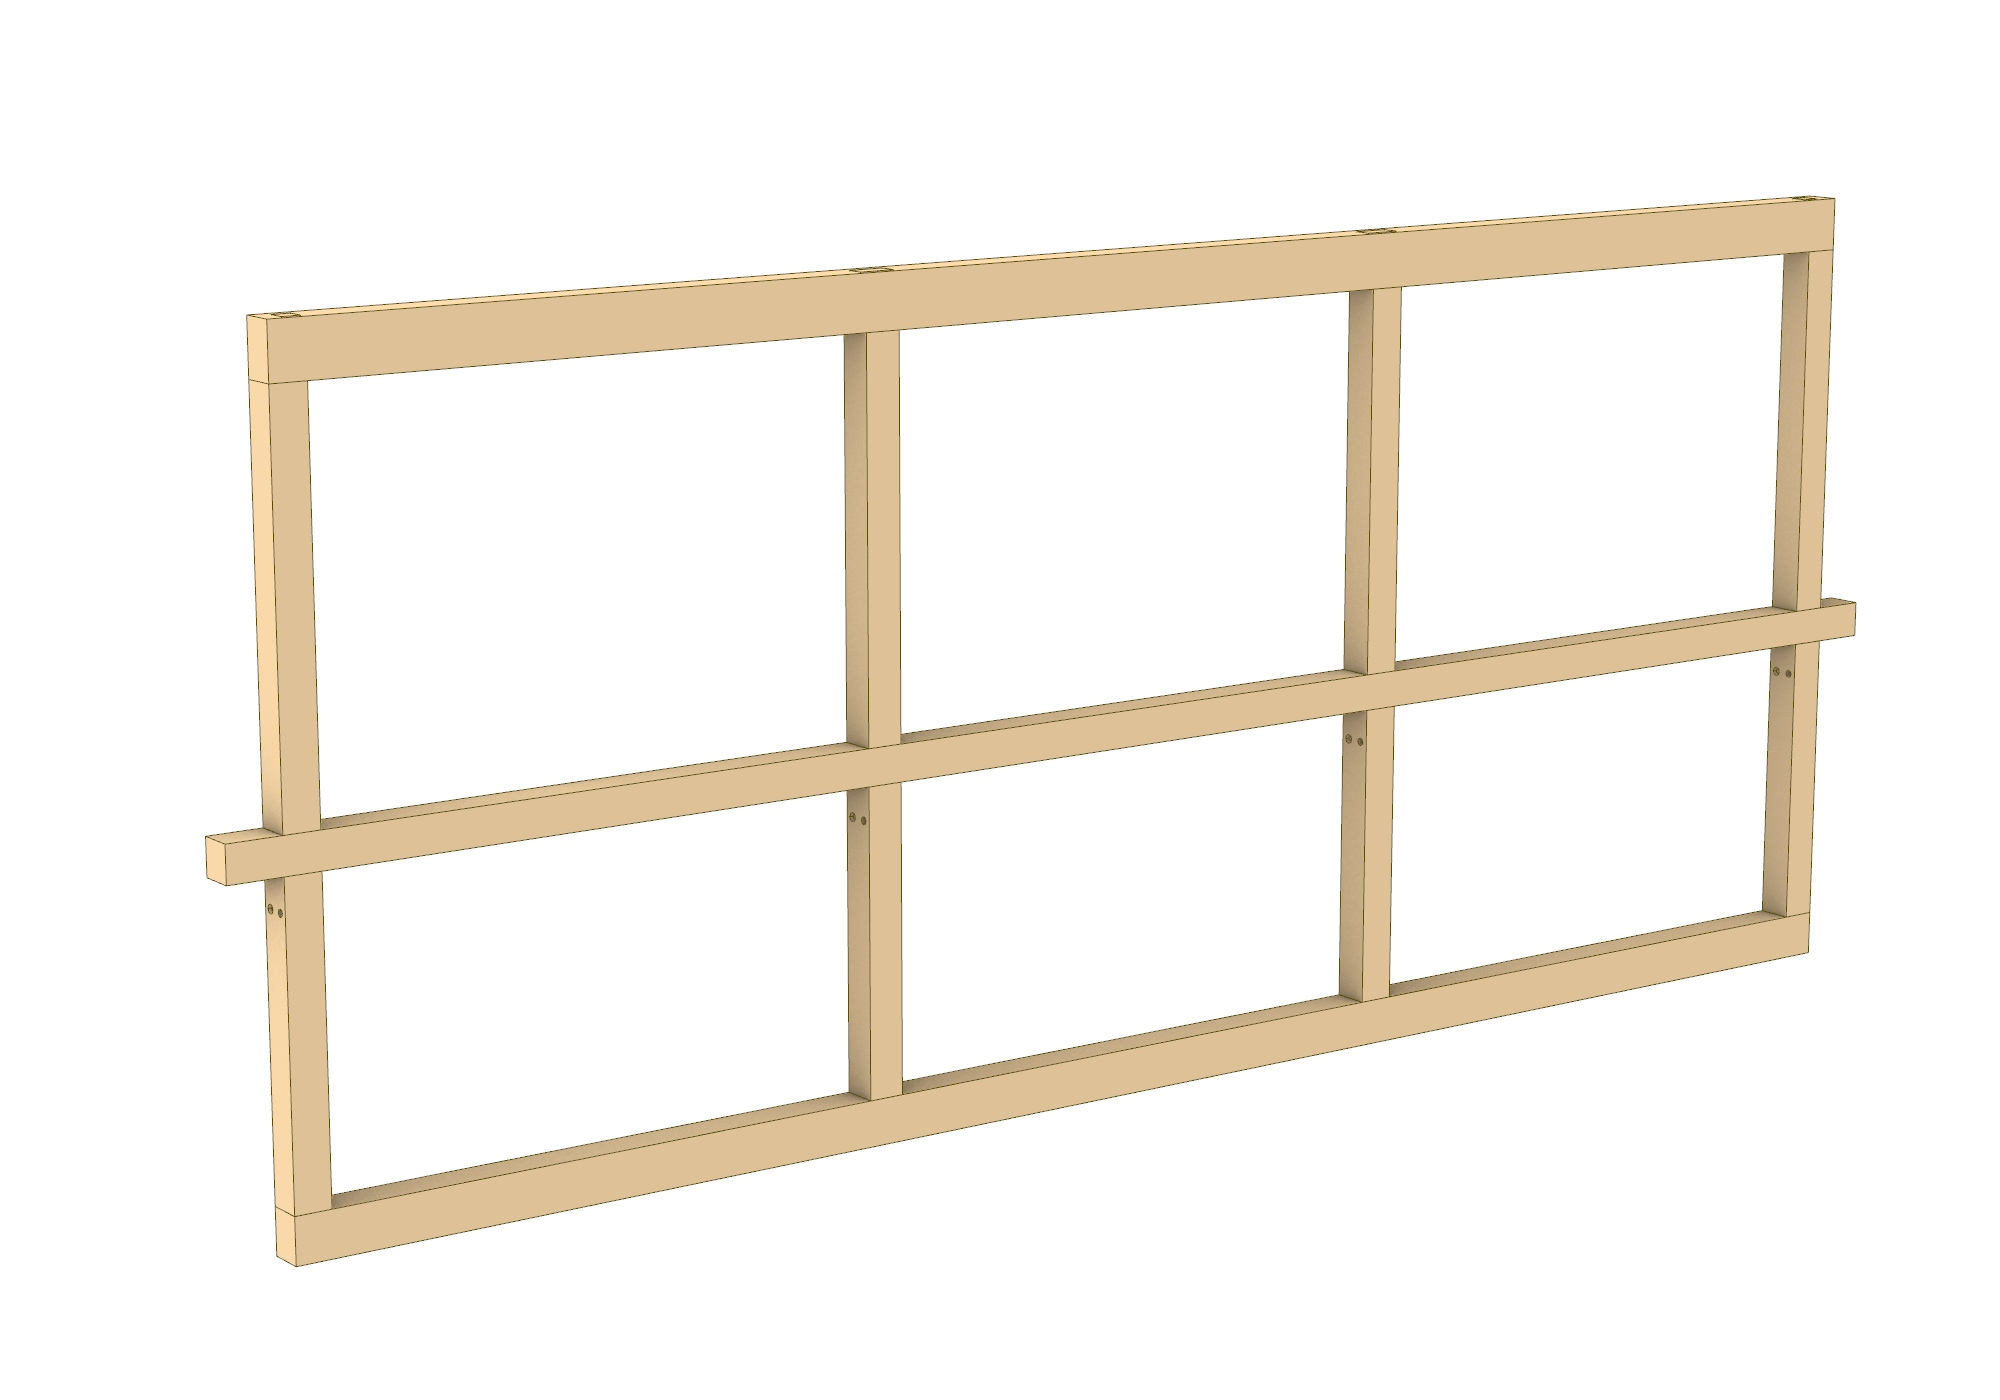
\includegraphics[width=\textwidth]{images/04-1+2/Multiple_15.jpg}
        \caption{The moment at the end of the cycle, after the last {\tt PlaceClampToStorage}}
        \label{fig:fig:beam-assembly-step6}
    \end{subfigure}
    \caption[Diagrams illustrating the assembly steps of a horizontal beam]
    {Diagrams illustrating the assembly steps of a horizontal beam (refer to Table \ref{table:list-of-assembly-tasks} for the description of each step)}
    \label{fig:beam-assembly-six-moments}
\end{figure}

\FloatBarrier

Figure \ref{fig:beam-assembly-six-moments} illustrates the assembly process of a horizontal beam with four simultaneous mating joints. In this initial working hypothesis, the system requires manually assembling the first few columns to the ground before the subsequent process can become fully automatic. At this point, I have not considered how to assemble non-vertical elements. However, this became clear at the end of this exploration round \seeref{subsection:exploration-1-beam-support-needed-during-clamping}.

% \clearpage

\section{Background}
\label{section:exploration-1-background}

\subsection{Lap Joint Classification by Assembly Direction}
\label{subsection:exploration-1-lap-joint-classification-by-assembly-direction}

Timber frame buildings utilize a variety of joints to connect structural elements and create a stable, load-bearing framework. Various categorisation methods have been developed to group them based on their characteristics, functions, or cultural background \seeref{subsection:introduction-defining-characteristics}. As the primary objective of this thesis is to investigate the assembly process of timber frame structures, I adopted a classification method that focuses on the assembly direction of the joints, because it is closely related to the kinematics of the assembly tools.

Lap joints, mortise and tenon joints, and splice joints are three common types of joints found in timber frame construction, each with different assembly directions in relation to the neighbouring elements' arrangements. This thesis focus on the assembly of lap joints, as they represent a straightforward and widely used connection method in timber frame construction. 

Lap joints are formed by overlapping two pieces of timber, with one piece lying on top of the other. The overlapping sections are typically cut to half the thickness of the timber, creating a flush surface.\footnote{Note that in some classifications \parencite{seikeArtJapaneseJoinery1977}, lap joints are not necessarily planar or assembled perpendicular to the flush face. However, this narrower definition simplified the initial development.} Lap joints are widely used in timber frame construction due to their versatility and ability to transfer loads between connected elements effectively. These joints are relatively simple to assemble, as they involve linear assembly motion that is perpendicular to the flush surface. 

Figure \ref{fig:common-joints-crosslap} and \ref{fig:common-joints-teelap} shows cross-shape and tee-shape lap joint, both conform to the lap joint definition used in this thesis. Figure \ref{fig:common-joints-mortisetenon} shows a counter-example, a mortise and tenon joint, where the assembly direction is parallel to one of the element’s axes. Later in Exploration Round 2, the definition of lap joints was expanded to include joints that have parametric angle variation \seerefii{subsection:exploration-2-parametric-variations-of-lap-joints}{subsection:exploration-4-parametric-polyline-lap-joints}. In Exploration Round 5, it is further expanded to compound angles out-of-plane \seeref{subsection:exploration-4-parametric-non-planar-lap-joints}. 

% 3 Horizontal Image  
\begin{figure}[H]
     \centering
     \begin{subfigure}[b]{0.32\textwidth}
         \centering
         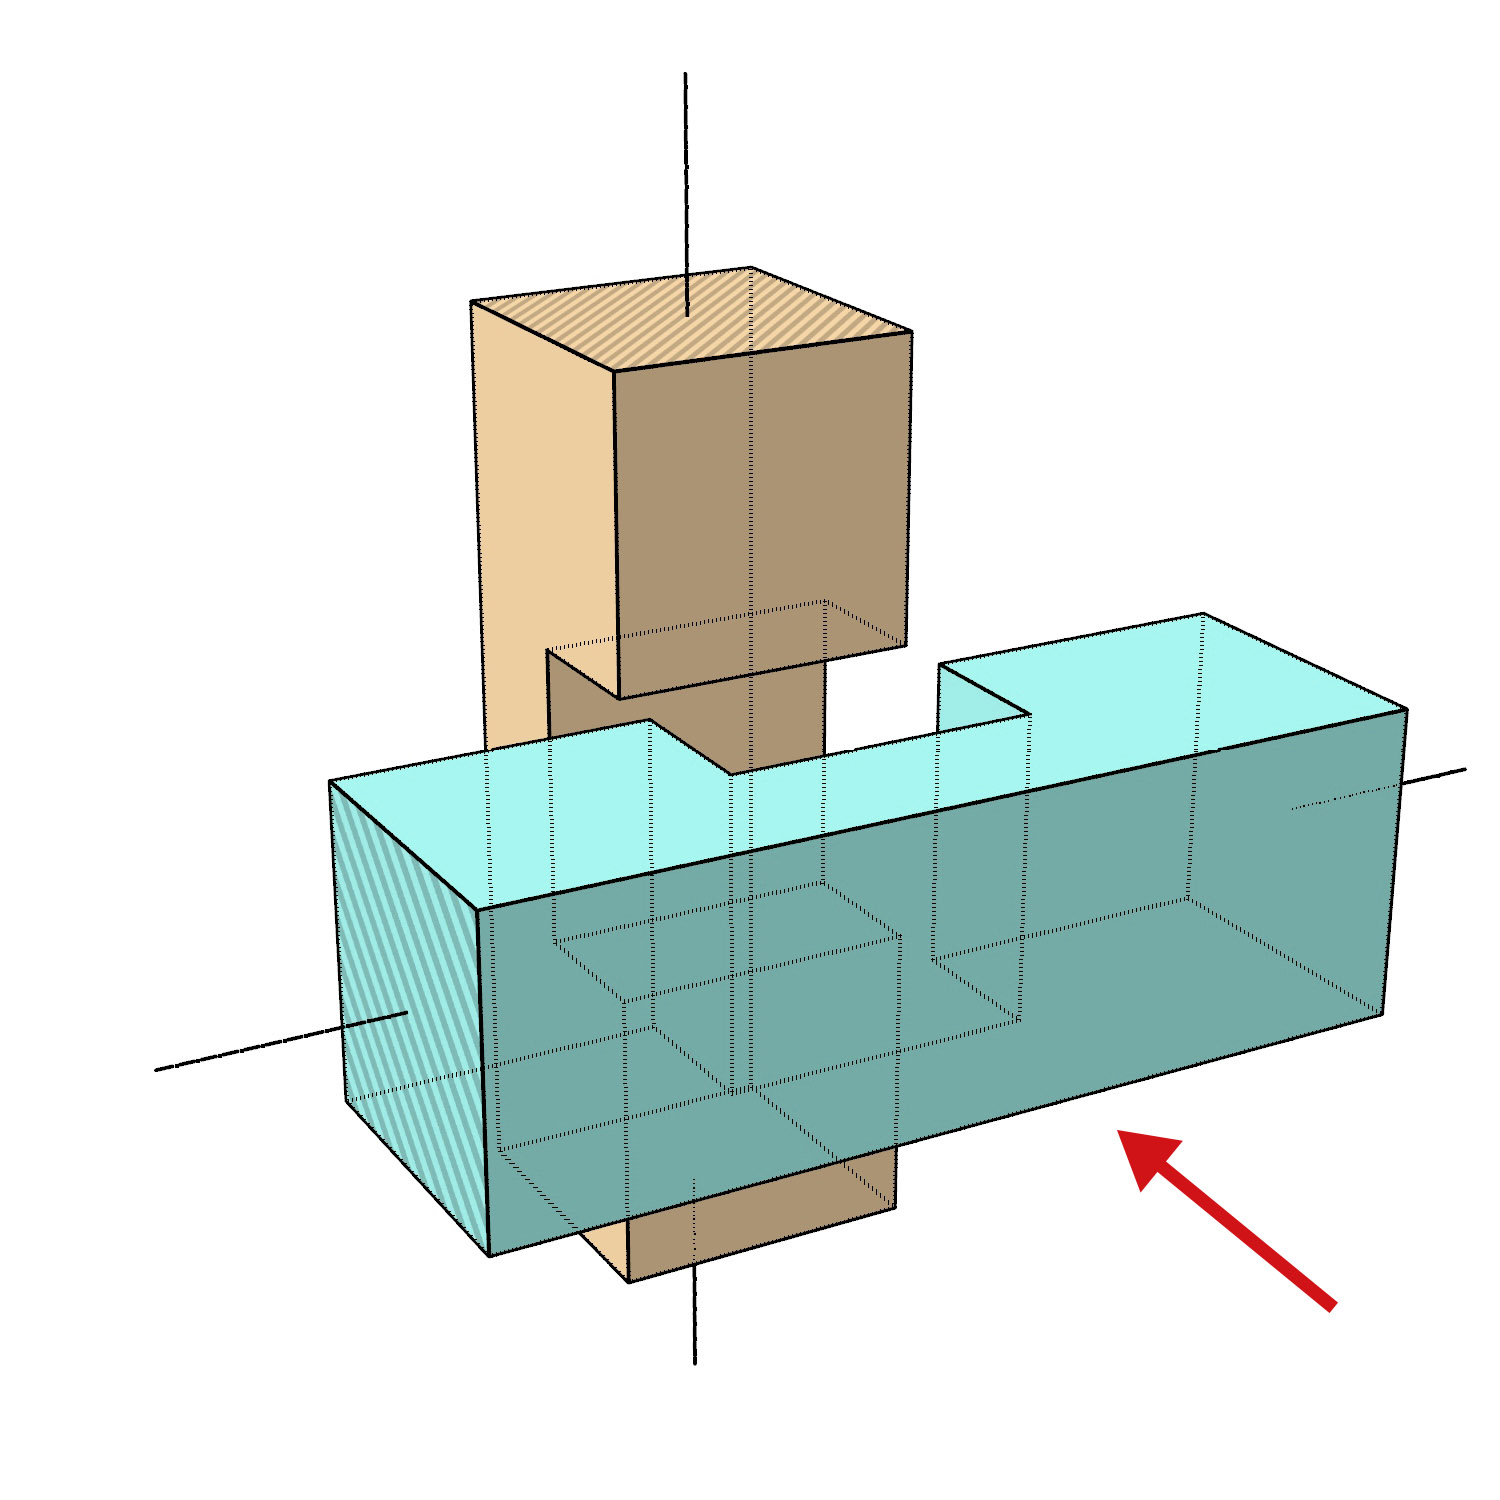
\includegraphics[width=\textwidth]{images/04-1+2/CrossLap_6_witharrows.jpg}
         \caption{Lap Joint (Cross shape)}
         \label{fig:common-joints-crosslap}
     \end{subfigure}
     \hfill
     \begin{subfigure}[b]{0.32\textwidth}
         \centering
         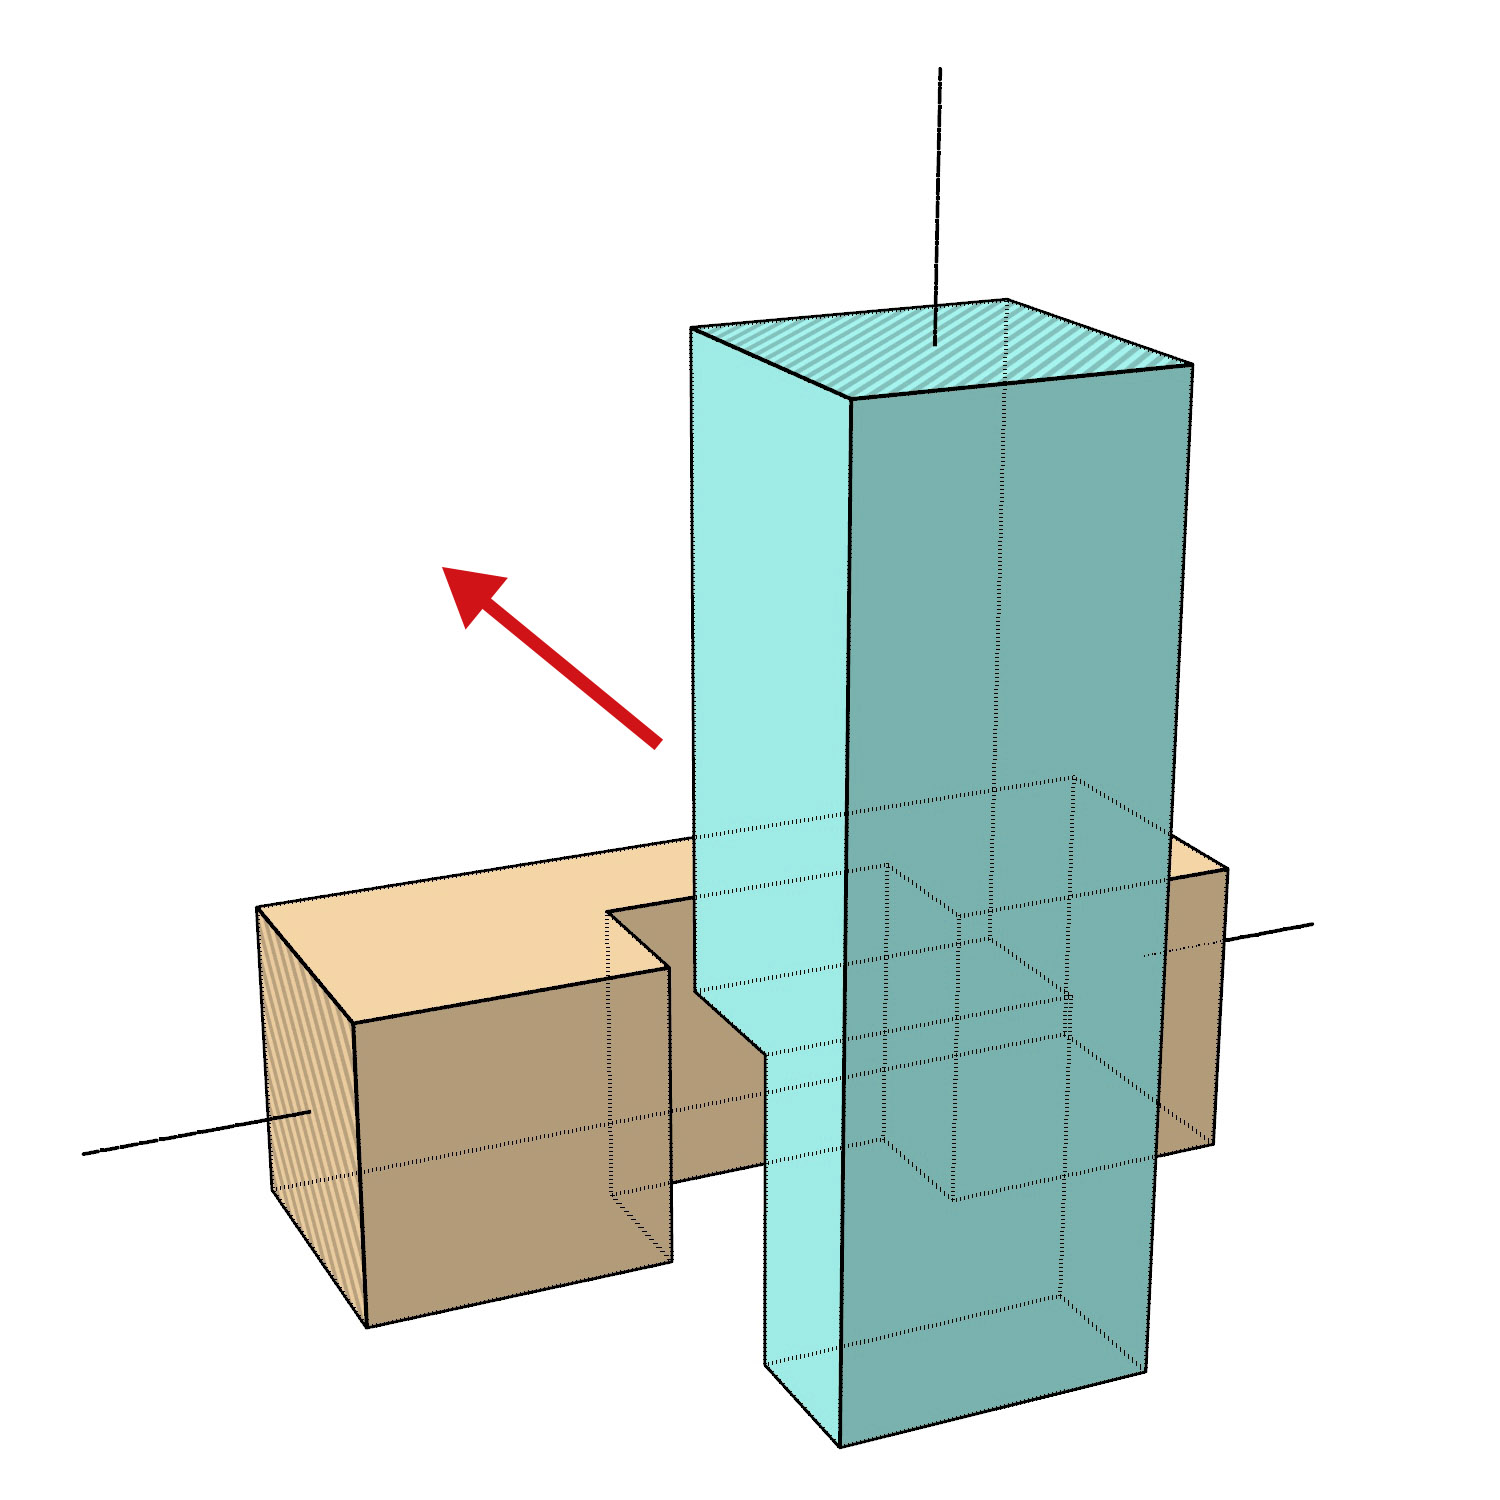
\includegraphics[width=\textwidth]{images/04-1+2/TeeLap_6_witharrows.jpg}
         \caption{Lap Joint (Tee shape)}
         \label{fig:common-joints-teelap}
     \end{subfigure}
     \hfill
     \begin{subfigure}[b]{0.32\textwidth}
         \centering
         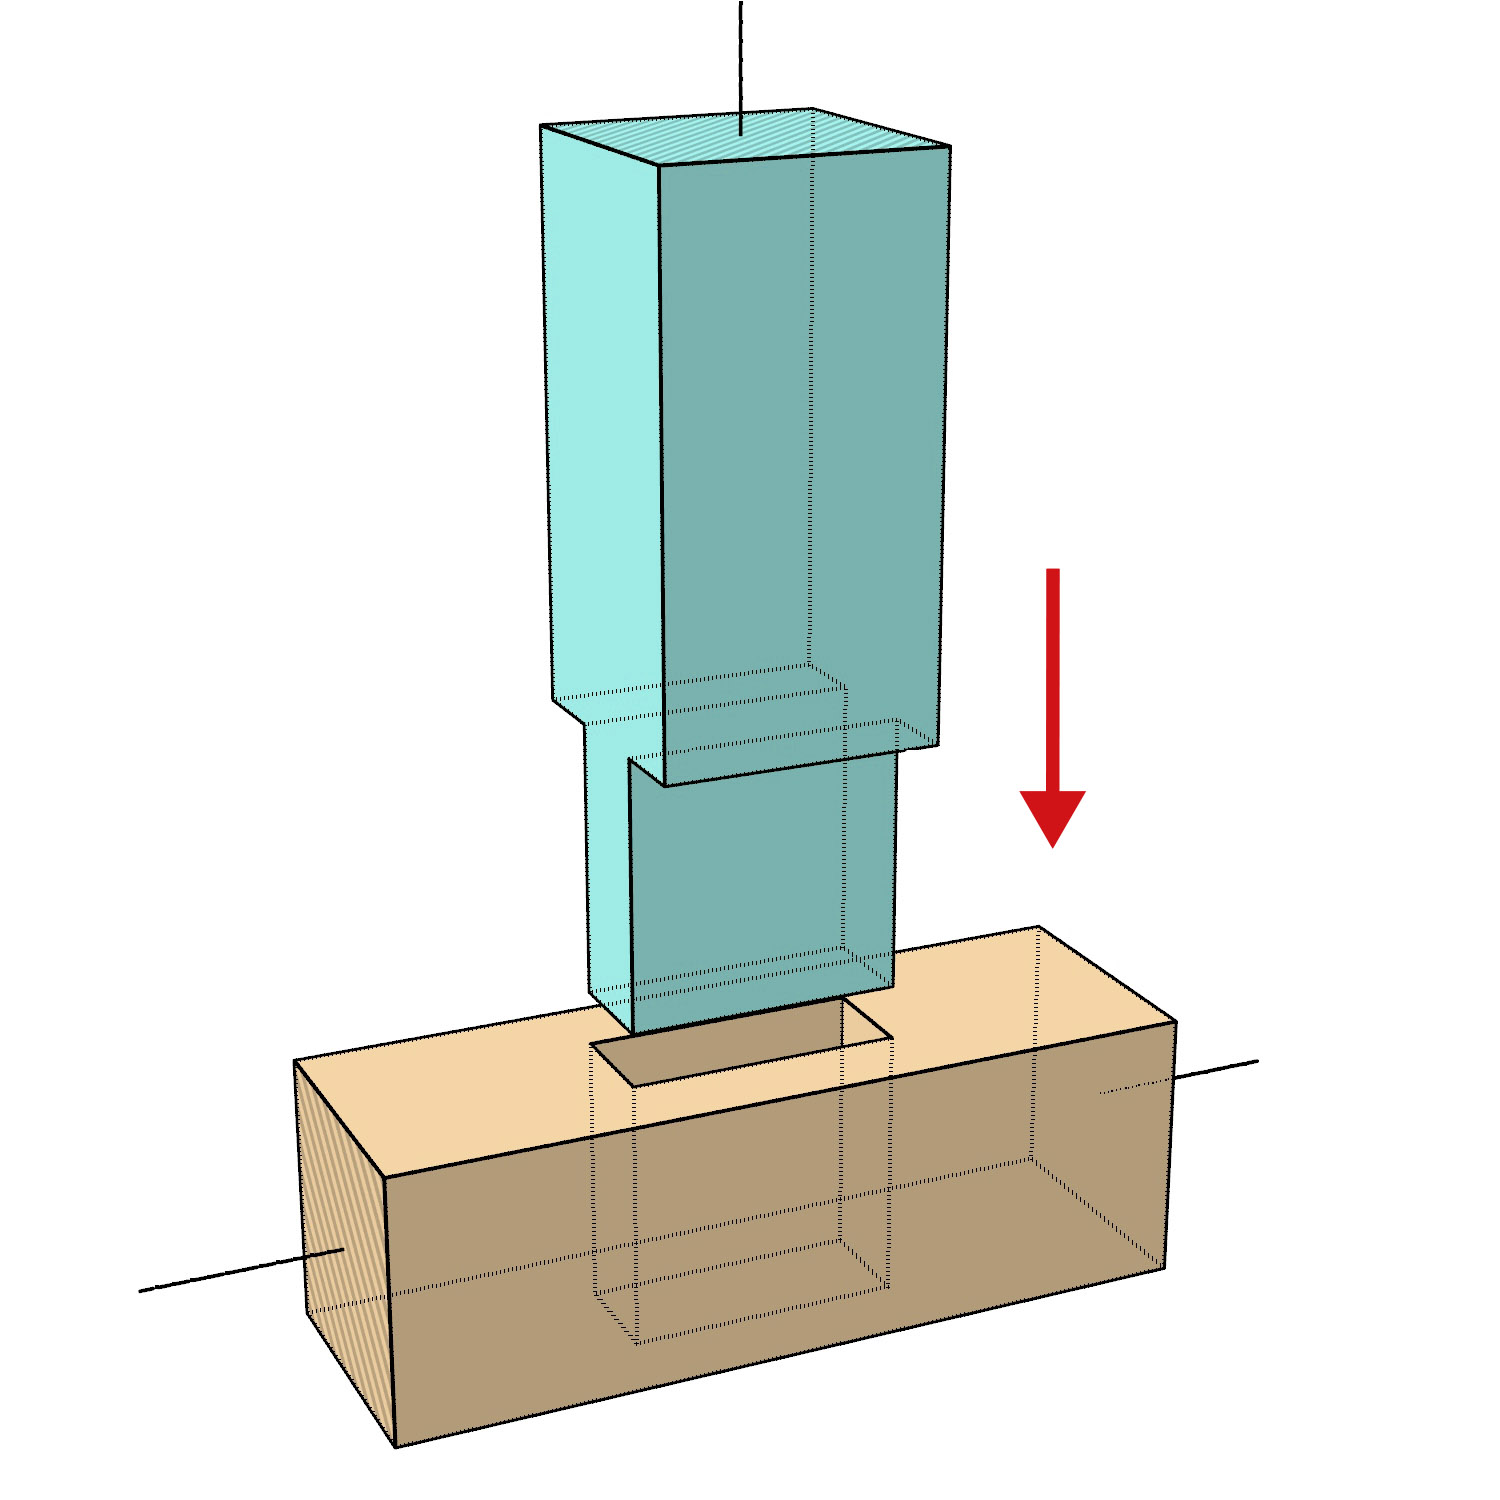
\includegraphics[width=\textwidth]{images/04-1+2/Tenon_6_witharrows.jpg}
         \caption{Mortise Tenon Joint}
         \label{fig:common-joints-mortisetenon}
     \end{subfigure}
     \caption{Diagrams of common integral timber joints used in timber frame construction}
     \label{fig:three-common-joints}
\end{figure}

\subsection{Joint Tightness}
\label{subsection:exploration-1-joint-tightness}

For the purpose of developing robotic actuators, it is necessary to quantify the force needed to assemble the lap joint. Based on my own carpentry experience and the report from a related timber joint study (Robeller et al., 2017), the assembly force for an architectural scale joint is not only related to but also highly sensitive to the fit of joint geometry. Due to the lack of relevant literature, a test was conducted to identify the force required for different joint tightness.

\subsubsection{Tightness Measurement Setup}

The samples to be tested consisted of 6 pieces of joint samples (six half sides). In order to maximise the data being collected, each joint-half was paired with others and test assembled with one another in all possible combinations, providing 15 test pairs.

The samples are made with construction grade spruce with 80mm x 80mm cross section\footnote{Note that the sample size is 80mm x 80mm, but the timber intended for this thesis is 100mm x 100mm. However, the result is good enough for the purpose of specifying the clamping force.} with a construction grade plane finish.
The shoulders of each joint were cut manually with a Japanese pull saw. The cheek width (C) and notch width (N) are measured after the joint is cut (see Figure \ref{fig:lap-joint-assembly-rubbing-before}), multiple points were measured with a caliper with 0.01mm resolution and their mean value is recorded.

\begin{figure}
    \centering
    \begin{subfigure}[b]{0.49\textwidth}
        \centering
        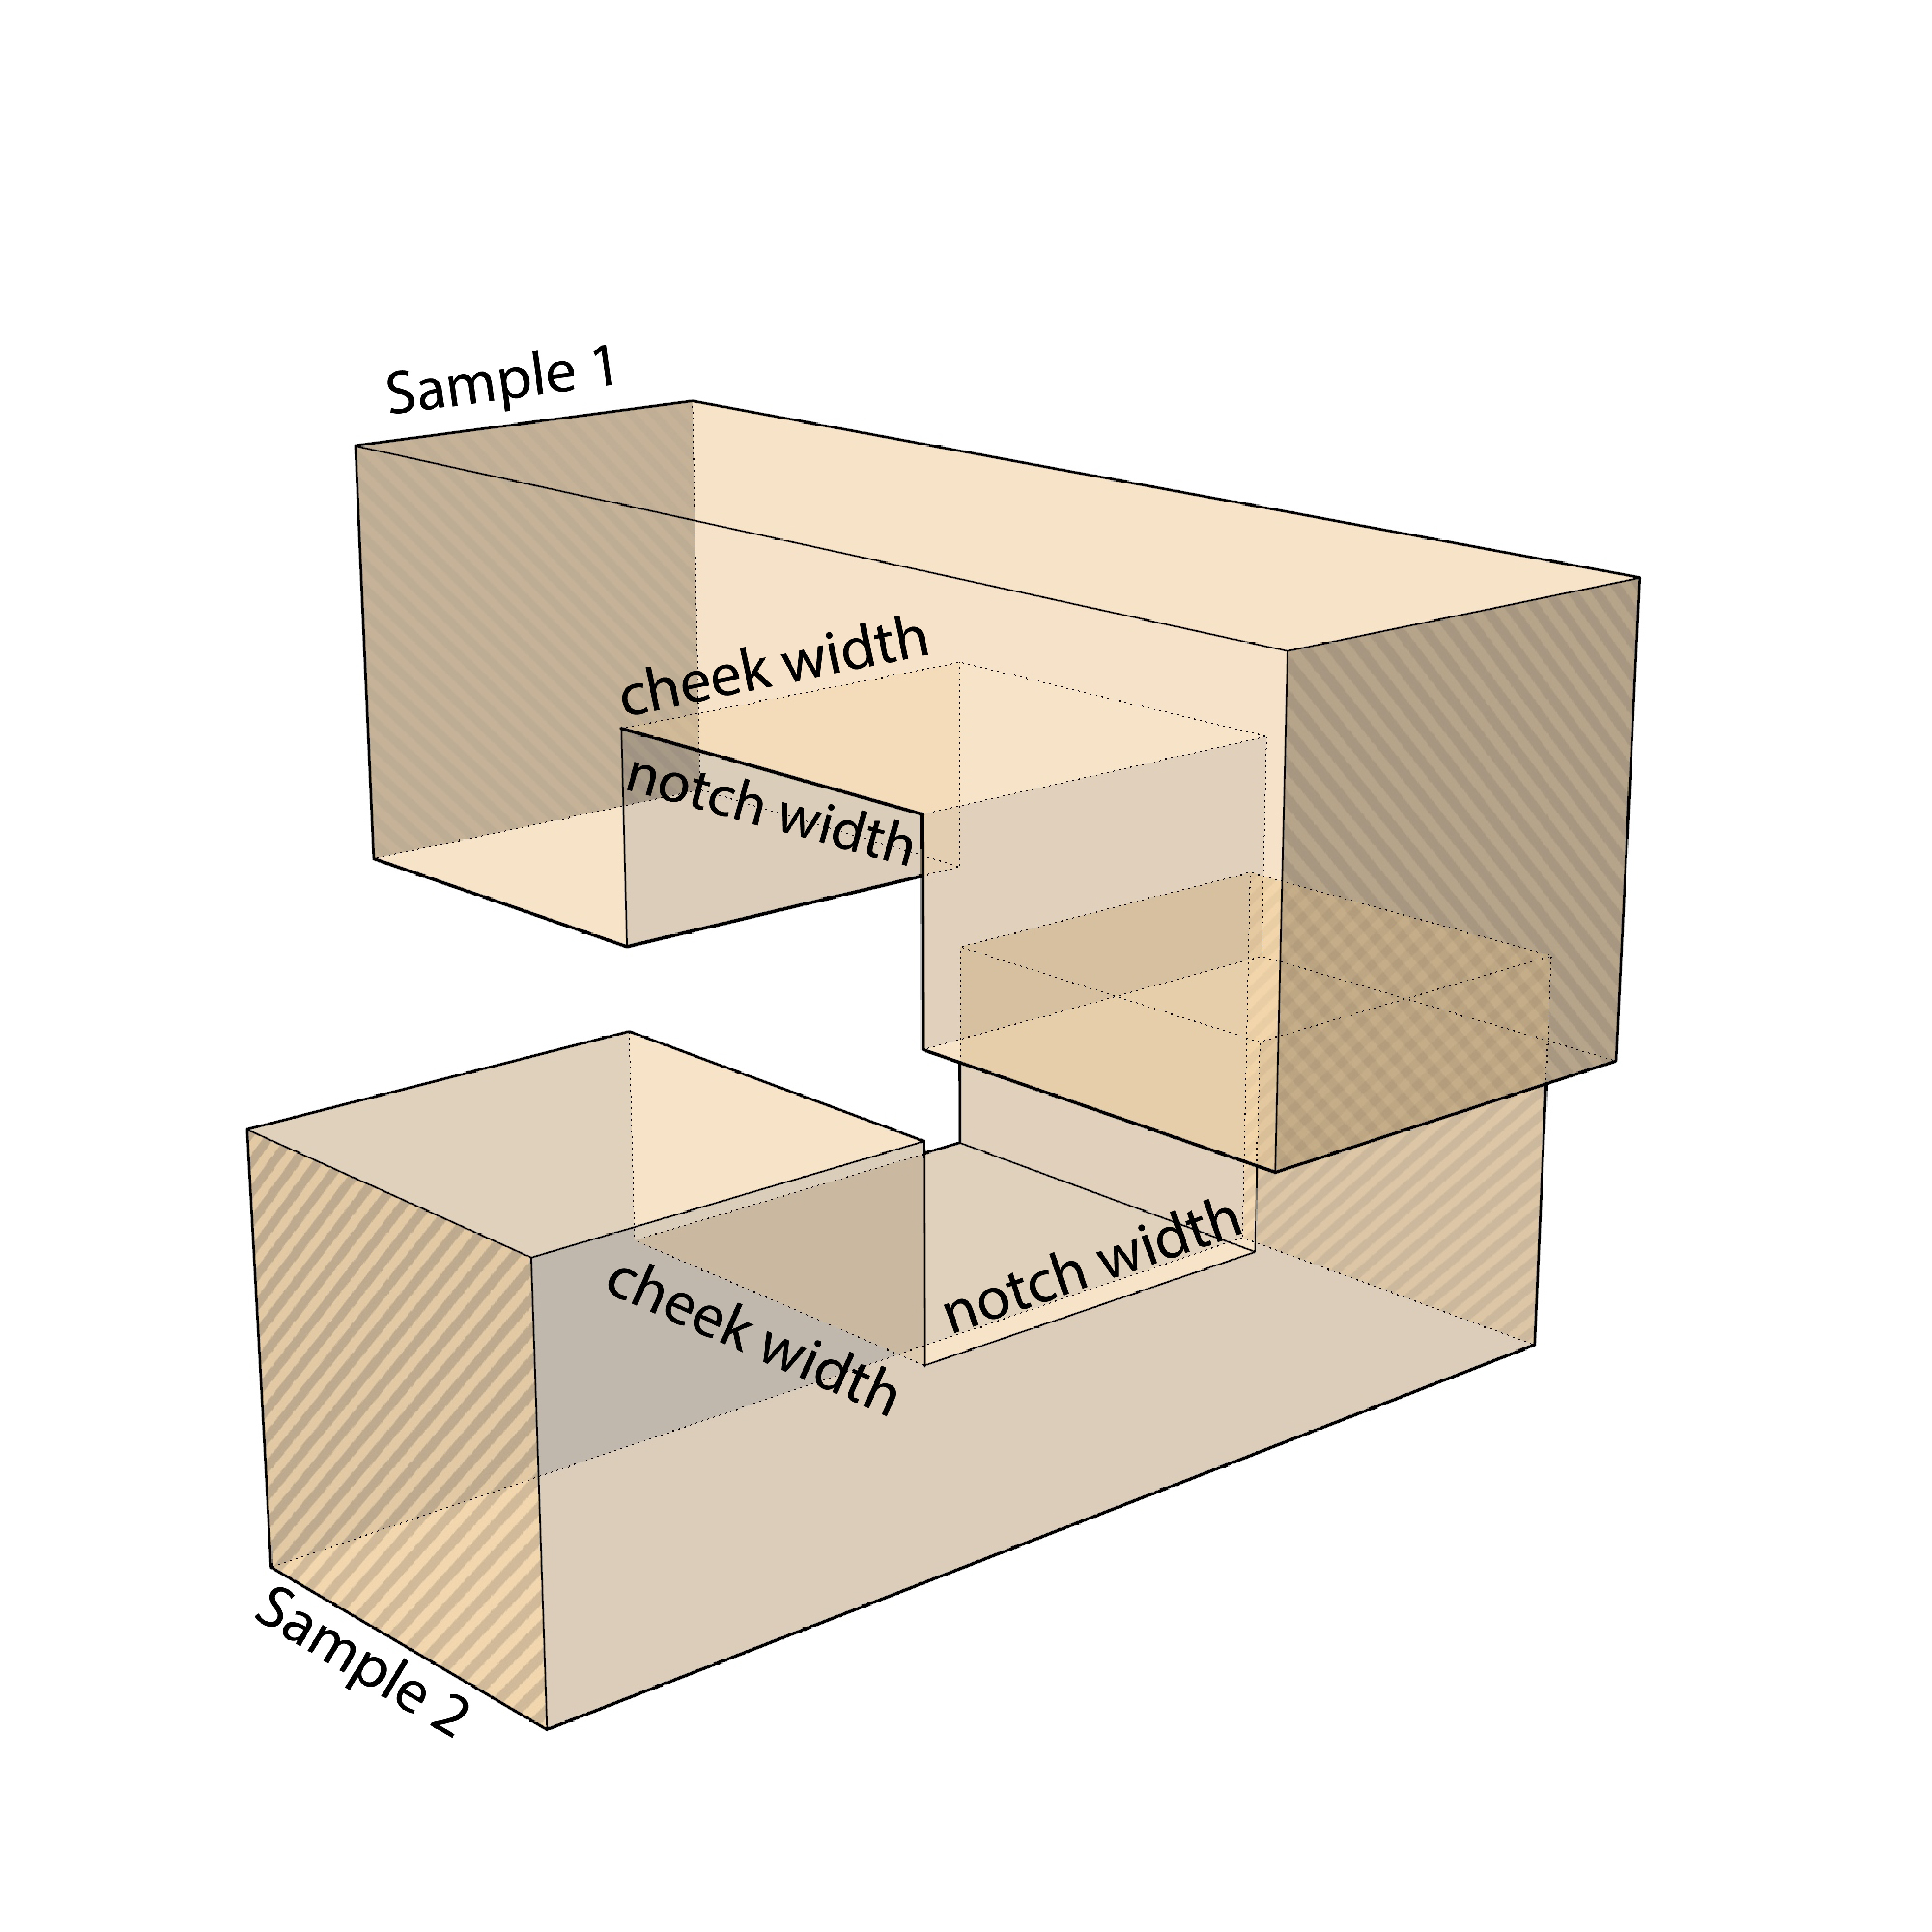
\includegraphics[width=\textwidth]{images/04-1+2/tightness-measurement.jpg}
        \caption{Before Assembly}
        \label{fig:lap-joint-assembly-rubbing-before}
    \end{subfigure}
    \hfill
    \begin{subfigure}[b]{0.49\textwidth}
        \centering
        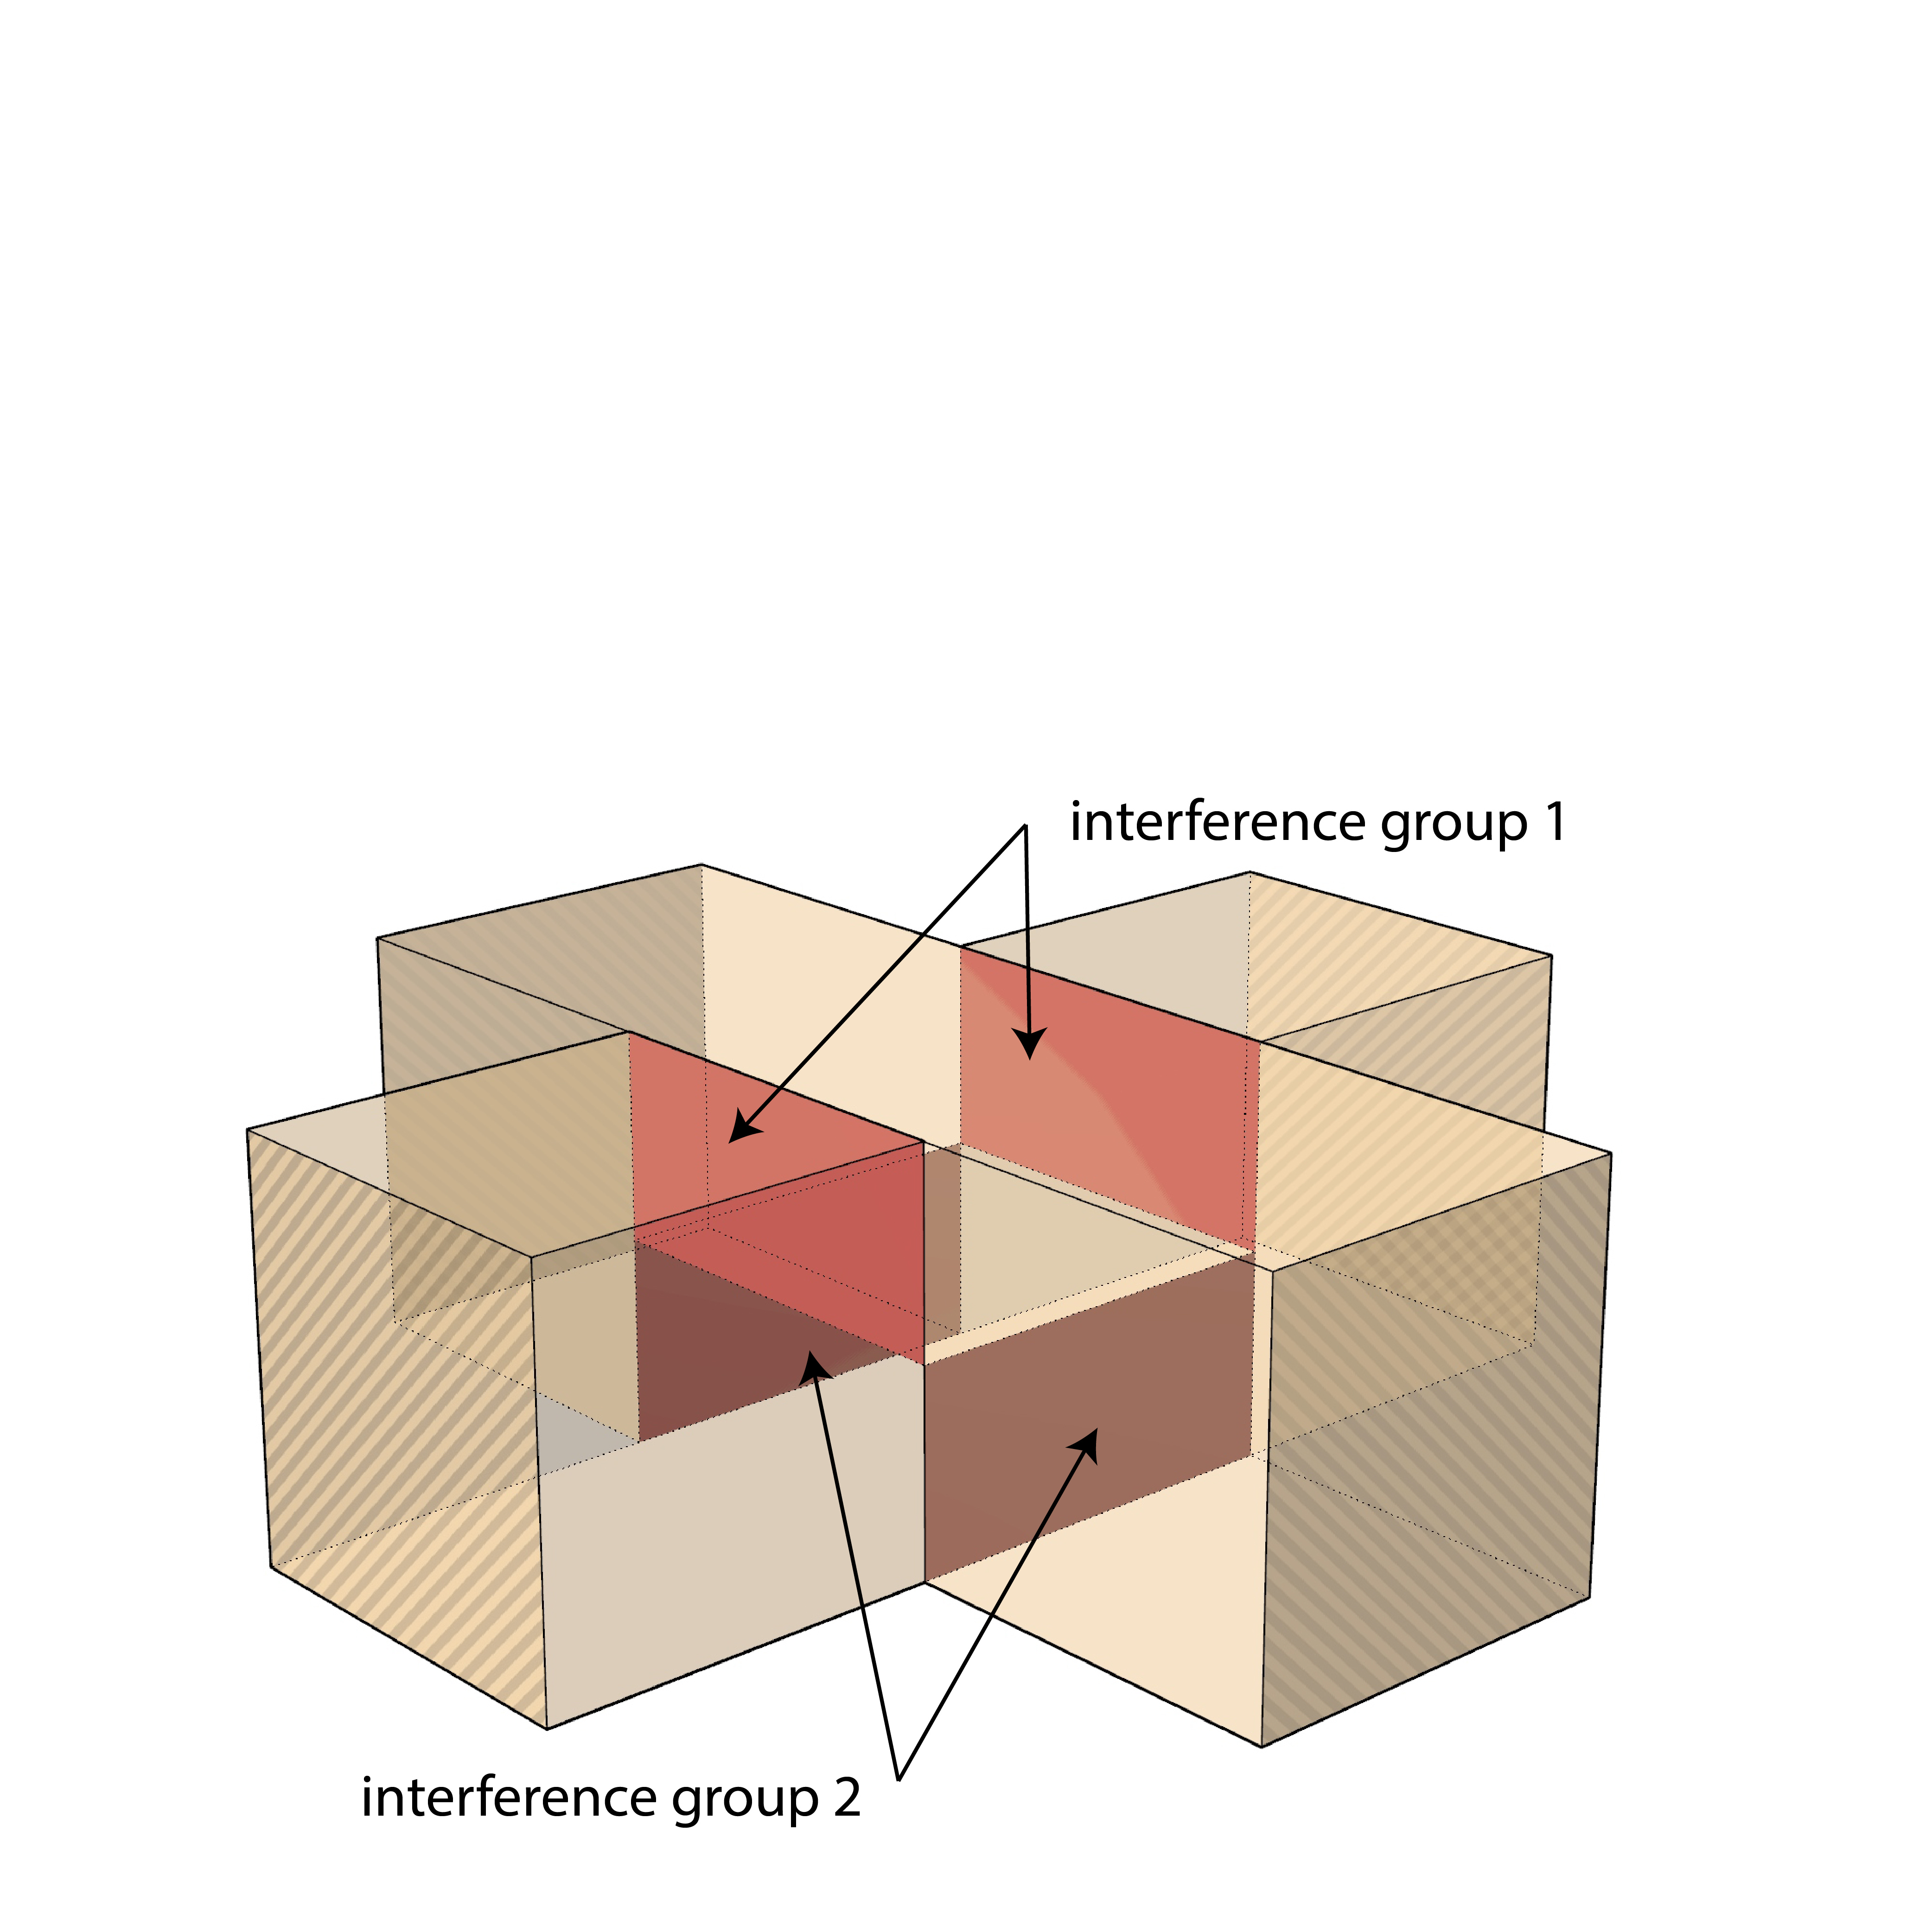
\includegraphics[width=\textwidth]{images/04-1+2/tightness-rubsurface.jpg}
        \caption{After Assembly}
        \label{fig:lap-joint-assembly-rubbing-after}
    \end{subfigure}
    \caption{Diagram showing surfaces (red) that are in rubbing contact during assembly}
    \label{fig:lap-joint-assembly-rubbing}
\end{figure}


Figure \ref{fig:lap-joint-assembly-rubbing-after} shows four surfaces that were expected to be in tight rubbing contact, contributing to assembly resistance. These surfaces come in two interference groups (IG). Interference for each group can be computed by the following formula. Note that the value is positive when there is interference. The case where the joint is loose, it is assumed to have 0 interference. 

Interference of IG 1 = $max( C (Sample 1) - N (Sample 2), 0)$\\
Interference of IG 2 = $max( C (Sample 2) - N (Sample 1), 0)$

The mean interference between the two groups is used as an indication of the tightness of a joint. The larger the interference, the tight the joint. Figure \ref{fig:interference-amount} shows the computed mean interference for each Interference Group. The force-measurement setup consists of a manually actuated carpentry clamp compressing on a digital load cell which compresses the lap joint (see Figure \ref{fig:interference-measurement-setup}). The force during the assembly was logged and filtered and the maximum value was taken to represent the assembly force of the sample. Care was taken to not completely close the joint to ensure that the measured force was representing the kinematic part of the closure. If the cheeks of the lap joint were in contact, the measurement would be related to the stall force.

\begin{figure}
    \centering
    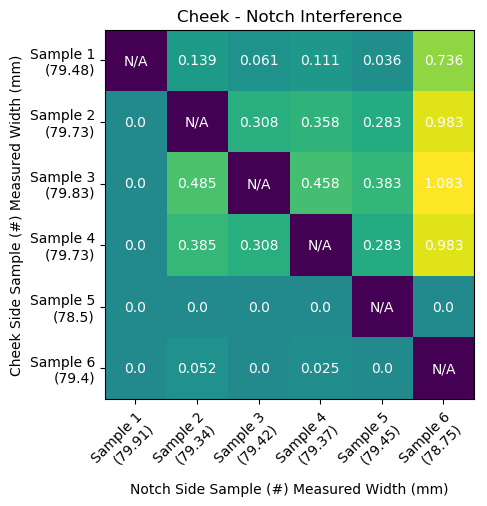
\includegraphics[width=0.6\textwidth]{images/04-1+2/tightness-pairwise-size.png}
    \caption{Amount of interference (mm) between between the sample pair}
    \label{fig:interference-amount}
\end{figure}

\begin{figure}
    \centering
    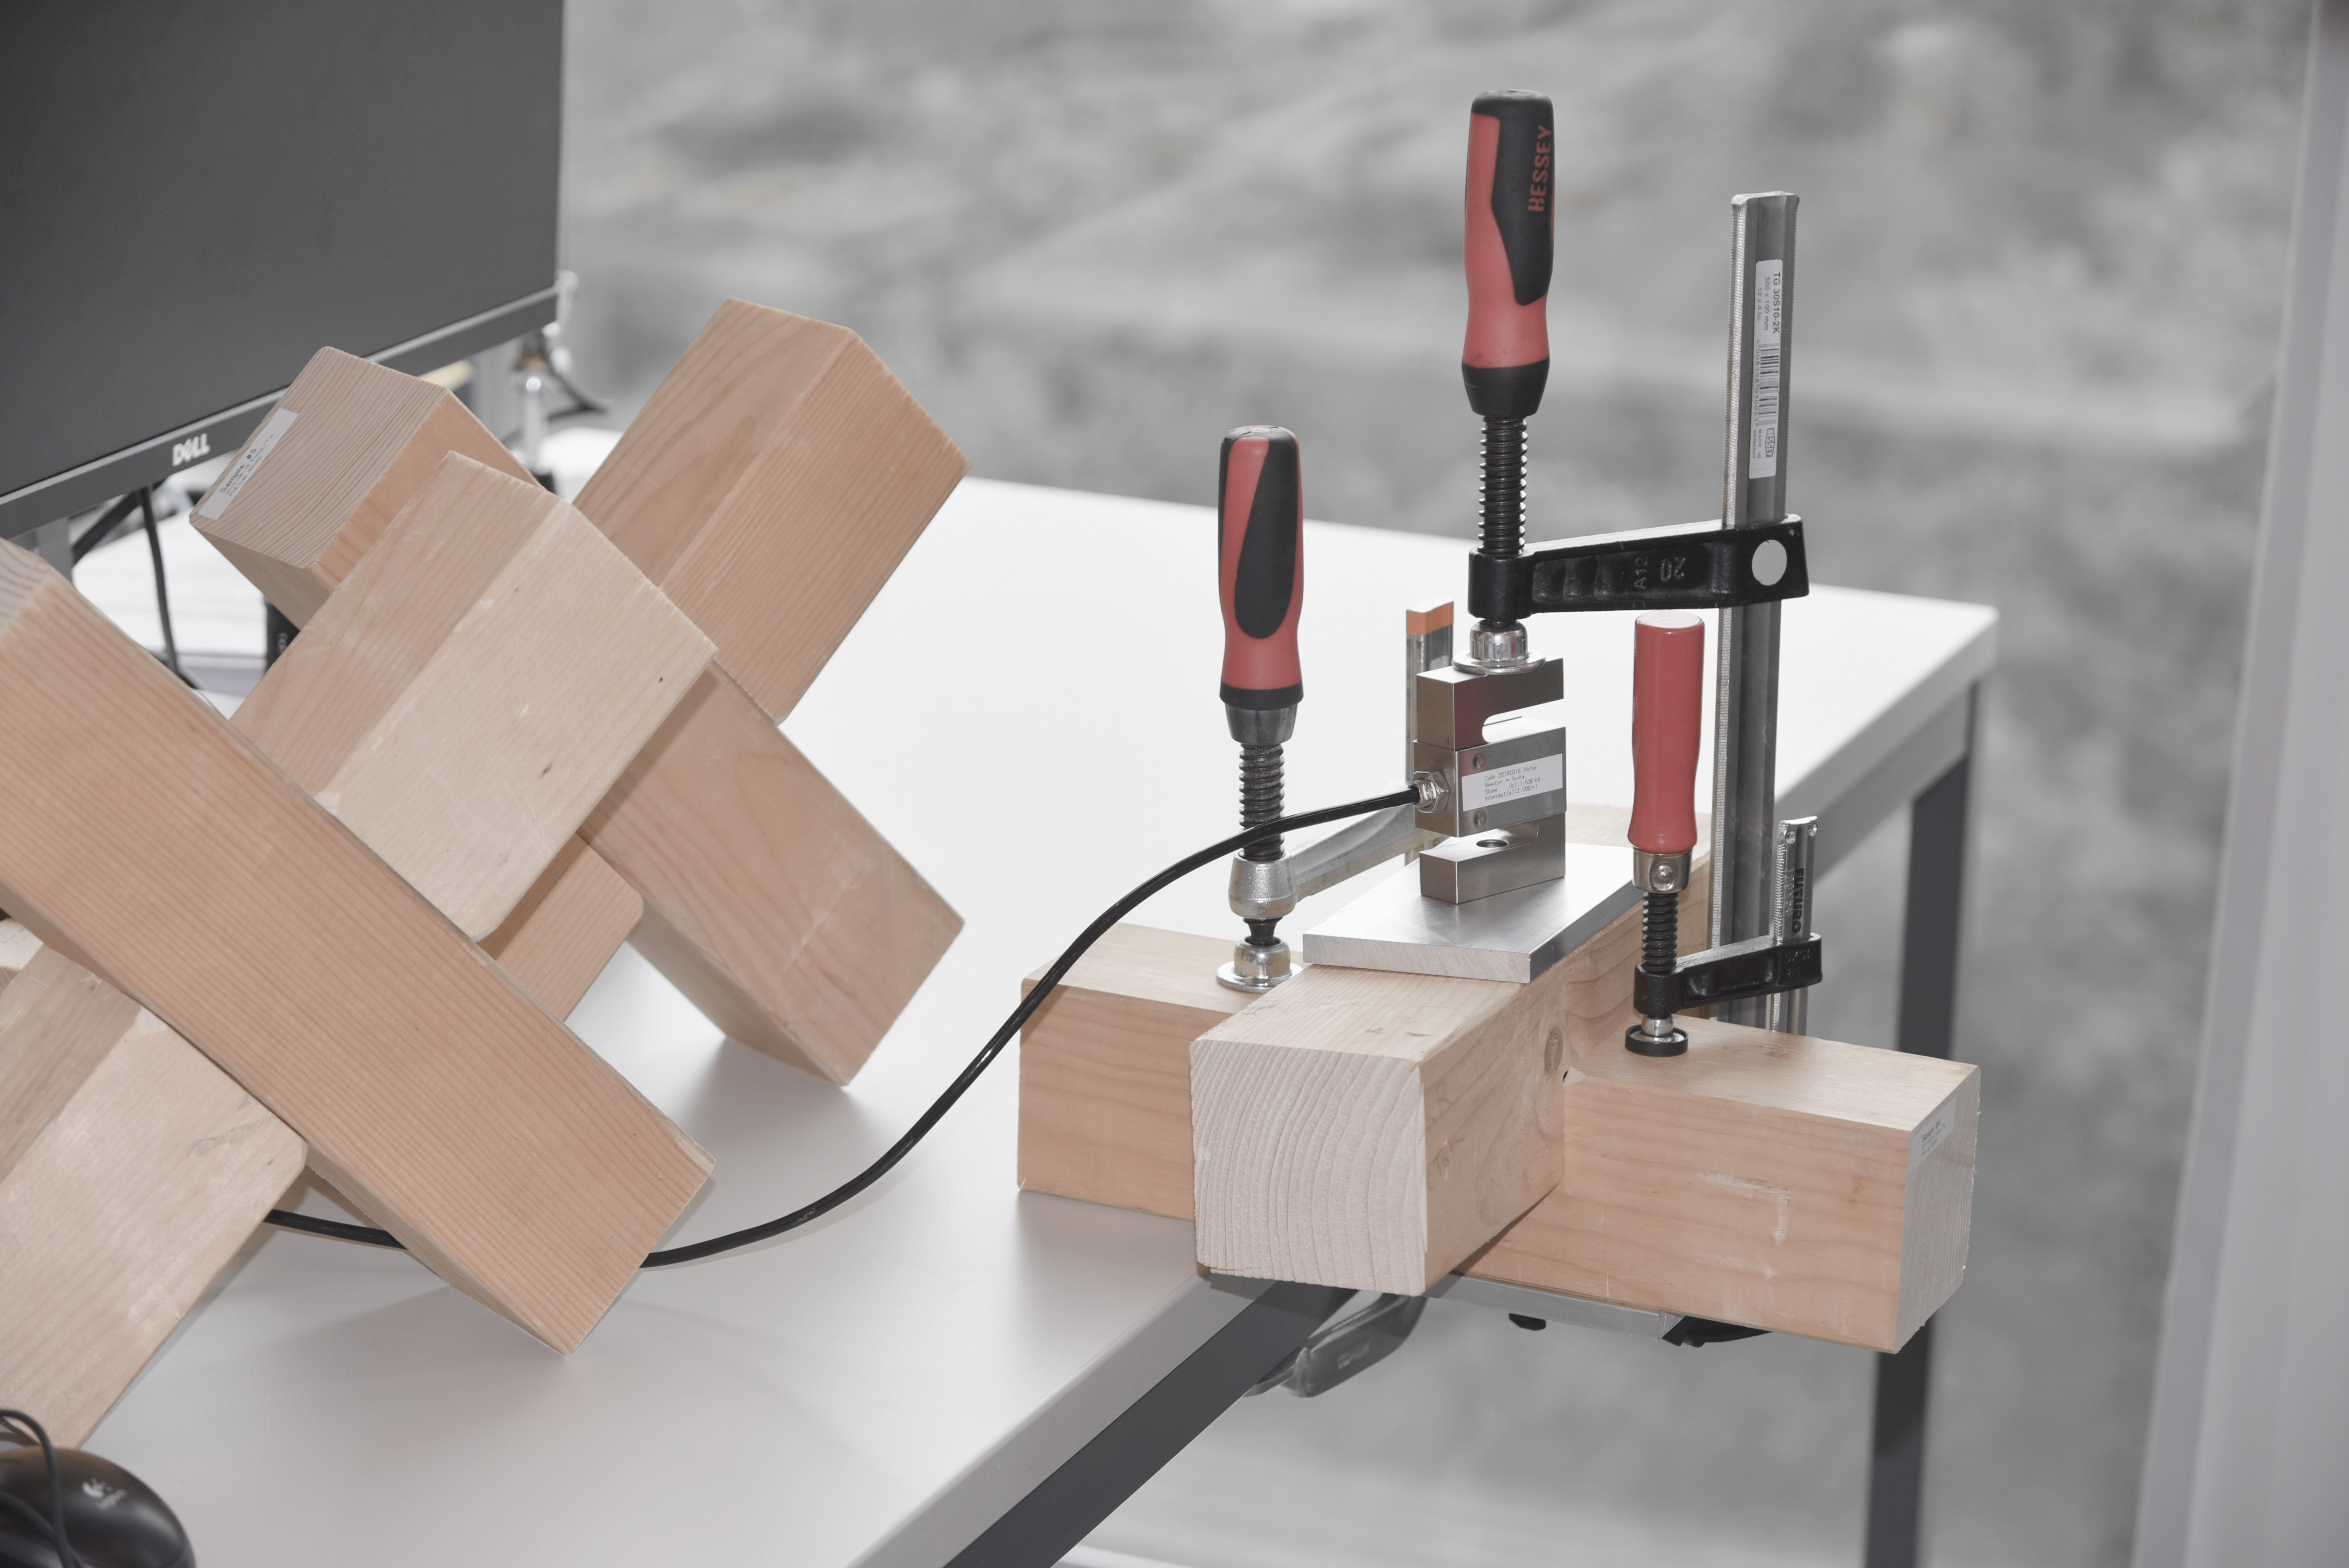
\includegraphics[width=0.99\textwidth]{images/04-1+2/setup.jpg}
    \caption{Setup for measuring closure force of lap joint samples}
    \label{fig:interference-measurement-setup}
\end{figure}

\subsubsection{Results and Conclusion about Joint Tightness}

Figure \ref{fig:tightness-measurement-pairwise} shows the pairwise force measurement result. Sample 1-4 was not measured because it had no friction at all. Sample 4-6 cannot be measured because it was too tight to begin any assembly motion. Figure \ref{fig:tightness-measurement-plot} shows the relationship between the mean interference (representing tightness) and the assembly force needed. 

\begin{figure}[H]
    \centering
    \begin{subfigure}[b]{0.40\textwidth}
        \centering
        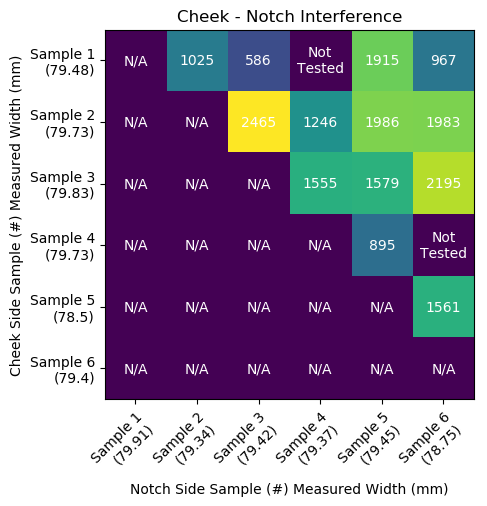
\includegraphics[width=\textwidth]{images/04-1+2/tightness-pairwise-result.png}
        \caption{Measurement result between pairs of samples}
        \label{fig:tightness-measurement-pairwise}
    \end{subfigure}
    \hfill
    \begin{subfigure}[b]{0.58\textwidth}
        \centering
        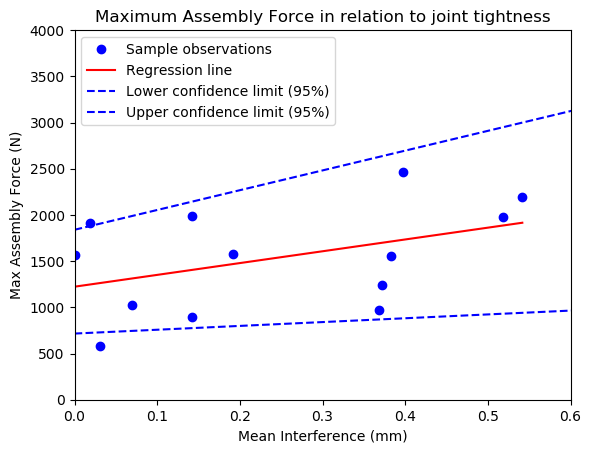
\includegraphics[width=\textwidth]{images/04-1+2/tightness-result-plot.png}
        \caption{Assembly force plot against interference between sample pairs}
        \label{fig:tightness-measurement-plot}
    \end{subfigure}
    \caption{Tightness measurement result}
    \label{fig:tightness-measurement-result}
\end{figure}

While it is not possible to conclude the correlation between the two quantities based on a few data samples, the test has shown a reasonable upper force limit for specifying the linear actuator. The forces measured are in the same order of magnitude as the number reported by a previous study (Robeller et al., 2017). For the purpose of designing the clamp actuator, the required clamping force was specified at 3000N. 

\section{Development}
\label{section:exploration-1-development}

\subsection{Lap Clamp CL1}
\label{subsection:exploration-1-lap-clamp-cl1-proof-of-concept}

The Lap Clamp CL1 was designed as a proof of concept clamp to demonstrate the robotic clamping action. The goal is to assemble a single orthogonal half-lap joint on a 100mm timber profile. 
In addition, it contains a spring-loaded parallel gripper mechanism to allow it to hang onto the structure. Figure \ref{fig:cl1-sketch} shows an early sketch of the clamp design, showing a U-shape configuration that surrounds a beam.

\begin{figure}
    \centering
    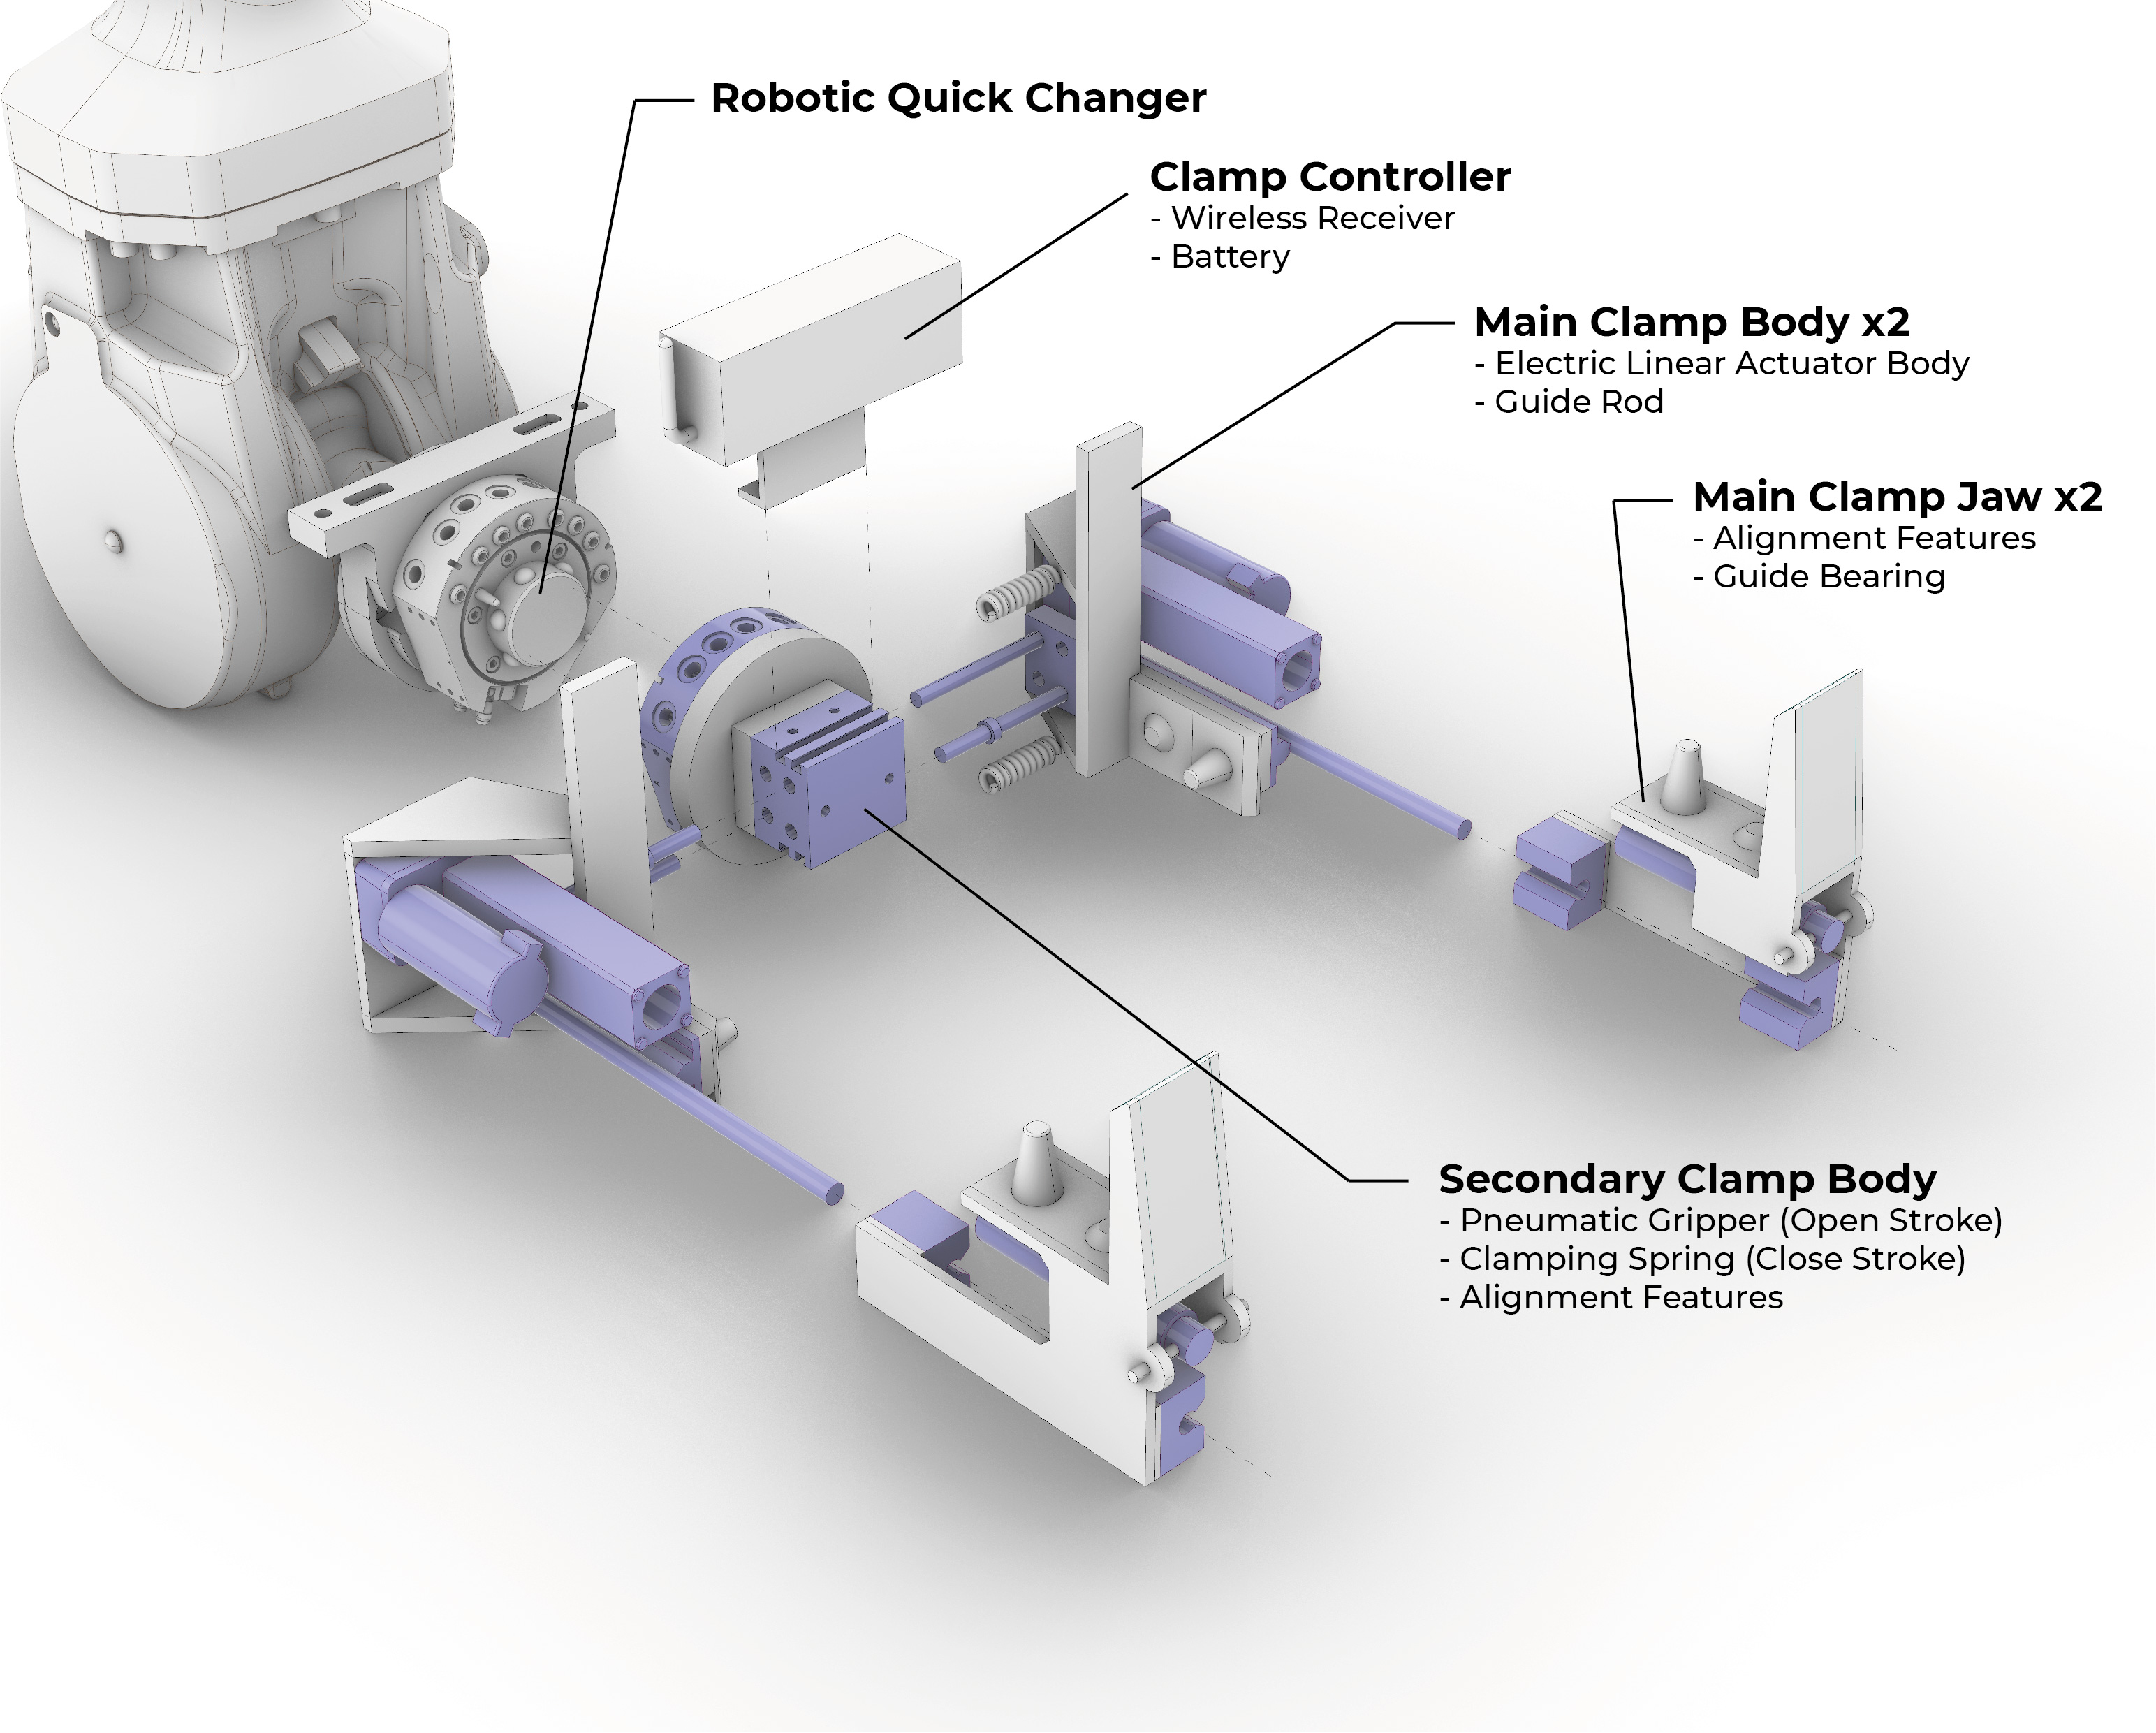
\includegraphics[width=0.99\textwidth]{images/04-3/cl1-exploded-diagram.jpg}
    \caption{Sketch drawing of the CL1 clamp design showing the U-shape configuration}
    \label{fig:cl1-sketch}
\end{figure}

\subsubsection{Linear Actuator and Jaw Design}
\label{subsubsection:exploration-1-linear-actuator-and-jaw-design}

The robotic clamp jaw is designed around a linear actuator typically used for movable furniture (see Figure \ref{fig:linear-actuator-cl1}), it has a compact design and is rated for 2000N of force at 5mm/s. Despite the force being lower than the 3000N requirement established in \noseeref{subsection:exploration-1-joint-tightness}, using two jaws combined would likely be sufficient to overcome the tightest joint. The motor contains a 2-channel hall effect encoder fixed to the motor shaft, this is needed for closed loop position control \seeref{subsubsection:exploration-1-bang-bang-motion-control}. 

\begin{figure}[hb!]
    \centering
    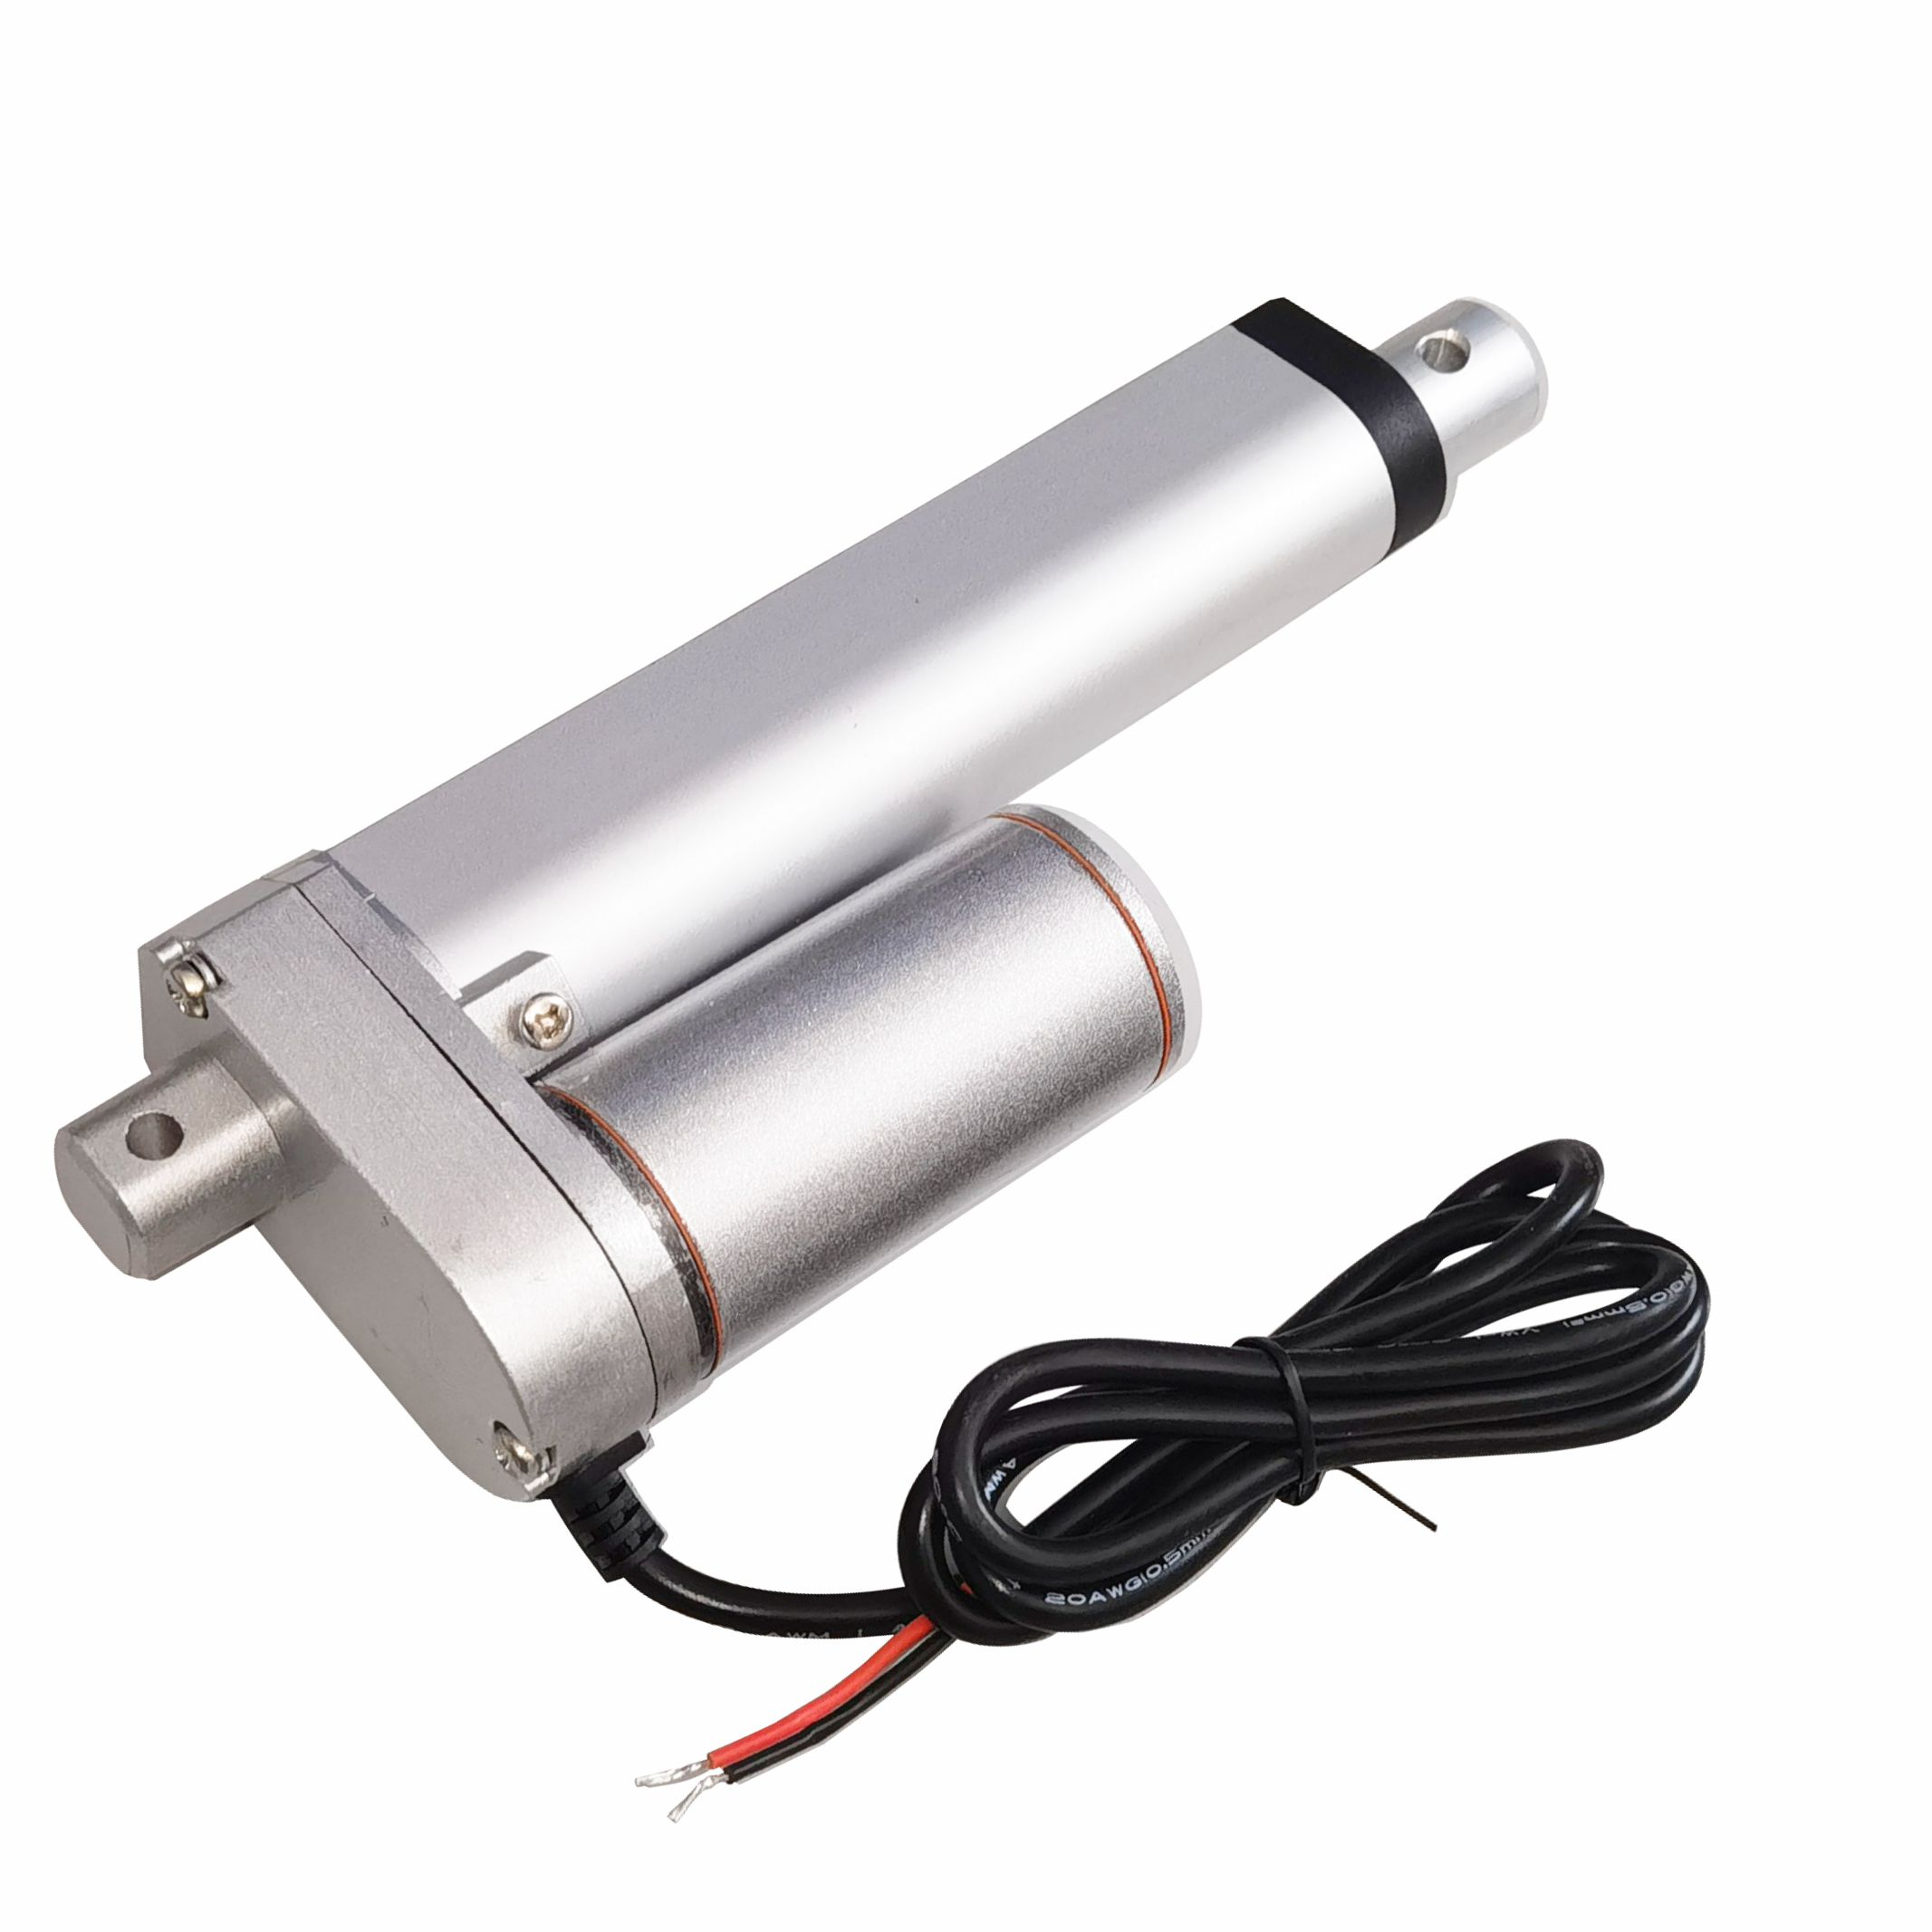
\includegraphics[width=0.99\textwidth]{images/04-3/cl1-linearactuator.jpg}
    \caption{Linear actuator used in the CL1 clamp}
    \label{fig:linear-actuator-cl1} 
\end{figure}

The clamp jaw is made from aluminium plates bolted together. It has two open-type bronze linear bushing paired with a 12mm round shaft to act as linear motion guide. The bronze bearing was chosen over ball-type linear bearings to maximise load capacity. The front side of the actuator is mounted with an in-line load cell for collecting force data for analysis. Figure \ref{fig:cl1-clamp-jaw} shows the detached clamp jaw from the guide shaft and linear actuator. 

\begin{figure}
    \centering
    \begin{subfigure}[b]{0.49\textwidth}
        \centering
        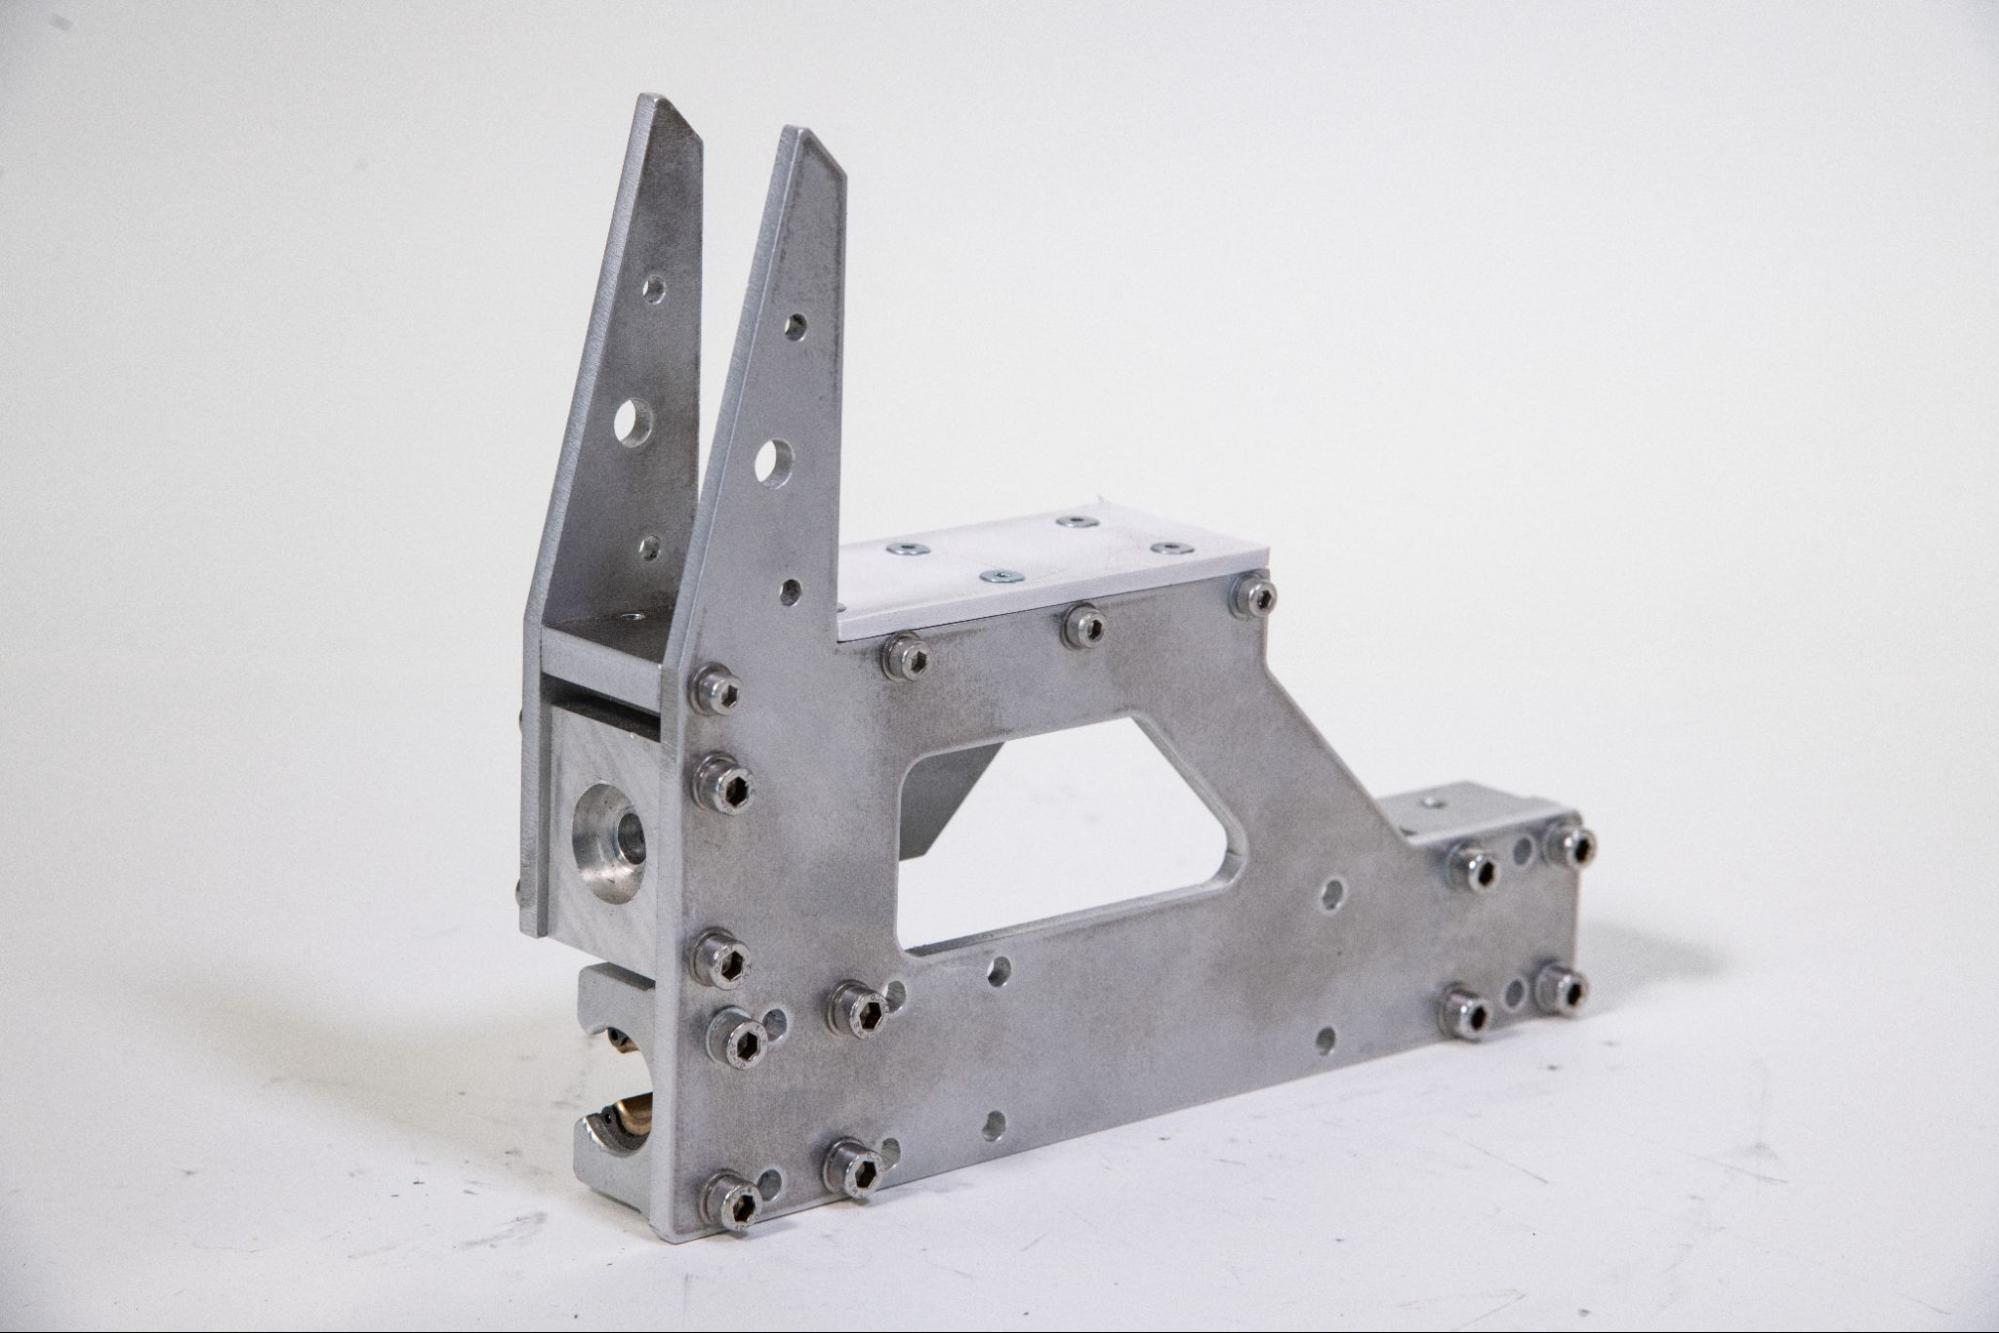
\includegraphics[width=\textwidth]{images/04-3/cl1-jaw-left.jpg}
        % \caption{SubFigureCaption}
        %\label{fig:uniquesubfigurelabel}
    \end{subfigure}
    \hfill
    \begin{subfigure}[b]{0.49\textwidth}
        \centering
        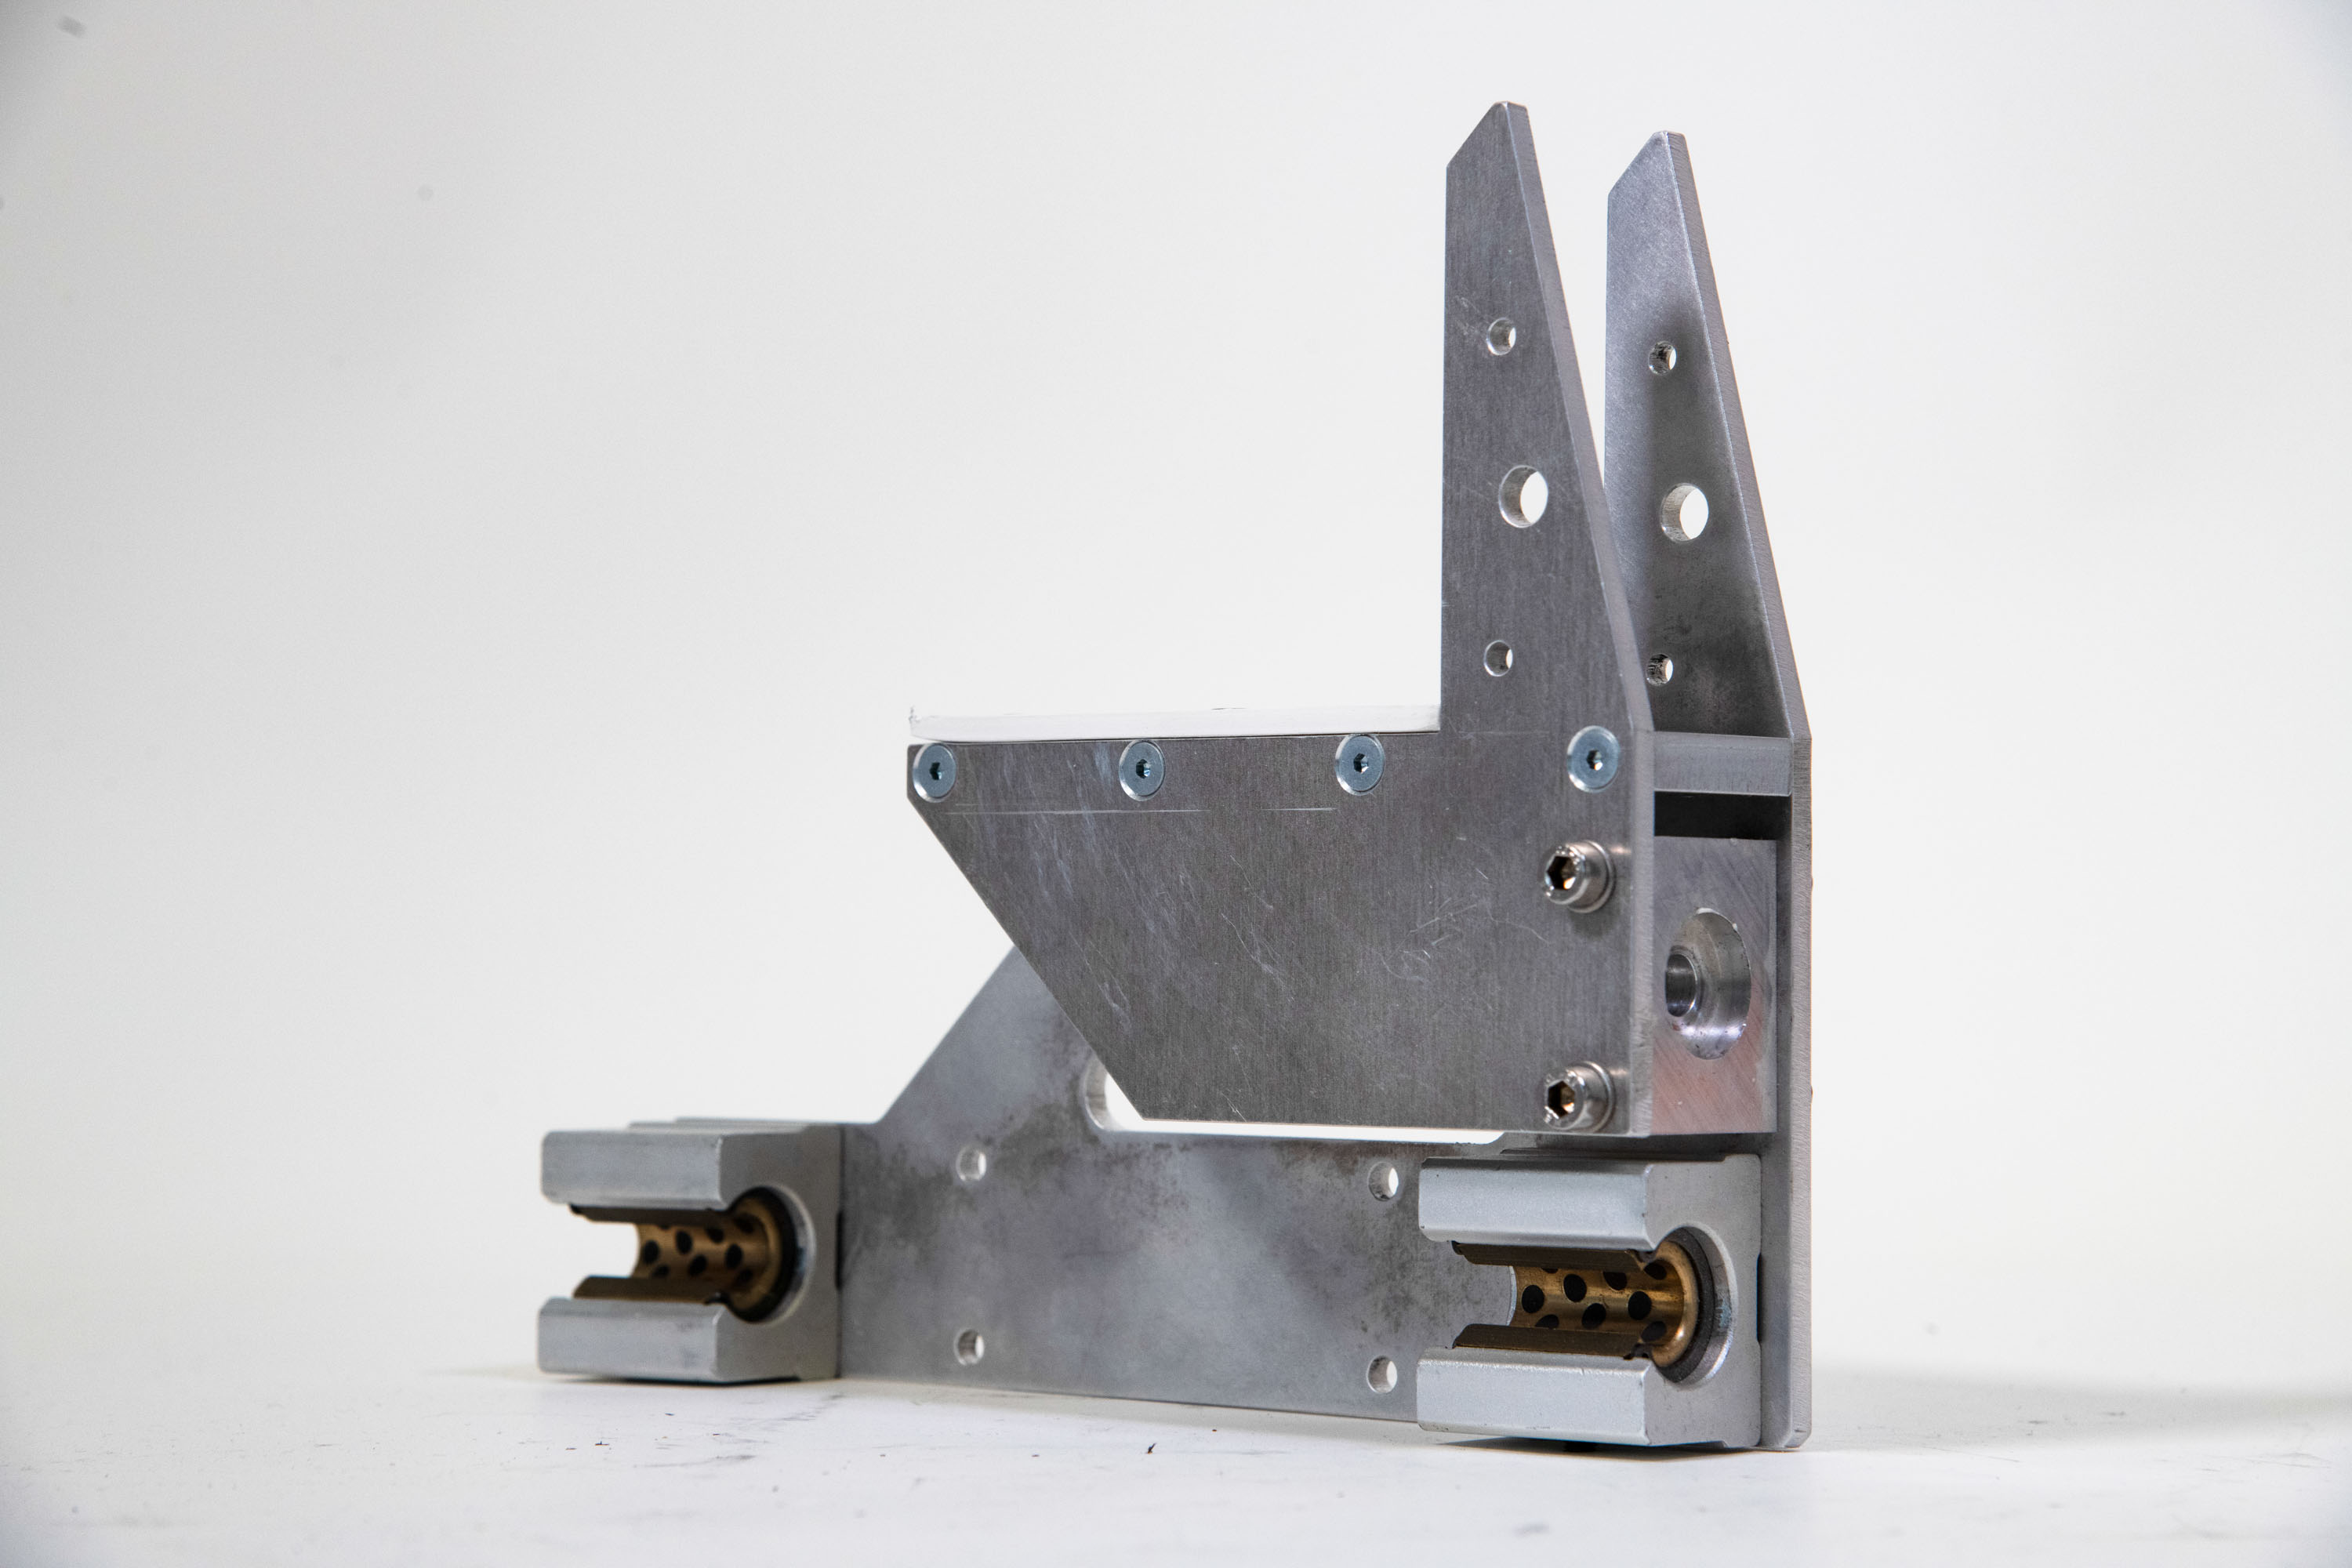
\includegraphics[width=\textwidth]{images/04-3/jaw-right.jpg}
        % \caption{SubFigureCaption}
        %\label{fig:uniquesubfigurelabel}
    \end{subfigure}
    \caption[Photo of the detached clamp jaw from the guide shaft and linear actuator]
    {Photo of the detached clamp jaw from the guide shaft and linear actuator, two bronze bushing is visible on the right image}
    \label{fig:cl1-clamp-jaw}
\end{figure}

\subsubsection{Gripper for Hanging Clamp}
\label{subsubsection:exploration-1-gripper-for-hanging-clamp}

The clamp consists of two symmetrically designed jaws and actuators. They are connected to a common body through a pneumatic parallel gripper. This parallel gripper allows a linear closing motion for the two sides of the clamp jaw to close onto a beam.
The contact surface between the clamp jaw and the timber has a 3D-printed plastic plate with pin features to allow better grappling and secure hanging. A tension spring is used to keep the gripper closed and it can only be opened when the device is docked to the robotic arm and compressed air is provided through the docking adapter. This is intended to be a safety feature, such that the clamp cannot fall on its own due to control error.

Figure \ref{fig:hanging-gripper-test} shows the parallel gripper mechanism and alignment features (the black area) being tested separately from the rest of the clamp. The position of the pins and their geometry were iterated for a few times before settling on this design. The challenge is that the external geometry of the timber beams have a large production tolerance, the location of the drilled holes can also be inaccurate. Therefore, the geometry of the L-shaped pad and the pins must accommodate this error such that the gripper can close completely and maintain a rigid hanging hold afterwards.

\begin{figure}[h!]
    \centering
    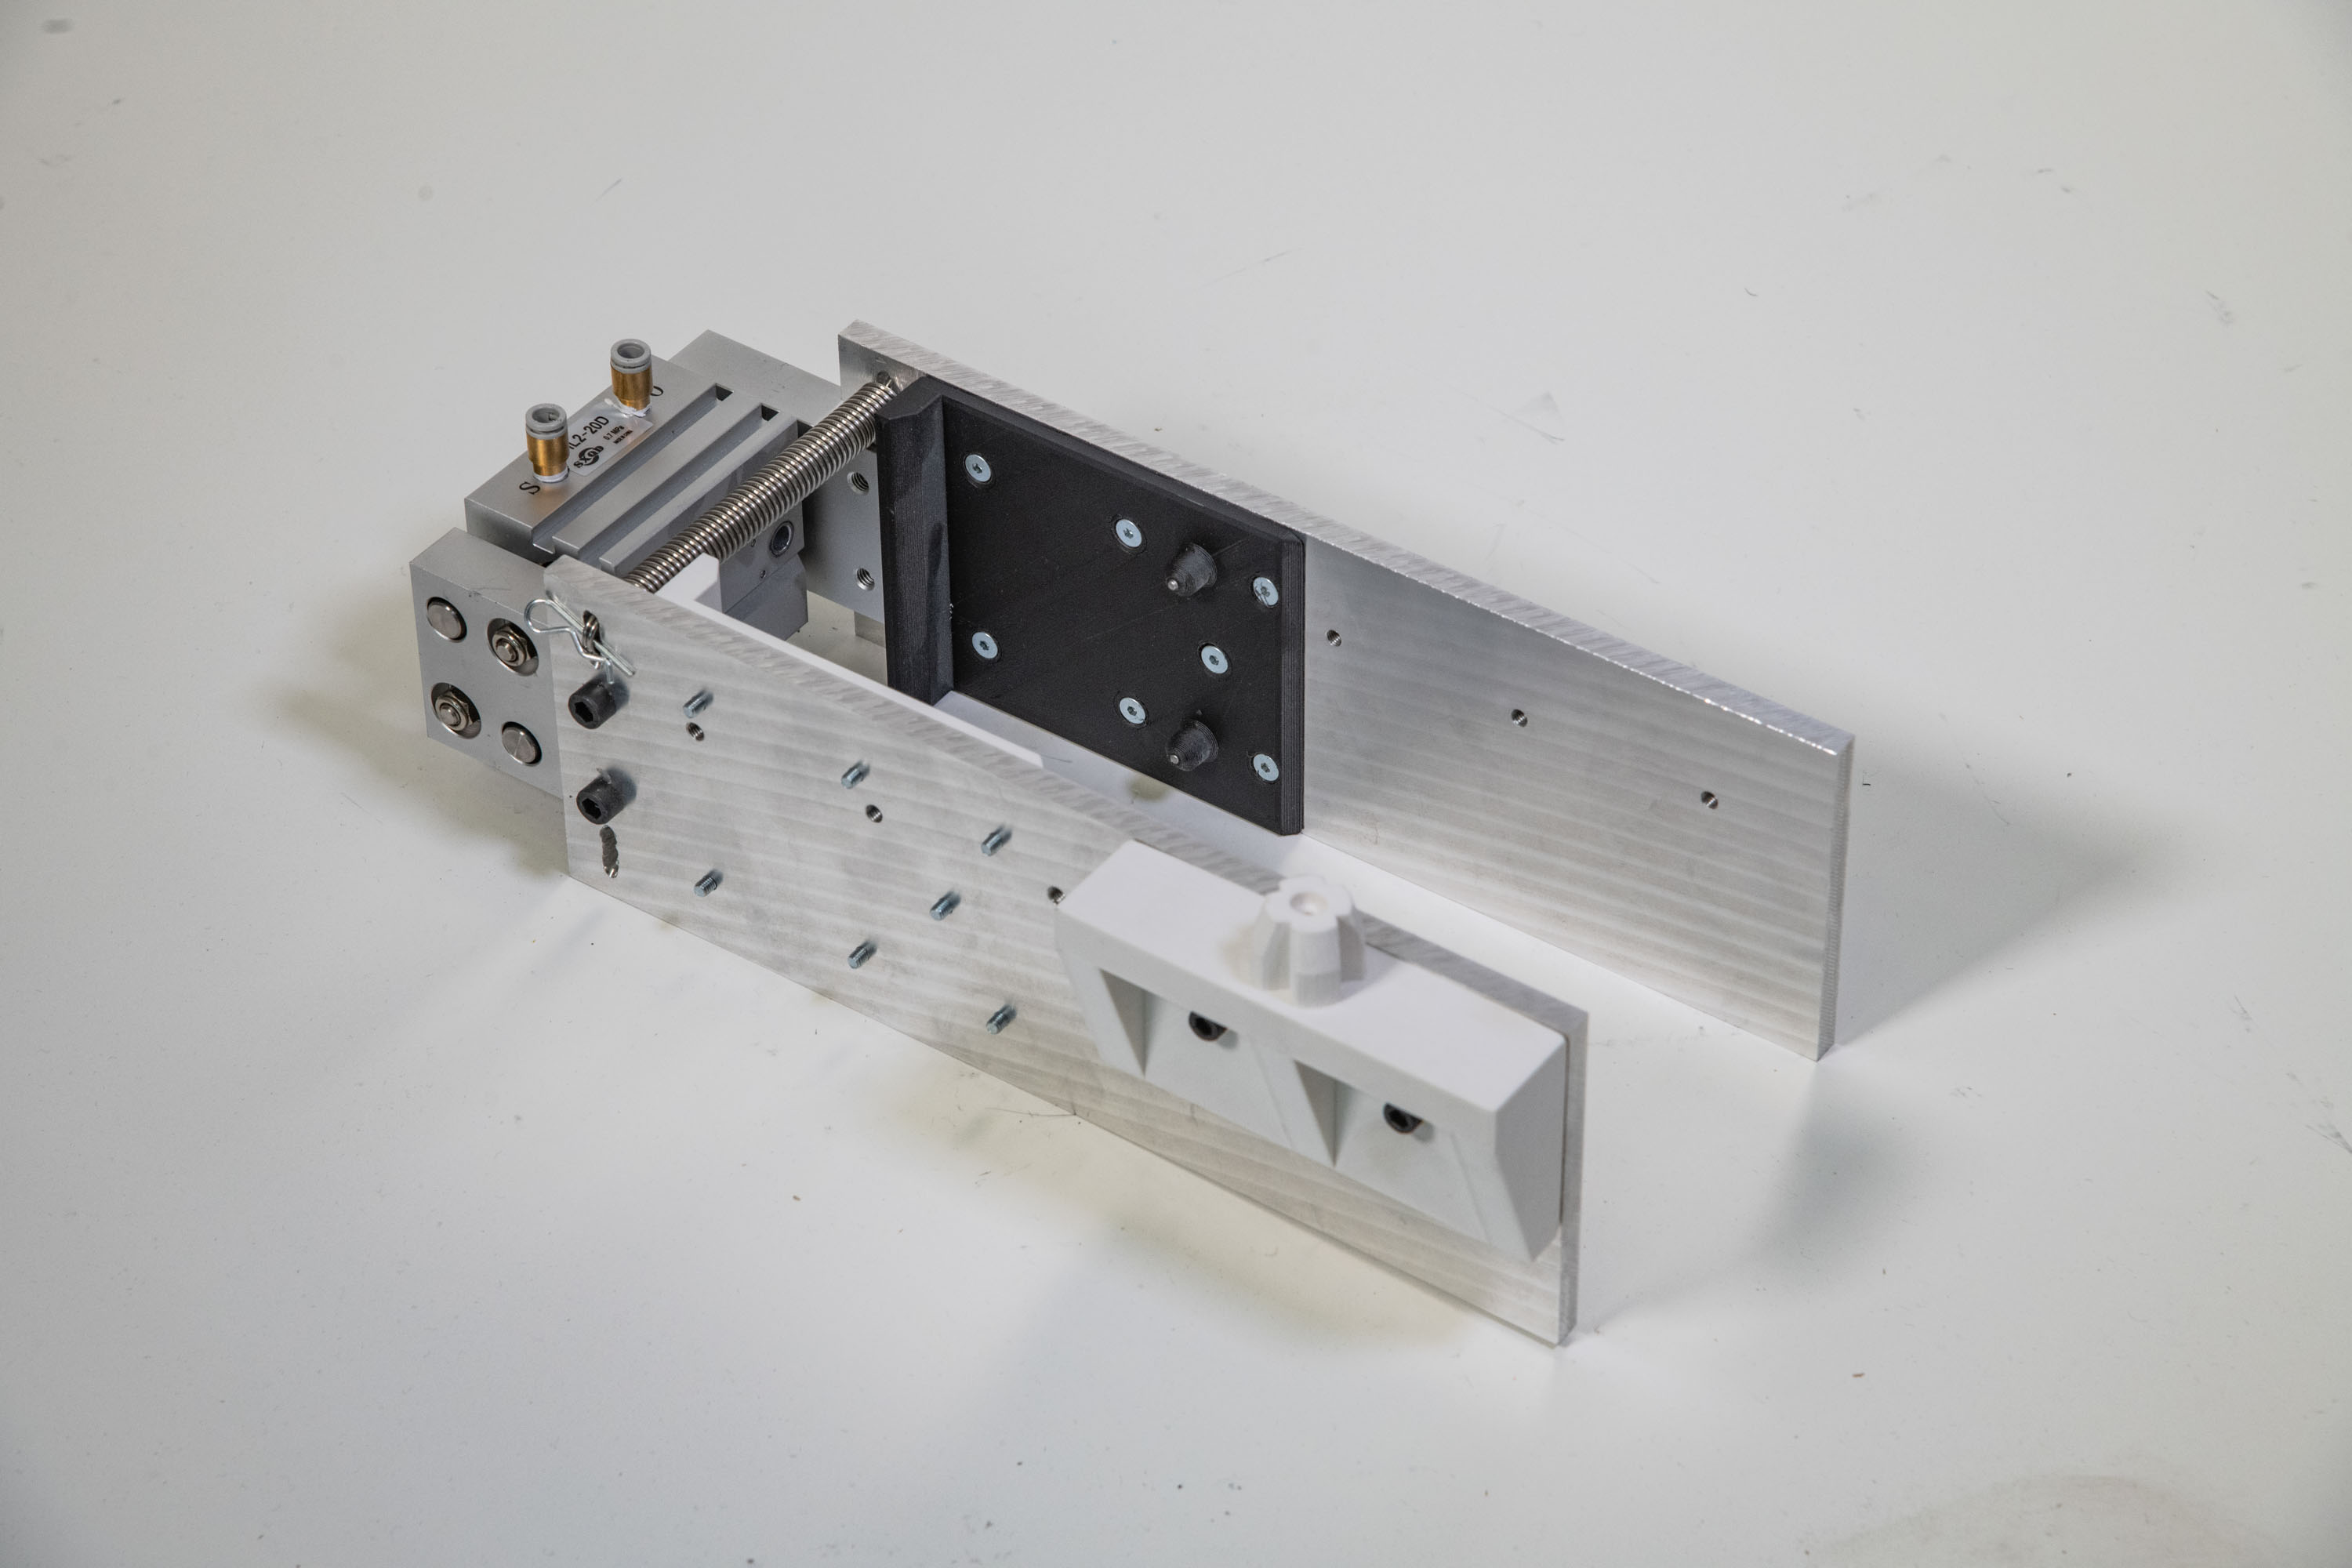
\includegraphics[width=0.99\textwidth]{images/04-3/cl1-hanging-test.jpg}
    \caption{Test setup of hanging gripper and alignment features}
    \label{fig:hanging-gripper-test}
\end{figure}

The registration holes on the beam are intended to be drilled by the automatic joinery machine. However, during this exploration round, they are drilled manually using a precision-made drilling guide (see Figure \ref{fig:drilling-jig}). This guide would be securely clamped around the 100mm x 100mm timber beam before all the necessary holes are drilled. A depth stopper was used to ensure the drilling depth. Different drilling positions can be seen on the guide used during testing and development.

\begin{figure}[h!]
    \centering
    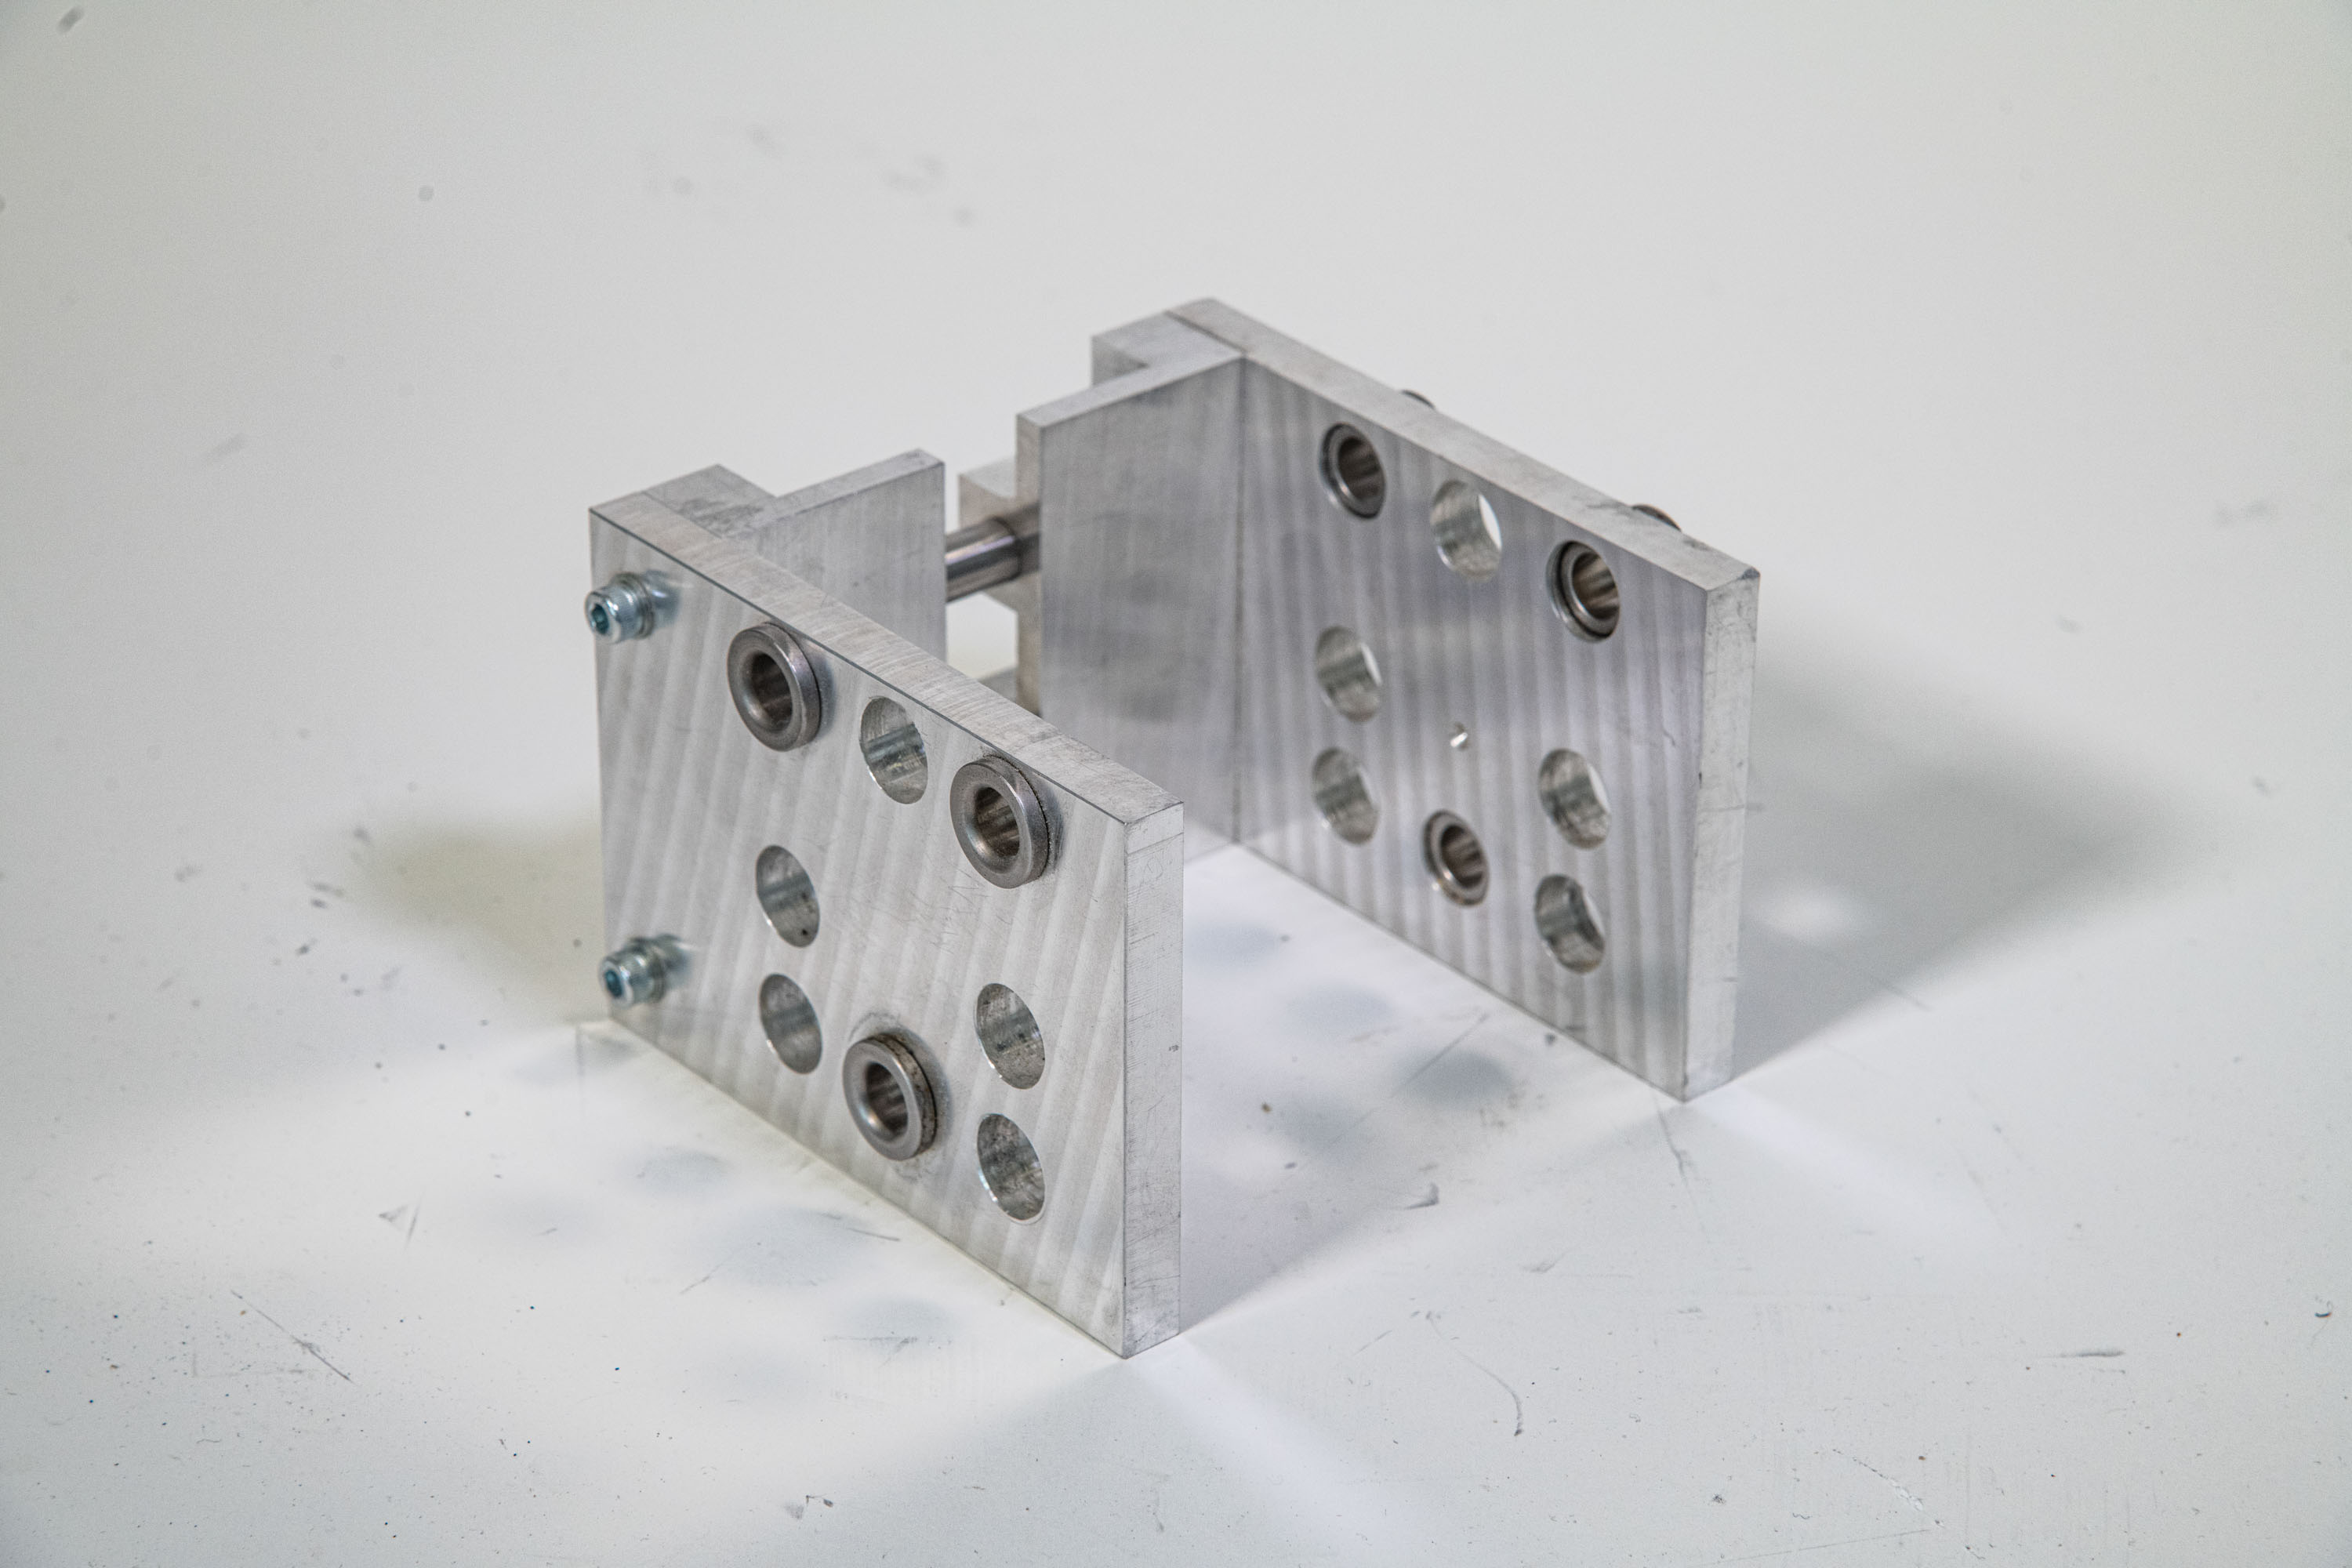
\includegraphics[width=0.99\textwidth]{images/04-3/cl1-pin-drill-jig.jpg}
    \caption{Drilling jig for drilling registration holes on the timber beam}
    \label{fig:drilling-jig}
\end{figure}



\subsubsection{Beam Rest Feature}
\label{subsubsection:exploration-1-beam-rest-feature}

The clamp is designed with a jaw that can be fitted with different plastic inserts for exploring different registration features. The features are intended to assist the alignment between the two beams. Figure \ref{fig:beam-rest-feature} show the initial design of a wedge-shaped alignment feature for guiding the beam in the horizontal direction. However, the plastic insert was never fabricated or tested because the experimental observation \seeref{subsection:exploration-1-beam-support-needed-during-clamping} has already invalidated the resting principle.

\begin{figure}[p]
    \centering
    \begin{subfigure}[b]{0.49\textwidth}
        \centering
        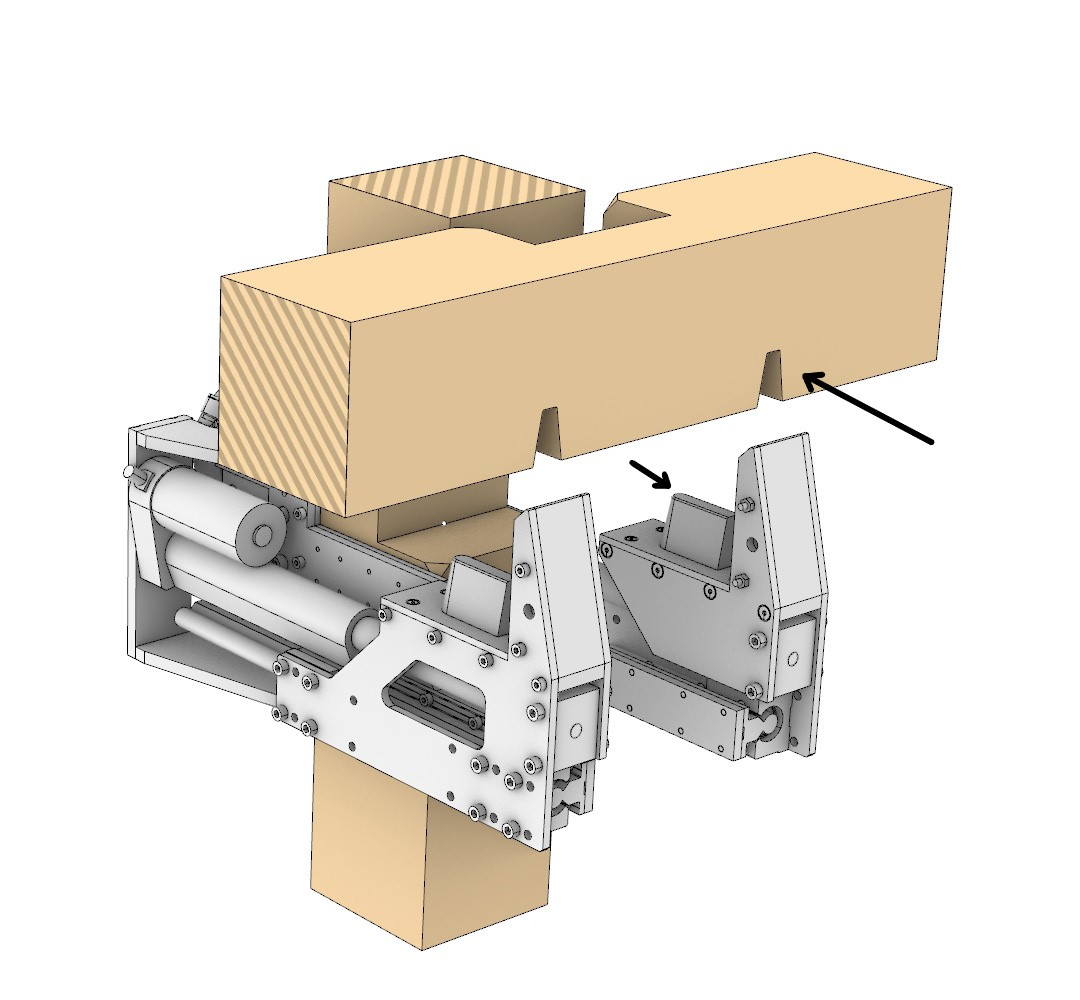
\includegraphics[width=\textwidth]{images/04-3/beam-rest-arrow.jpg}
        \caption{Beam about to be placed in clamp}
        %\label{fig:uniquesubfigurelabel}
    \end{subfigure}
    \hfill
    \begin{subfigure}[b]{0.49\textwidth}
        \centering
        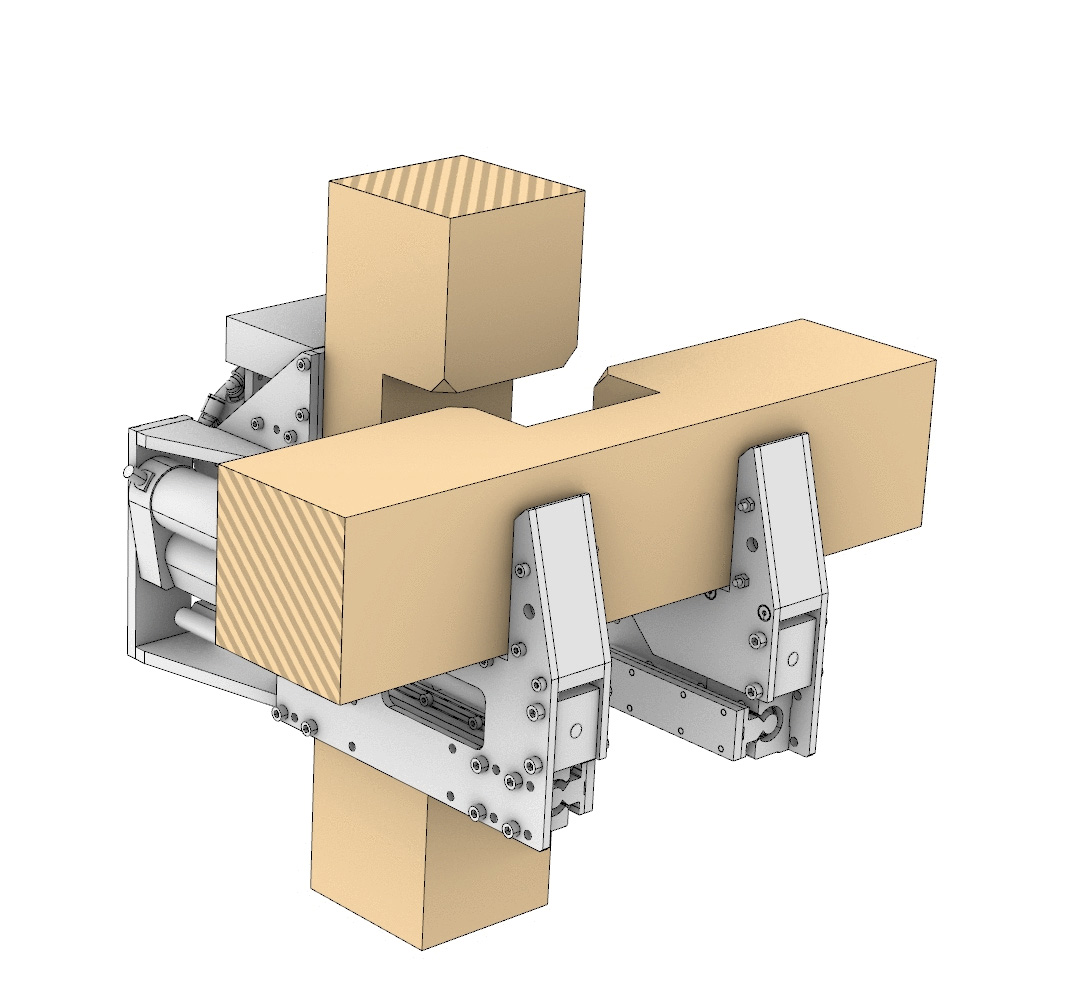
\includegraphics[width=\textwidth]{images/04-3/beam-rest2.jpg}
        \caption{Beam after being placed on the resting feature}
        %\label{fig:uniquesubfigurelabel}
    \end{subfigure}
    \caption{Sketch of a beam rest with wedge-shaped alignment feature} 
    \label{fig:beam-rest-feature}
\end{figure}


\subsubsection{Hardware Integration}
\label{subsubsection:exploration-1-hardware-integration}

The combined design of all the CL1 components can be seen in Figure \ref{fig:integrated-cl1-hardware}. The total weight of the clamp is 4.9kg. There is an intended location for the position of electronics. During the test, it was not installed at that location.

Figure \ref{fig:integrated-cl1-photo} shows the constructed CL1 clamp. Only one is made for the test. The motor cable (black) and the load cell cable (orange) can be seen leading out of the device.

Figure \ref{fig:cl1-attach-to-joint} shows how the clamp is intended to be attached to a lap joint by the robotic arm and then hanging from it. However, this clamp was never docked to the robotic arm during tests.

\begin{figure}
    \centering
    \begin{subfigure}[b]{0.49\textwidth}
        \centering
        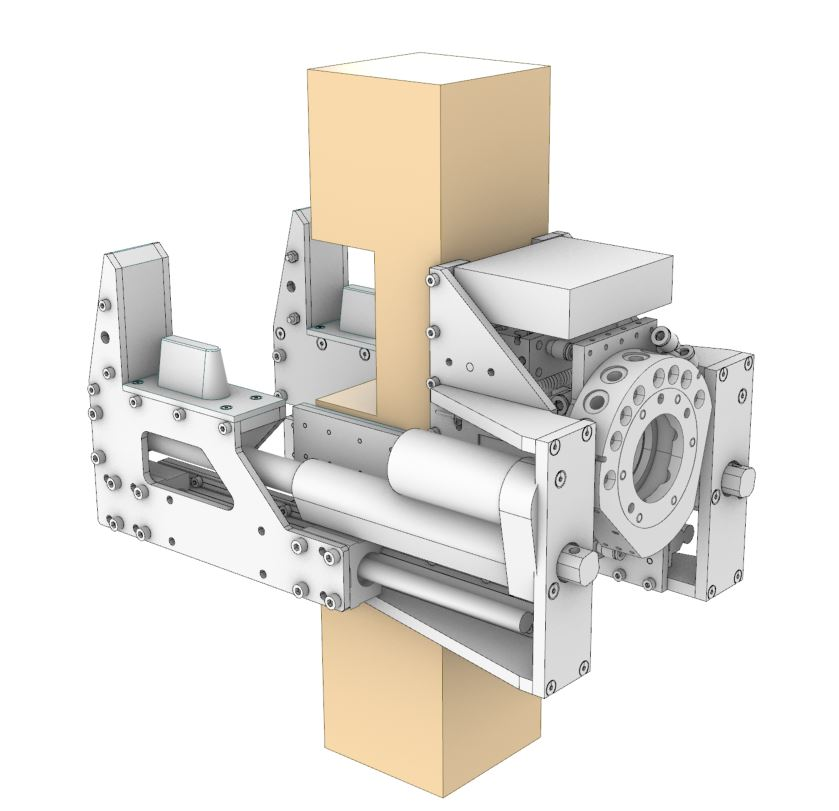
\includegraphics[width=\textwidth]{images/04-3/CL1_back.jpg}
        % \caption{Beam about to be placed in clamp}
        %\label{fig:uniquesubfigurelabel}
    \end{subfigure}
    \hfill
    \begin{subfigure}[b]{0.49\textwidth}
        \centering
        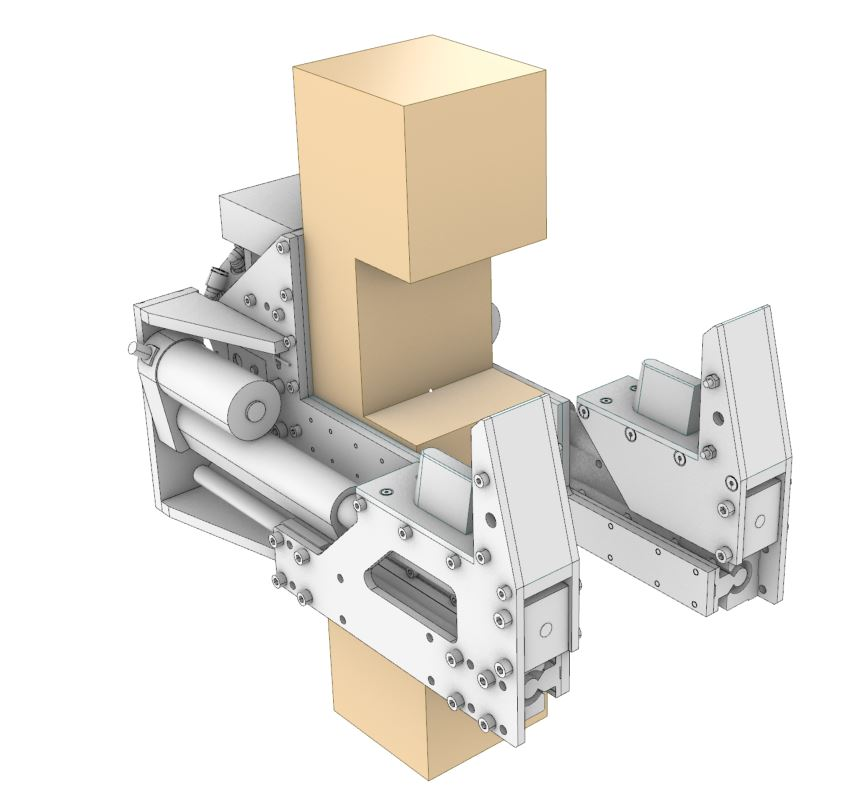
\includegraphics[width=\textwidth]{images/04-3/CL1_front.jpg}
        % \caption{Beam after being placed on the resting feature}
        %\label{fig:uniquesubfigurelabel}
    \end{subfigure}
    \caption{Integrated design of the CL1 clamp} 
    \label{fig:integrated-cl1-hardware}
\end{figure}

\begin{figure}
    \centering
    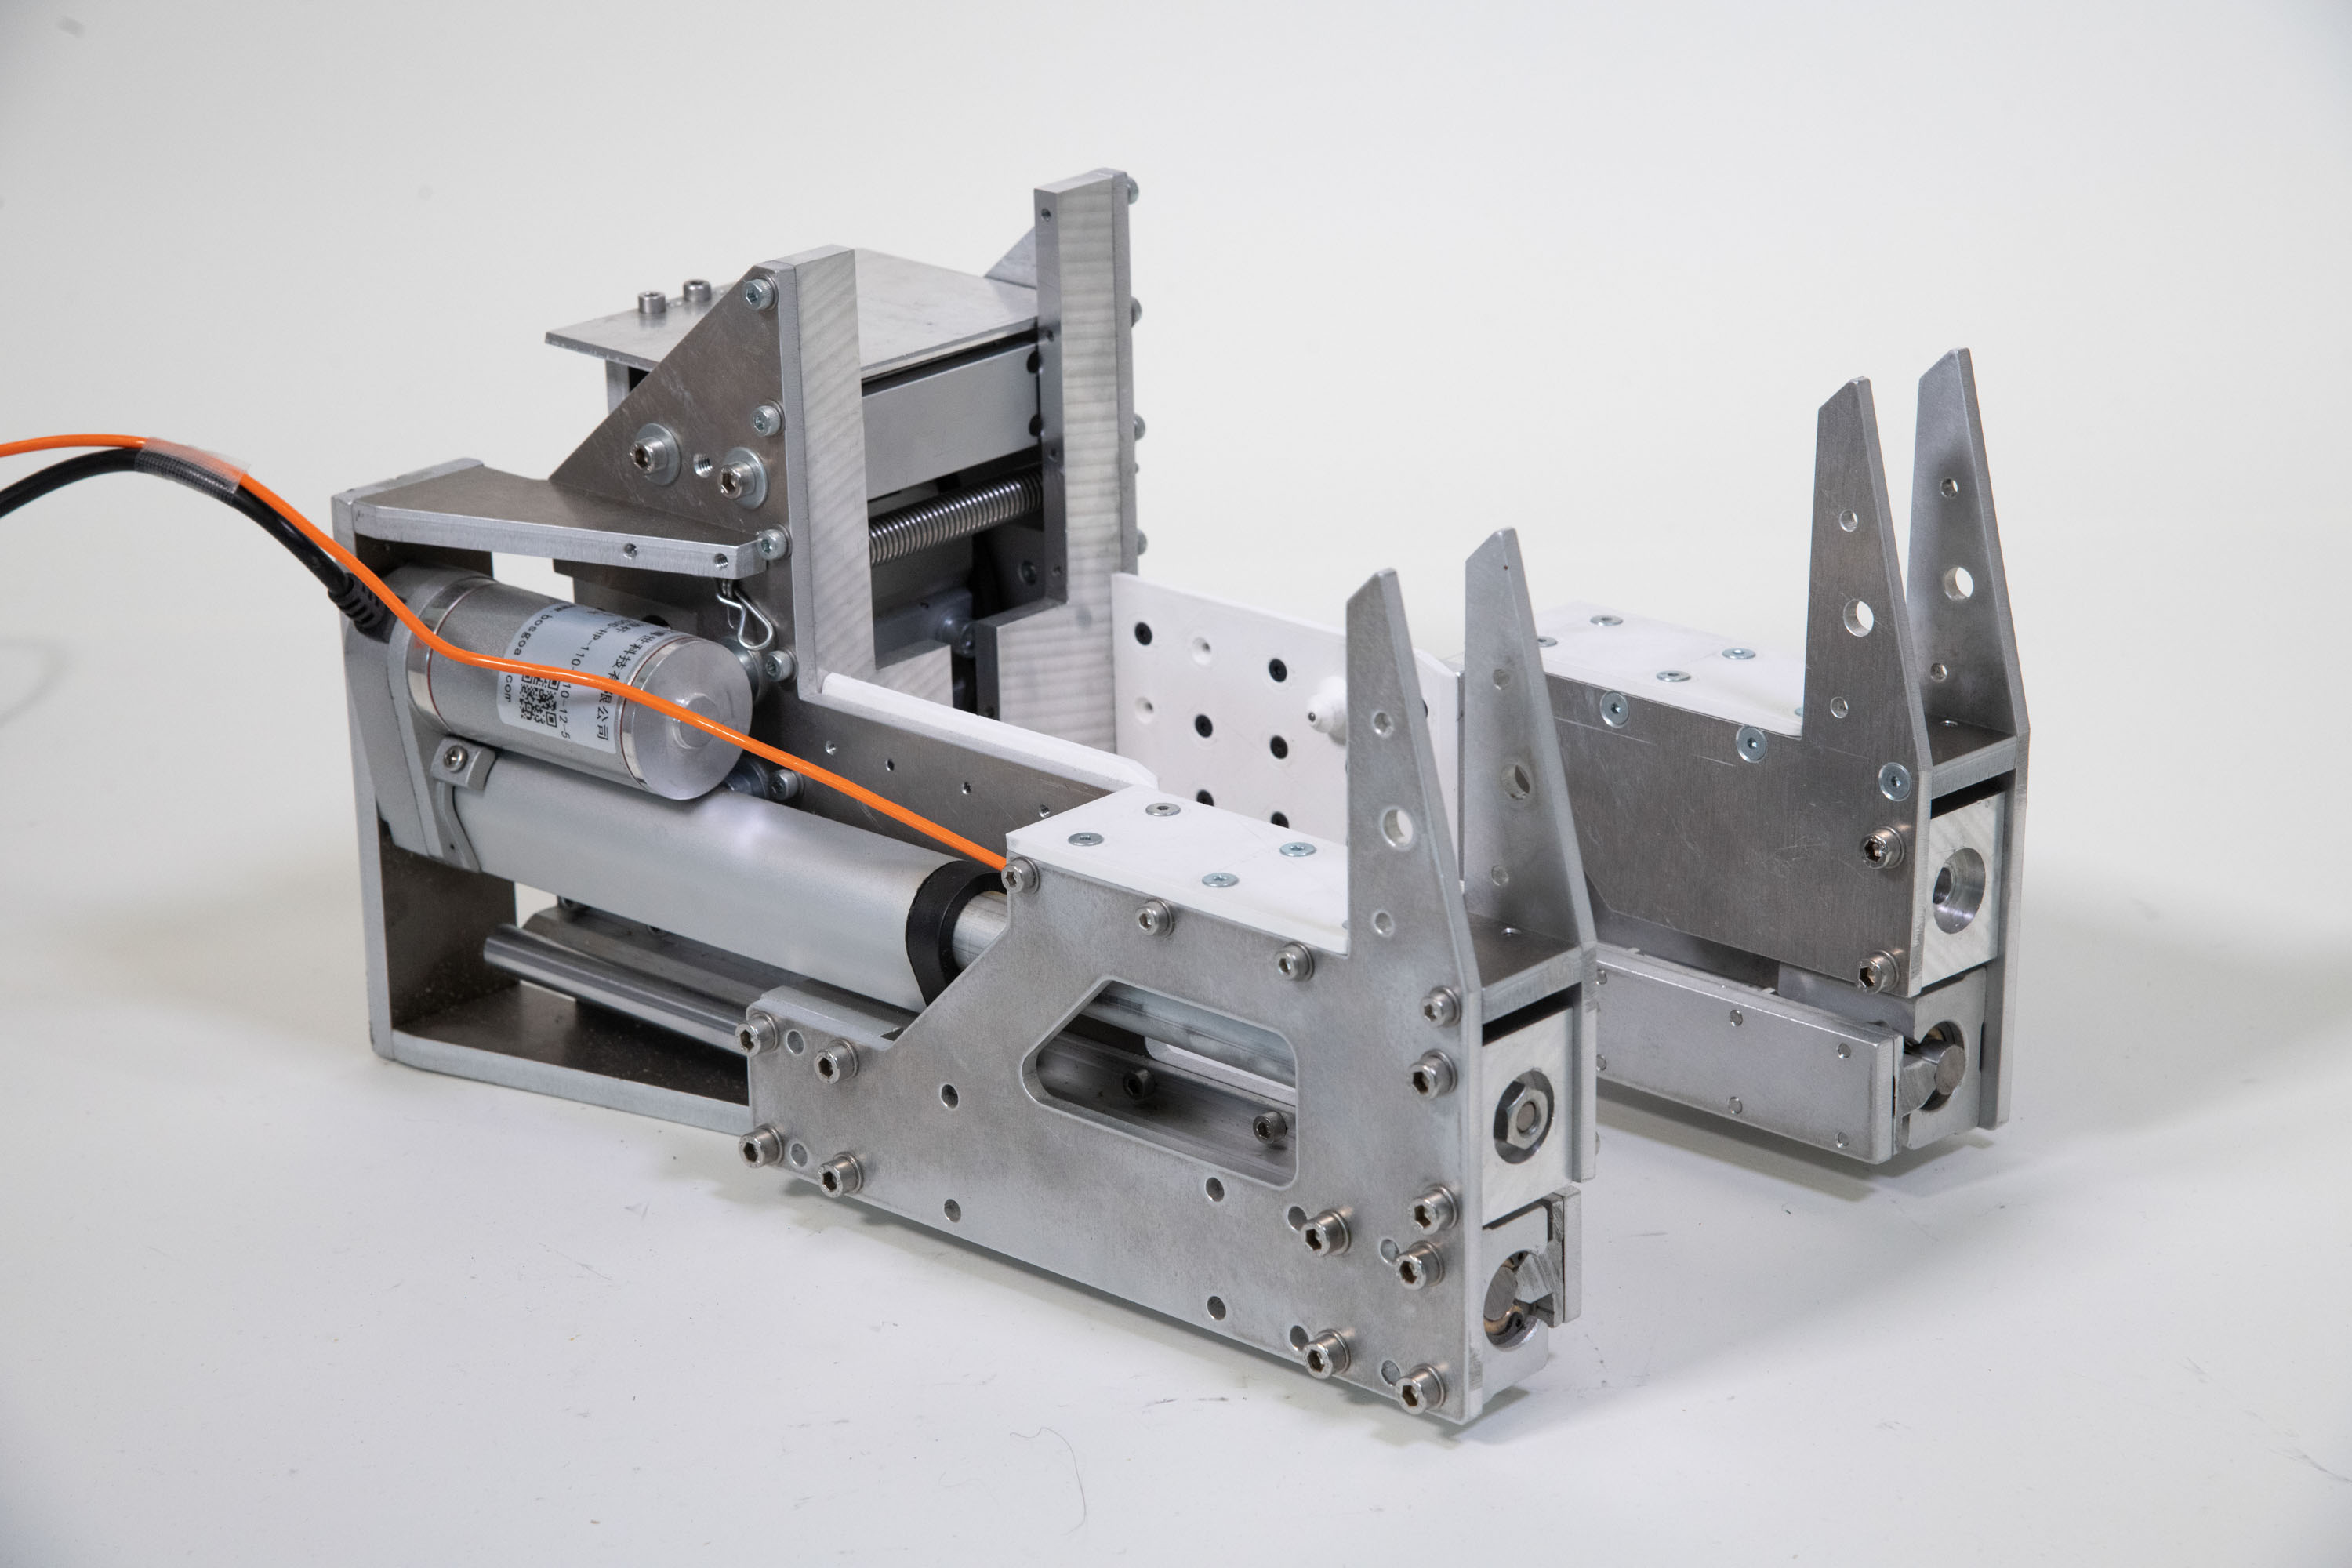
\includegraphics[width=0.99\textwidth]{images/04-3/cl1-completed.jpg}
    \caption{Drilling jig for drilling registration holes on the timber beam}
    \label{fig:integrated-cl1-photo}
\end{figure}

\begin{figure}
    \centering
    \begin{subfigure}[b]{0.90\textwidth}
        \centering
        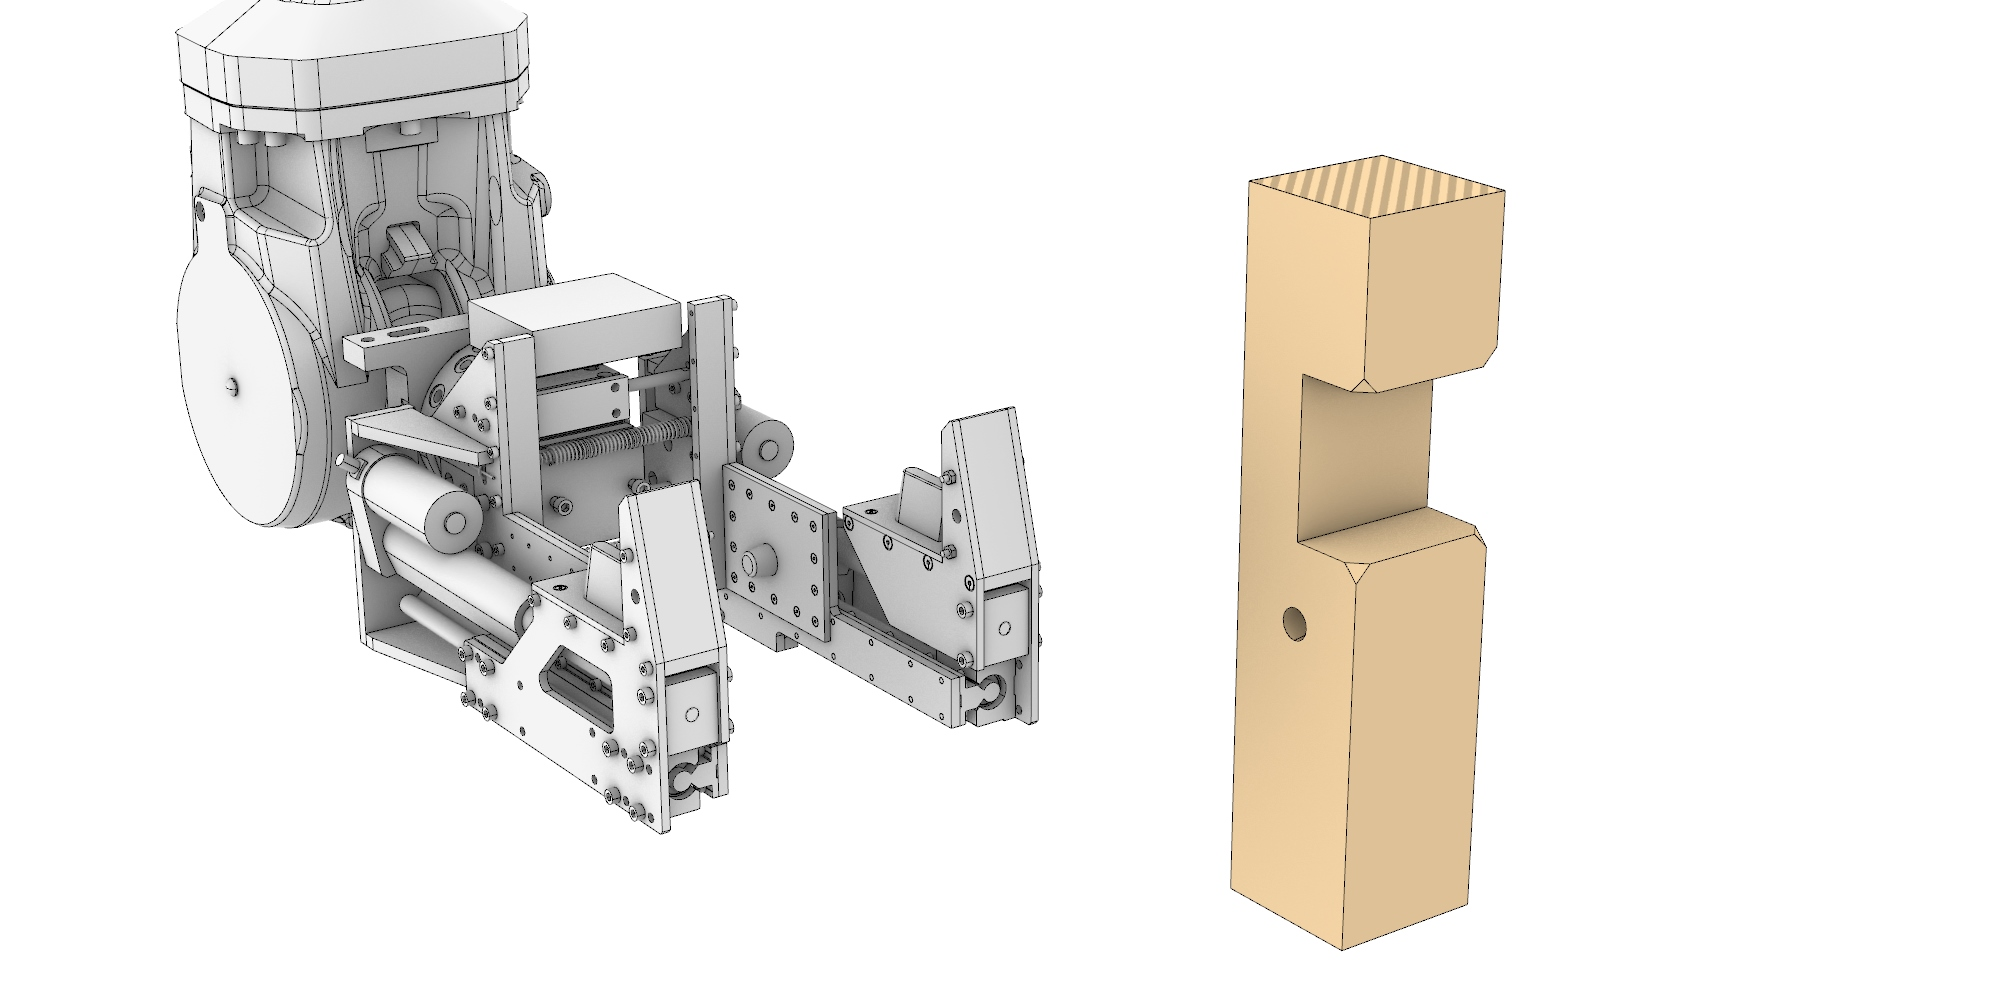
\includegraphics[width=\textwidth]{images/04-3/Attach_1.jpg}
        % \caption{SubFigureCaption}
        %\label{fig:uniquesubfigurelabel}
    \end{subfigure}
    \vskip\baselineskip % Next row

    \begin{subfigure}[b]{0.90\textwidth}
        \centering
        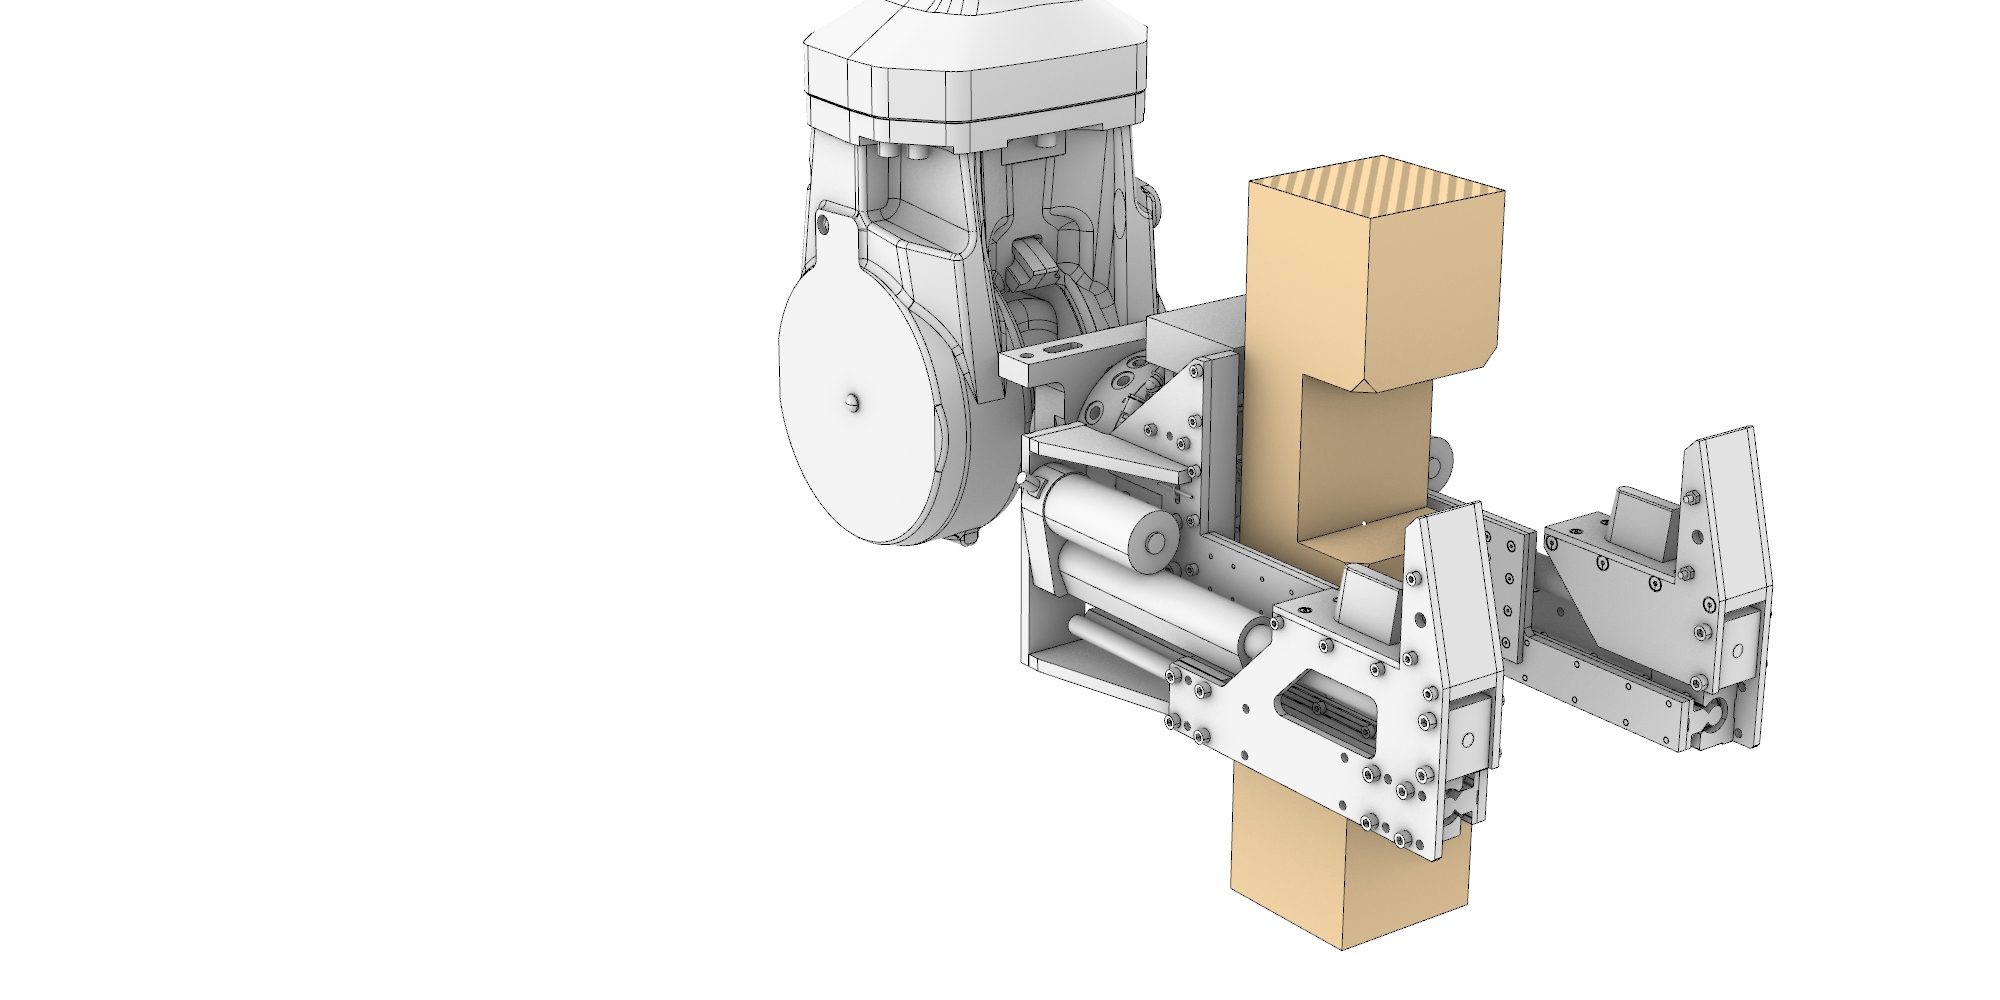
\includegraphics[width=\textwidth]{images/04-3/Attach_7.jpg}
        % \caption{SubFigureCaption}
        %\label{fig:uniquesubfigurelabel}
    \end{subfigure}
    \vskip\baselineskip % Next row

    \begin{subfigure}[b]{0.90\textwidth}
        \centering
        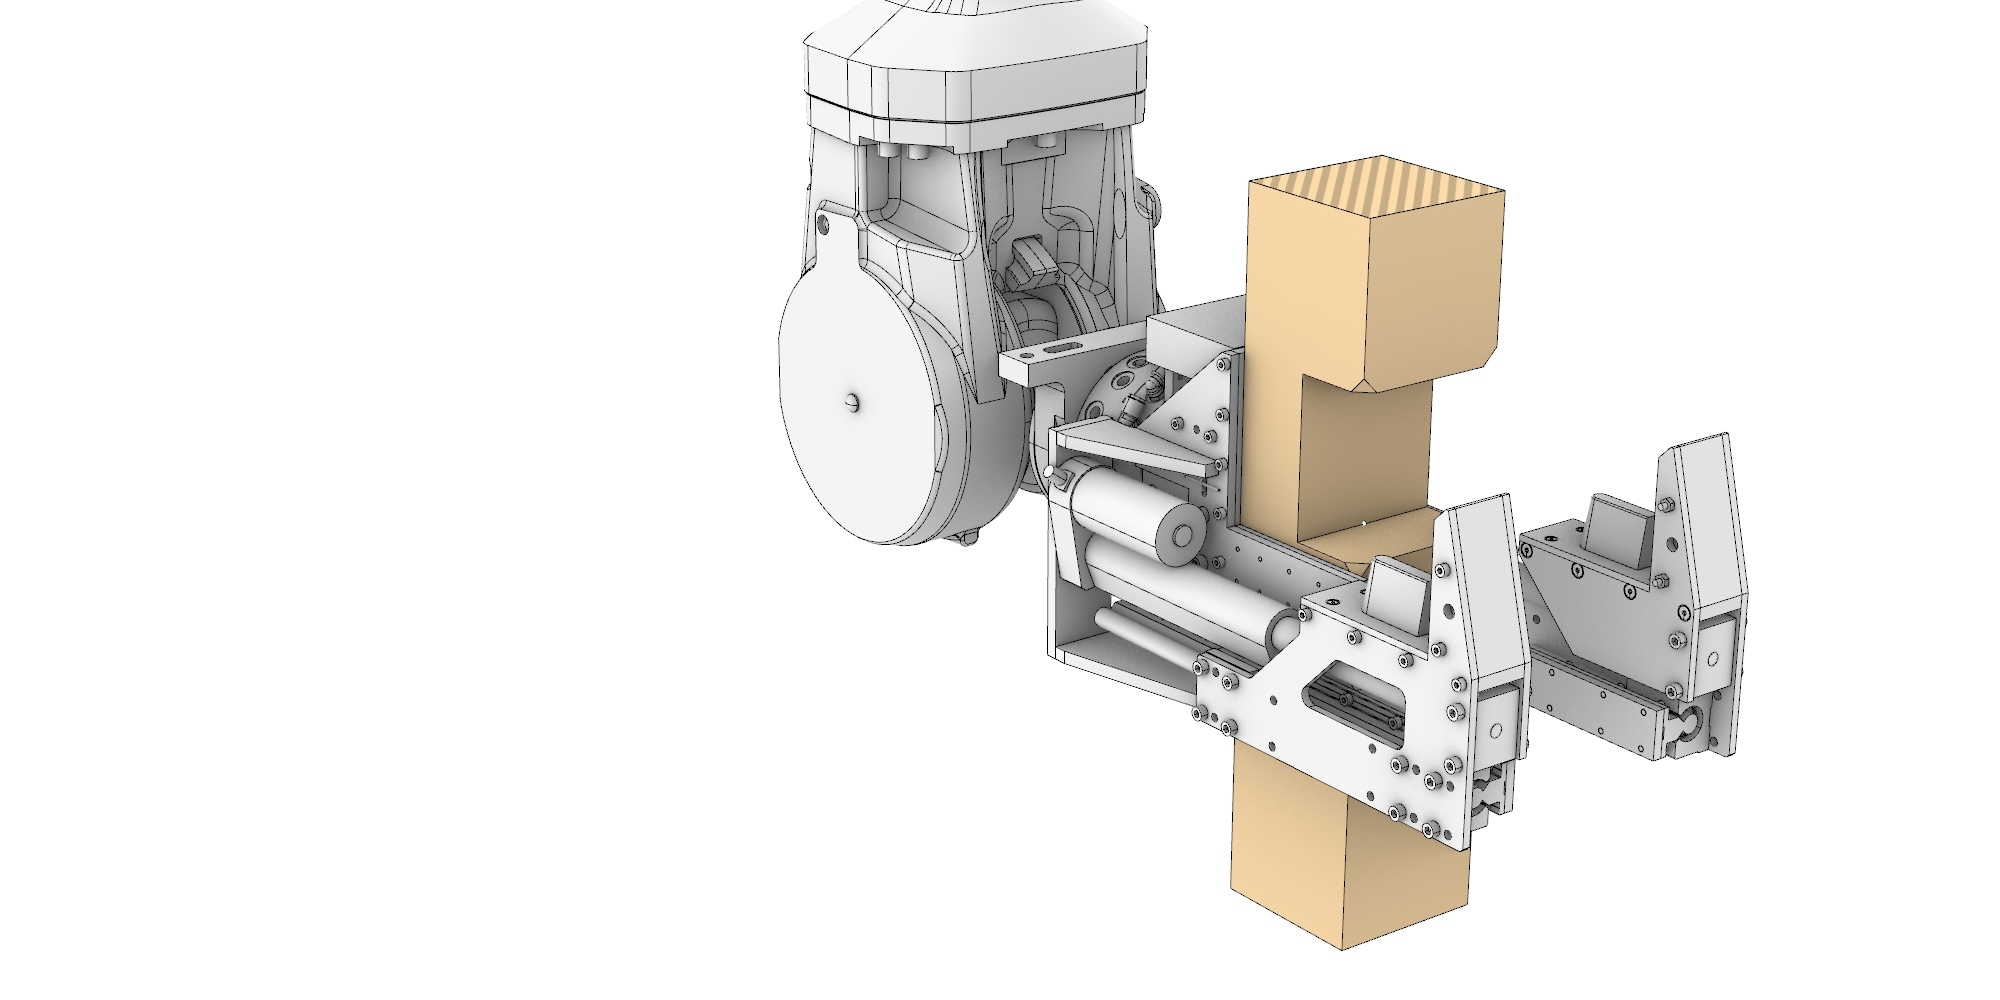
\includegraphics[width=\textwidth]{images/04-3/Attach_11.jpg}
        % \caption{SubFigureCaption}
        %\label{fig:uniquesubfigurelabel}
    \end{subfigure}

    \caption{Diagram sequence showing how the clamp is attached to a lap joint}
    \label{fig:cl1-attach-to-joint}
\end{figure}

\subsection{CL1 Clamp Drive System}
\label{subsection:exploration-1-cl1-clamp-electronics}

Being the first DiRT electronic controller, the CL1 Clamp controller was designed together with the creation of the motor control algorithms, which had a large influence on the choice of components. The initial goal of the electronics development is to identify a combination of control algorithms, choice of motor, encoder, and motor driver that allows controlled movement of the two motors following a predefined trajectory.
After the initial goal is successful, the setup is also added with other features as part of a validation test to confirm major systems:

\begin{itemize}[nosep]
    \item LiPo battery power input for motor driver
    \item Regulation of battery voltage for controller logic voltage
    \item Wireless communication using radio module
\end{itemize}

\subsubsection{System Voltage}
\label{subsubsection:exploration-1-system-voltage}

The development started by identifying the system voltage, which depended on the choice of battery and actuator motor. In order to maximise the power available in short-burst output, I decided the best battery chemistry choice is Lithium Polymer (LiPo) because of its high power density. Table \ref{table:common-lipo-properties} listed some of LiPo properties at the time of writing:

\begin{table}[]
    \includegraphics[page=3, trim=25.4mm 210mm 25.4mm 33mm, clip, width=\textwidth]{tables/Tables in Chapter 4.pdf}
    \caption{Common lithium polymer battery properties}
    \label{table:common-lipo-properties}
\end{table}

Considering that most of the common DC motors are either 12V or 24V, I decided the best motor and battery combination would be a 12V motor with a 4S battery. The battery voltage can range between 12.8V (discharged) and 16.8V (fully charged), which leaves some margin for voltage drop during operation and can be throttled by PWM control over the driver if necessary. The selected linear actuator also runs on 12V \seeref{subsubsection:exploration-1-linear-actuator-and-jaw-design}.

\subsubsection{Motor Driver}
\label{subsubsection:exploration-1-motor-driver}

The choice of motor driver is a Dual H-Bridge Motor Controller (XY160D manufactured by Handson Technology) (See Table \ref{table:hbridge-xz160d-properties} for its specifications) which weighted only 32 grams. The H-Bridge configuration allows bi-directional DC motor control that is necessary for clamp jaw retraction and extension. This type of H-Bridge motor driver is very common and is made by many different companies with different current ratings. The intention of choosing this type of driver is to facilitate future upgrades if necessary. 

\begin{table}[]
    \includegraphics[page=4, trim=25.4mm 210mm 25.4mm 33mm, clip, width=\textwidth]{tables/Tables in Chapter 4.pdf}
    \caption{Properties of the Dual H-Bridge Motor Controller XY160D}
    \label{table:hbridge-xz160d-properties}
\end{table}

The motor driver supports four possible control modes (see Table \ref{table:hbridge-xz160d-control-logic}). Its control logic is a common scheme that is made famous by the L298 motor driver chip and is commonly found on motor drivers. There are three digital signal inputs, IN1, IN2, and ENA. ENA represents motor enable, which can be supplied with a PWM signal to throttle the motor.

\begin{table}[]
    \includegraphics[page=5, trim=25.4mm 210mm 25.4mm 33mm, clip, width=\textwidth]{tables/Tables in Chapter 4.pdf}
    \caption{Control logic of Motor Controller XY160D}
    \label{table:hbridge-xz160d-control-logic}
\end{table}

\subsubsection{LiPo Battery}
\label{subsubsection:exploration-1-lipo-battery}

Based on the specification of the chosen linear actuator, the 12V option is rated at 60W with 5mm/s at 2000N output. It will draw 5A at constant maximum power, which should be compatible with this 7A driver. It will take approximately 20 seconds to traverse 120mm, assuming 80\% driver efficiency, each full stroke which will consume about 35mAh. A complete cycle of clamping and retraction can consume roughly 70mAh. Based on this rough calculation, a 1000mAh battery was chosen, as it will support approximately 10 cycles, assuming the battery has only 80\%-90\% usable capacity.   
Table \ref{table:lipo-battery-survey} listed some of the 4S LiPo batteries on the market as of April 2023. 

\begin{table}[]
    \includegraphics[page=6, trim=25.4mm 210mm 25.4mm 33mm, clip, width=\textwidth]{tables/Tables in Chapter 4.pdf}
    \caption{Survey of 4S LiPo batteries on the market}
    \label{table:lipo-battery-survey}
\end{table}

Different capacities were tested with no major performance difference being observed, the only difference is that larger capacity would provide more operation cycles between recharge.

\subsubsection{Microcontroller}
\label{subsubsection:exploration-1-microcontroller}

The Arduino family of microcontroller boards was selected for this development due to their extensive library support for integrated and external hardware. 
\textbf{Arduino Uno} was chosen for initial tests development, the reason being:

\begin{itemize}[nosep]
    \item Low cost and widespread availability.
    \item Presence of two external interrupt signal inputs, making it suitable for counting motor encoder output. 
    \item Integrated USB serial communication, which greatly simplifies debugging and control.
    \item Equipped with an ATmega328 CPU running at 16 MHz, these Arduino boards are popular choices for embedded motion control tasks.
\end{itemize}

The Arduino Uno is later switched to \textbf{Arduino Nano}, which has the same functionality but a smaller form factor. The following General Purpose Input Output (GPIO) pins are used:

\begin{itemize}[nosep]
    \item The motor drivers require three digital signals, one of which requires PWM output, for controlling each motor channel. The two channels occupied 6 pins. 
    \item There are two encoder channels from each motor, one of which is connected to the external interrupt pin. In total, both motor encoders occupied 4 pins.
    \item There are provisions for connecting to the CC1101 radio module and two load cells. This was tested during development but was not implemented for the demonstration. The integration with the radio module is continued in the next Exploration Round.
    \item One of the Analog-to-Digital Converter (ADC) input pins is used for monitoring battery voltage.
\end{itemize}

In order to monitor battery voltage, it is connected to the ADC over a voltage divider with a ratio of 3.35 to 1 (see the schematic below). A fully charged LiPo 4S battery at 16.8V will be reduced to 5.01V, which coincides with the upper bound of the ADC. The ADC has 10 bit resolution (1024 steps) or 0.00488V per step \\($5.0V / 1024 steps$). This circuit design will provide an effective resolution ($R_{Eff}$) between a full battery at 16.8V and an empty battery at 12.8V : 
\\ $R_{Eff} = (16.8V - 12.8V) / 0.00488V = 243 steps$

The \textit{Measured Voltage} is related to the \textit{Raw Values} (obtained from the ADC) by a divisor variable and an offset variable. Values of which has to be calibrated after construction for each device to compensate for component deviations. 

\paragraph{Validation}

The Motor Driver and the Arduino Uno were validated in a test setup before the development of the schematics. The test confirmed:
\begin{itemize}
    \item Bi-direction control of the actuator using the driver
    \item Encoder output can be read using the interrupt pins
    \item Motion and driver operation under 12V power, without PWM throttle
\end{itemize}

\subsubsection{Voltage Regulation}
\label{subsubsection:exploration-1-voltage-regulation}

During remote-controlled operation, the 16.8V battery power had to be regulated to 5V for the Arduino microcontroller. A simple linear regulation circuitry based on LM7805 was used for the regulation. Due to the large voltage drop (11.8V), the efficiency of the regulation was expected to be low. However, the low current drawn from the microcontroller (19 mA) and the encoders (4 mA) should not create a power and heat dissipation problem.

The following calculation was performed using ambient temperature $T_A = 25^{\circ}C$. The thermal resistance of the TO-220 package $\theta_{JA} = 19^{\circ}C/W$. Without a heatsink, the package-to-ambient is approximately $70 ^{\circ}C/W$.

Power Dissipation $P_D = (V_{in} - V_{out}) * I_{out} = (11.8V) \times 23mA = 271mW$

Using the thermal formula obtained from LM7805 spec sheet, the junction temperature of the chip $T_J$ can be computed. The result is that the junction temperature is far below the maximum junction temperature $T_J{max} = 150^{\circ}C$.

\begin{align}
    P_D &= (T_J - T_A) / \theta_{JA}\nonumber \\
    0.271W &= (T_J - 25^{\circ}C) / (19^{\circ}C/W + 70^{\circ}C/W)\nonumber \\
    T_J &= 49.1^{\circ}C\nonumber
\end{align}

\subsubsection{Schematics}
\label{subsubsection:exploration-1-schematics}

The schematic of the controller is shown in Figure \ref{fig:schematic-cl1-controller}, including the assignment of pins on the Arduino controller.

\begin{figure}
    \centering
    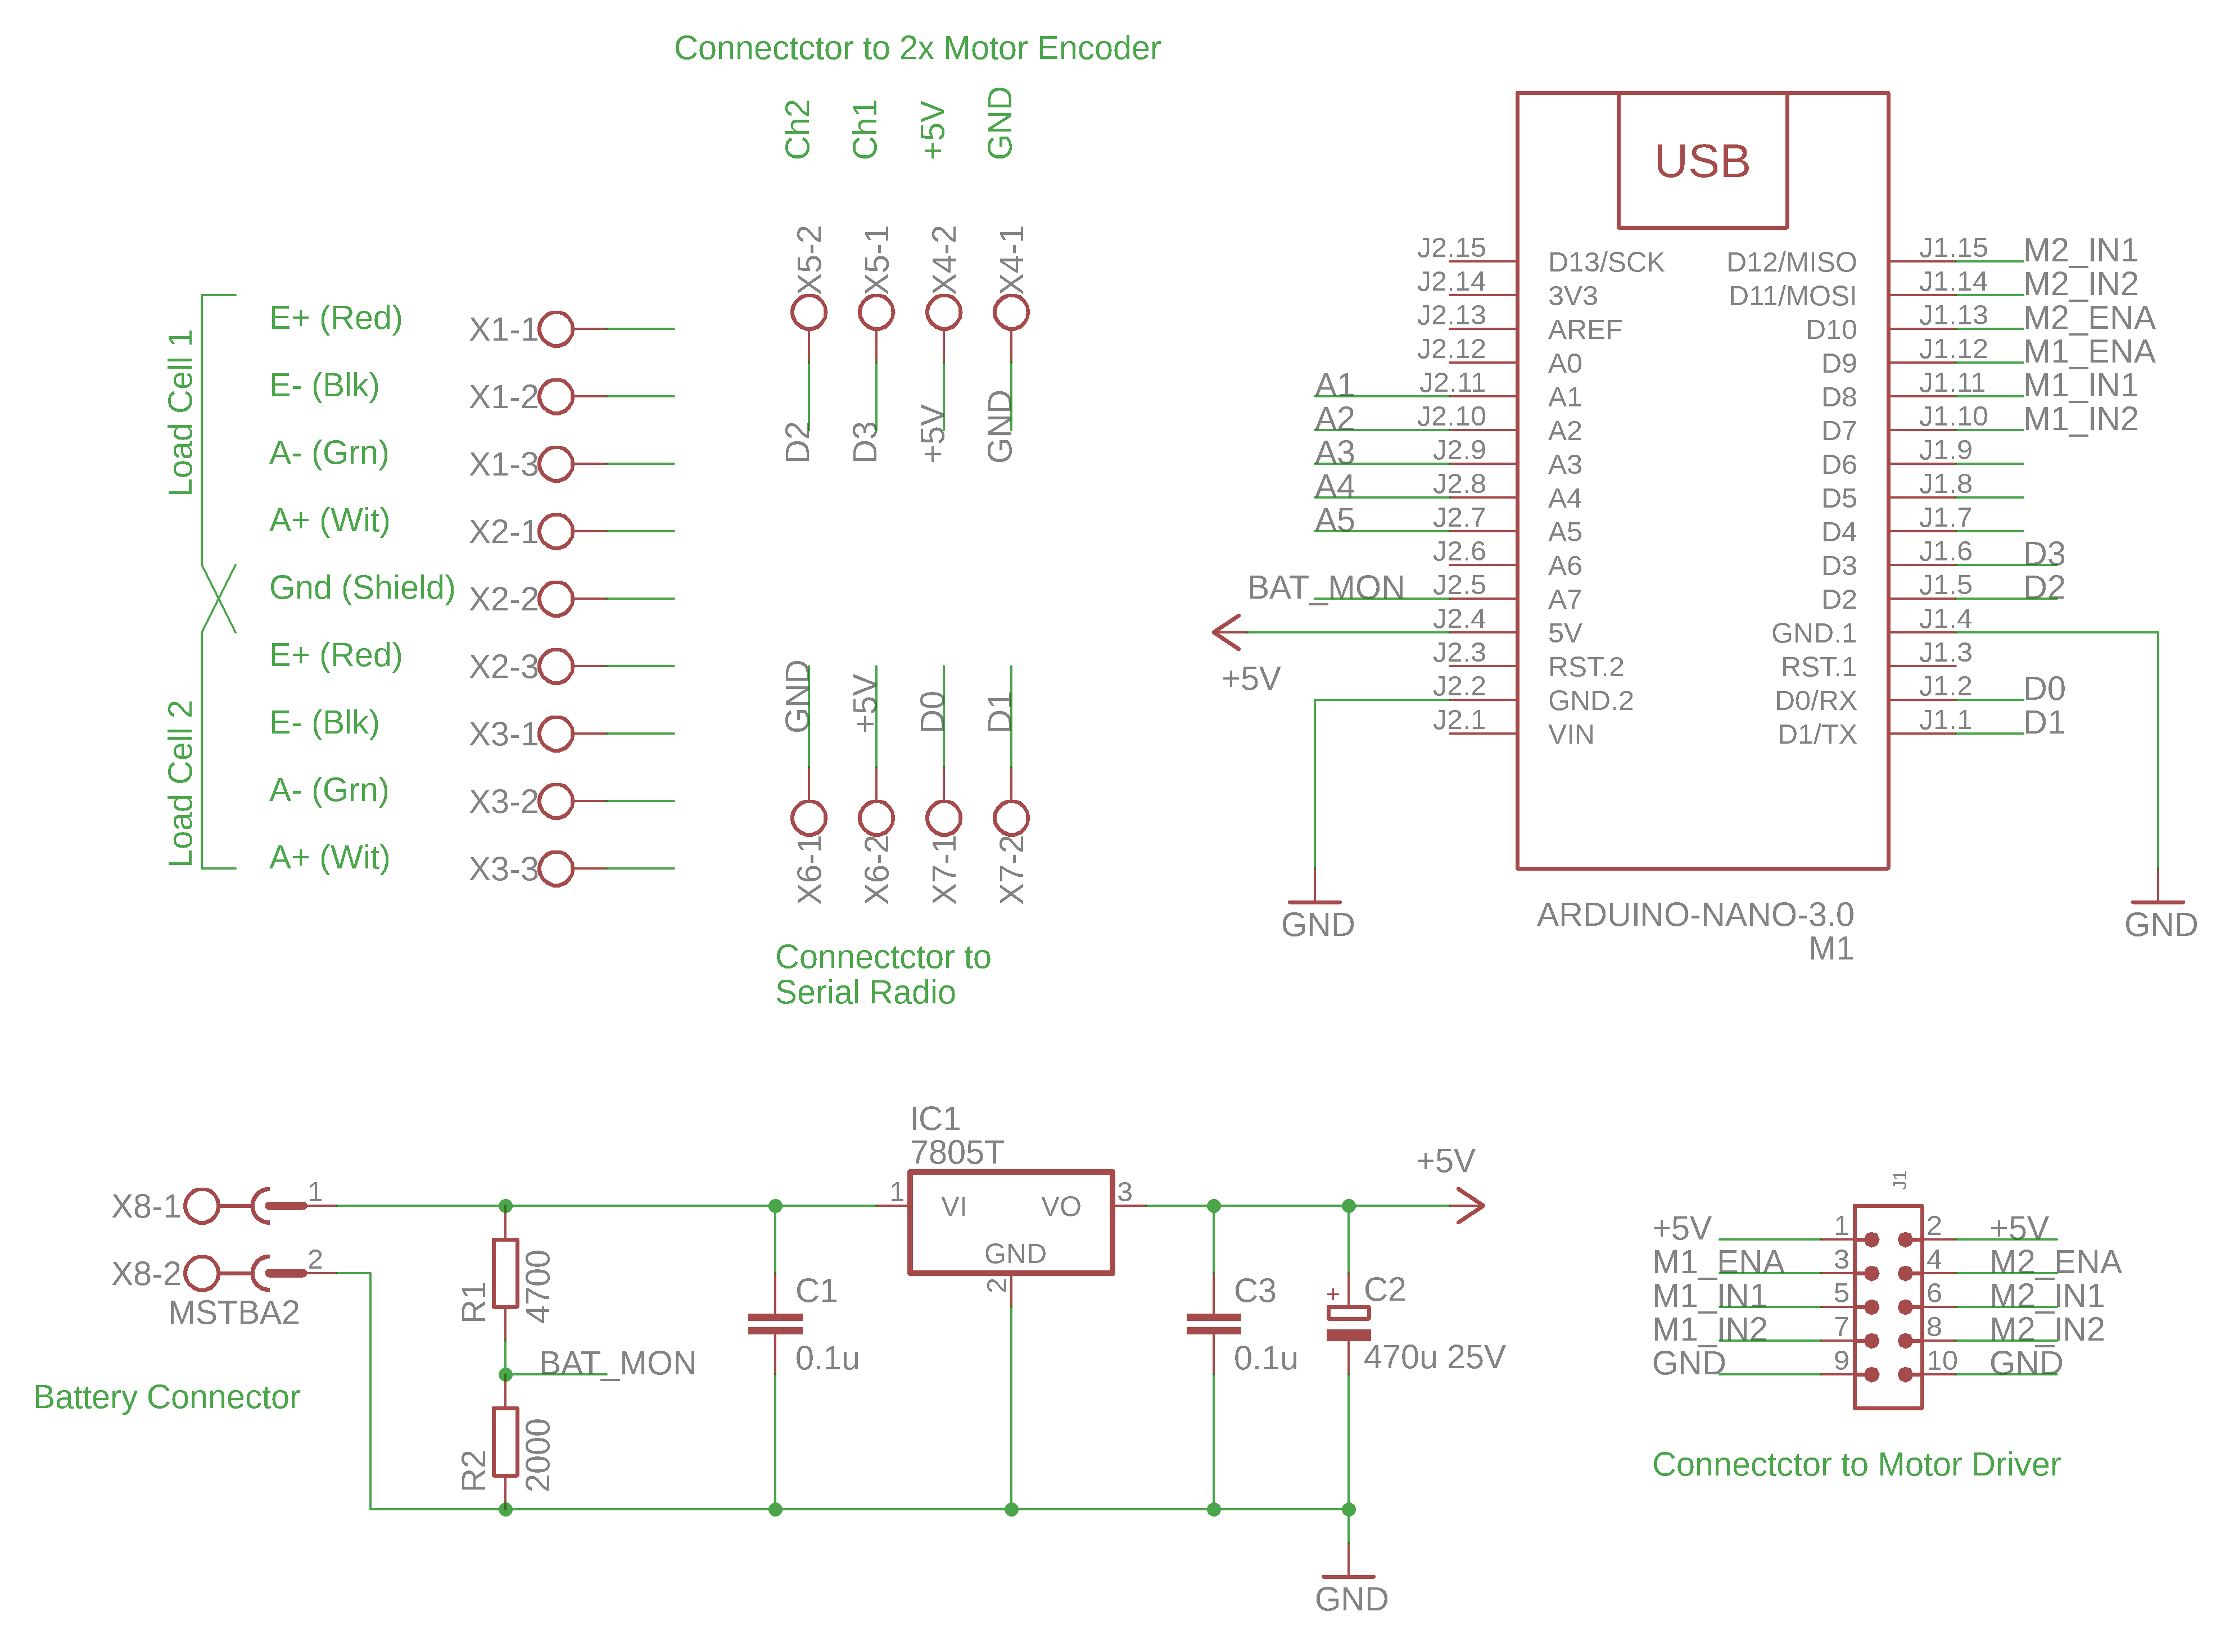
\includegraphics[width=0.90\textwidth]{images/04-3/SerialController_Schematic.png}
    \caption{Schematic of the CL1 Clamp Controller}
    \label{fig:schematic-cl1-controller}
\end{figure}


\subsubsection{Construction}
\label{subsubsection:exploration-1-construction}

Only one copy of this design was constructed for the test (see Figure \ref{fig:photo-cl1-controller}). It was soldered on a 50mm x 70mm protoboard with a female pin header connector for stacking it above the motor driver module (red). All connections were wired manually with small wires. The four wires with green plugs were intended for connecting to a future wireless communication module. However, it was never tested.

\begin{figure}
    \centering
    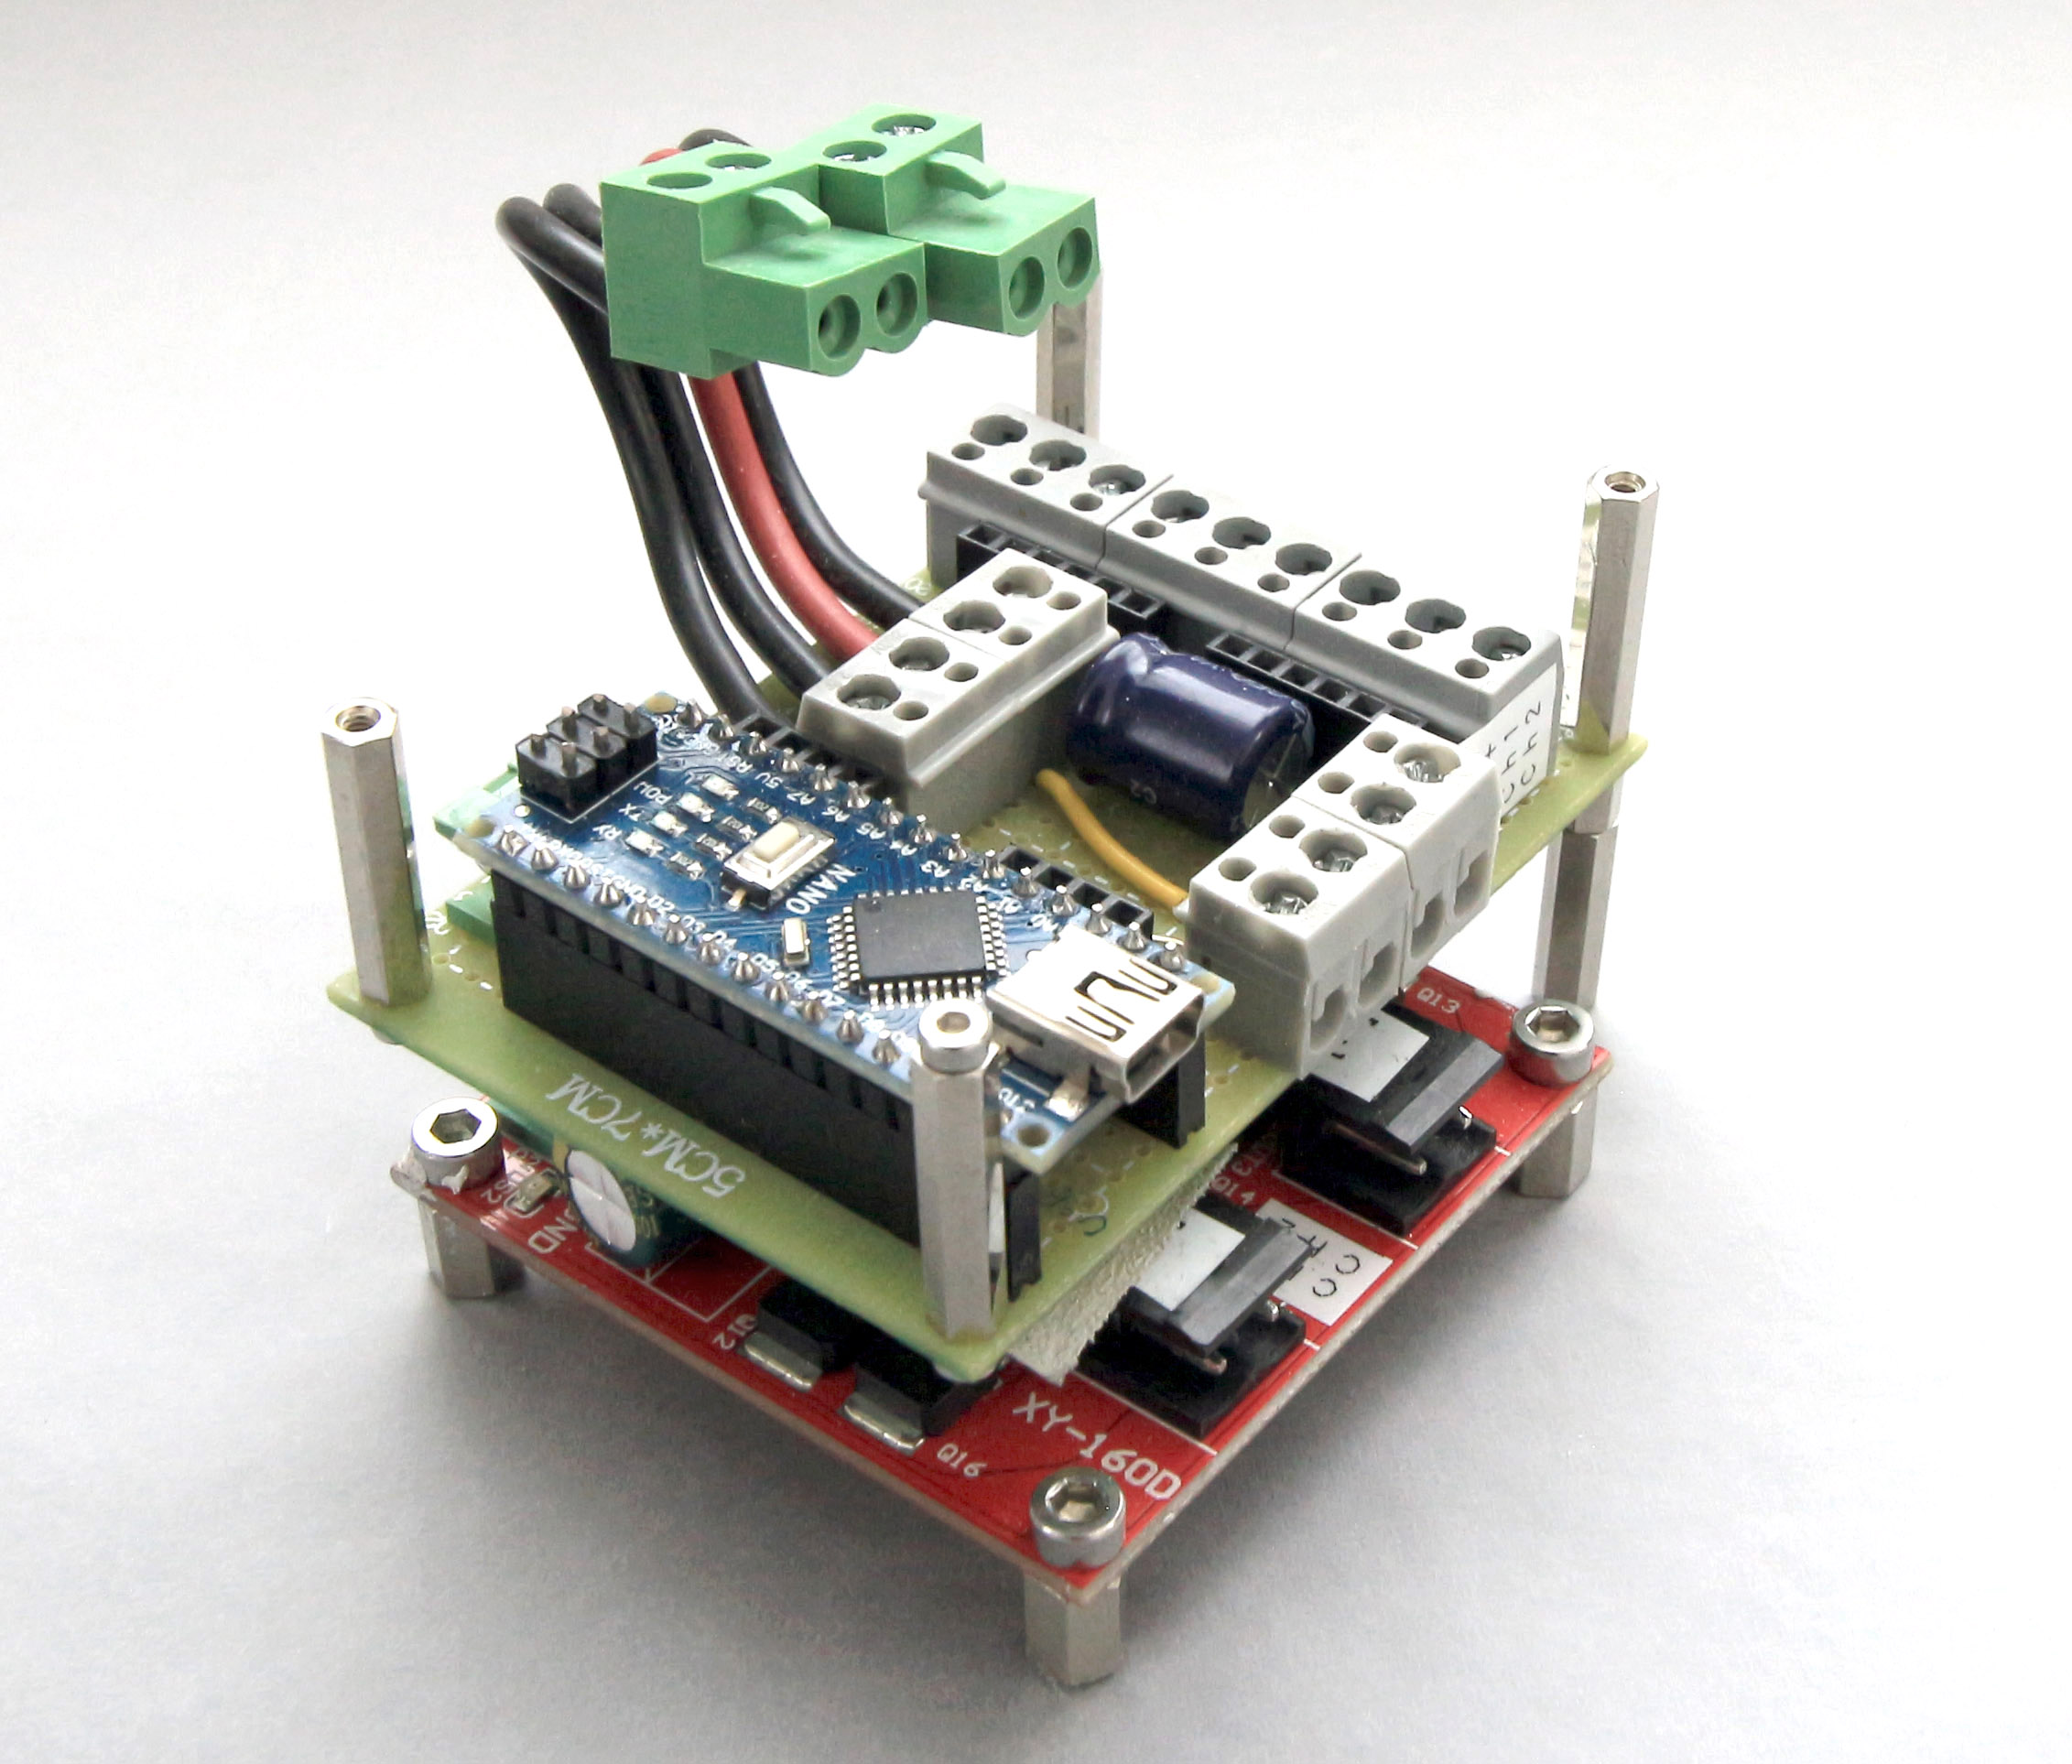
\includegraphics[width=0.90\textwidth]{images/04-3/controller-Photo-NoRadio.jpg}
    \caption{Photo of the CL1 Clamp Controller}
    \label{fig:photo-cl1-controller}
\end{figure}

\FloatBarrier

\subsection{CL1 Clamp Firmware}
\label{subsection:exploration-1-cl1-firmware}

The CL1 Clamp Firmware is an Arduino-based motor controller system written in C++ that can control two linear actuators and accepts serial communication for command and control. The main control loop implements non-preemptive scheduling for sharing time between three subroutines. All three subroutines are visited sequentially in each cycle and are allowed to run until it yields control (see Figure \ref{fig:firmware-motion-control-timeshare}). If needed, each subroutine can implement its own timer to determine how frequently it should be executed.\footnote{This feature was used only in later development when there are more subroutines.}.

\begin{enumerate}
    \item \textbf{Read and Process Serial Command} \\ Process command received from USB serial interface. This is intended for debugging as the controller was not yet integrated with wireless communication. \seeref{subsubsection:exploration-1-control-commands}
    \item \textbf{Motor Motion Control} \\ Only active when there is an active motion target. A separate timer is used to fix the motion control frequency. \seeref{subsubsection:exploration-1-bang-bang-motion-control}
    \item \textbf{Battery Monitor}\\ Check battery level using integrated ADC in microcontroller. \seeref{subsubsection:exploration-1-microcontroller}
\end{enumerate}

\begin{figure}[h]
    \centering
    \vskip 20pt
    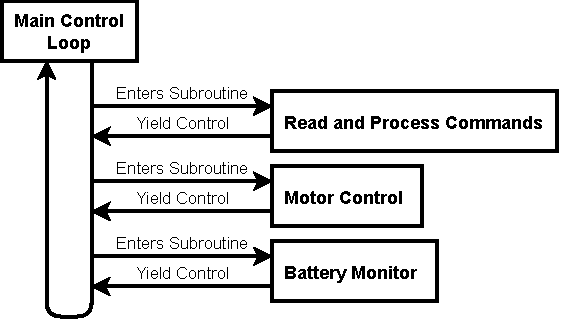
\includegraphics[width=0.60\textwidth]{images/04-3/cl1-firmware-mainloop.pdf}
    \caption{Diagram showing time sharing between subroutines in the main control}
    \label{fig:firmware-motion-control-timeshare}
\end{figure}

\FloatBarrier

\subsubsection{Control Commands}
\label{subsubsection:exploration-1-control-commands}

The CL1 Clamp Firmware was designed to receive serial commands from the integrated USB serial adapter and provide responses when necessary. Since the USB messaging protocol is completely transparent to the Arduino microcontroller, the serial interface is purely a stream of bytes transmitting at 115200 baud. Command messages are terminated by a '\textbackslash n' character and without start-of-message header. The Command Processing Subroutine monitors the receive buffer and triggers a response when a command is received.

\begin{table}[thb]
    \includegraphics[page=8, trim=25.4mm 130mm 25.4mm 33mm, clip, width=\textwidth]{tables/Tables in Chapter 4.pdf}
    \caption{Commands supported by the CL1 Clamp Firmware}
    \label{table:command-list-cl1-firmware}
\end{table}


All commands received by the firmware are treated as real-time commands, allowing motion to be started, modified, or stopped at any time. This is crucial for upper-level controllers (on a PC) to assert full control over the hardware behaviour and stop it in emergency situations. This behaviour is inspired by many embedded real-time Computer Numeric Control (CNC) motion controllers, such as tinyg2 \parencite{G2core2023} and grbl \parencite{jeonGrbl2019}. 
Table \ref{table:command-list-cl1-firmware} lists all the commands supported by the controller.


In order to avoid blocking the main control loop, all motion commands are processed in an asynchronous manner. This was achieved by setting an internal state in the controller, such as a target position, and defer the execution to the motion control subroutine in the main control loop. The Motion Control Subroutine can then be executed regularly to perform motion control \seeref{section:exploration-1-demonstration}. For other commands, such as the settings \verb|(\$)| commands, the status report \verb|(?)| and the stop command, were executed immediately. 

In this exploration round, there was no mechanism to ensure command packages are not lost during transmission. There was a risk that a movement command may be lost and the controller will not start the motion. This was a known issue that was addressed in the next exploration round \seeref{subsection:exploration-2-clamp-controller-l2}.

\FloatBarrier

\subsubsection{Bang Bang Motion Control}
\label{subsubsection:exploration-1-bang-bang-motion-control}



A linear profile motion controller was implemented to control the motion of the two motors based on encoder readings \parencite{tanPrecisionMotionControl2001}. The motion profile is defined by the following parameters:

\begin{itemize} [nosep]
    \item Velocity - Extracted from \verb|\$0| setting
    \item Start position - Current motor position when the motion command is received
    \item Target position - Target value defined in the motion command
    \item Start time - The time when the motion command is received
\end{itemize}

\begin{figure}[h]
    \centering
    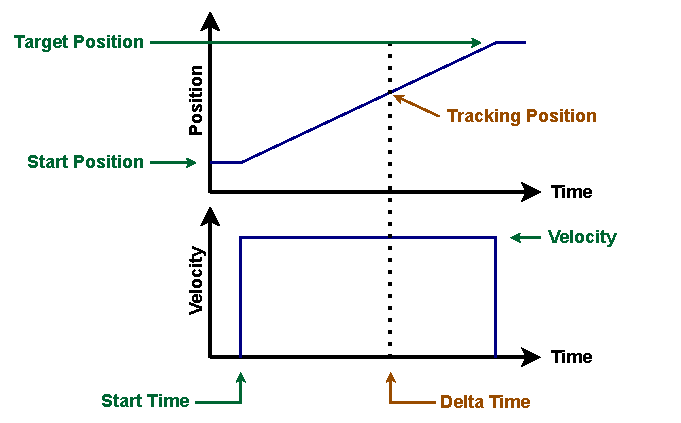
\includegraphics[width=0.99\textwidth]{images/04-3/firmware-motion-control.pdf}
    \caption{Linear motion profile of the CL1 Clamp Firmware}
    \label{fig:linear-motion-profile}
\end{figure}

When the Motor Control Subroutine is entered, it computes the current tracking position using the motion trajectory and computes the {\tt tracking\_position\_error} by comparing it with the encoder readings. 
Figure \ref{fig:linear-motion-profile} shows the motion profile in a graphical way. Green arrows are the parameters that define the motion profile and brown arrows are the changing tracking targets.
The equations of motion are as follows:

\begin{align*}
    delta\_time &= current\_time - motion\_starting\_time \nonumber \\
tracking\_position &= delta\_time \times velocity +  starting\_position \nonumber \\
tracking\_position\_error &= tracking\_position - current\_position \nonumber \\
\end{align*}

A bang-bang control logic is implemented for simplicity. When the position error is positive, the motor is set at full power to catch-up. Otherwise, the motor is set to cruising mode (no power, high impedance) and allowed to slow down. No control deadband was programmed. This low level control subroutine is not being throttled by a timer. Therefore it runs as frequently as the main control loop and therefore it may be executed irregularly. Despite the simplicity of bang-bang control, it was tested to be functional over a variety of speed from 0 to 2mm/s. The mechanical dampening likely contributed to its relatively smooth motion.

During the motion tracking, if the position error is too large, the controller will consider it as a tracking failure and will switch over to a stopped state. This is a protection for when the assembly resistance is too great for the motor to keep up with the designated speed. It is possible to try a failed motion again with a slower speed, but tests have shown that the assembly resistance will eventually increase to the point that the motor cannot keep up again. In general this is referred to as a stall state. 

Extra protection was added to avoid overheating the motor and the driver. This is implemented by detecting whether the encoder values have changed within a certain time. If power was applied to the motor and the encoder did not rotate, the controller would stop and enter the stalled state. 

Table \ref{table:cl1-firmware-motion-control-parameters} shows the main control parameters and their tuned values used in the demonstration. The motion control algorithm is validated with the CL1 hardware and its positioning repeatability is within 0.2mm.

\begin{table}[h]
    \includegraphics[page=9, trim=25.4mm 220mm 25.4mm 33mm, clip, width=\textwidth]{tables/Tables in Chapter 4.pdf}
    \caption{Motion control parameters of the CL1 Clamp Firmware}
    \label{table:cl1-firmware-motion-control-parameters}
\end{table}

\FloatBarrier

\section{Demonstration}
\label{section:exploration-1-demonstration}

\subsection{Design considerations}
\label{subsection:exploration-1-design-considerations}

Figure \ref{fig:timber-joint-for-cl1-test} shows the timber joint used for validating the clamping movement. The column and the beam have a 100mm x 100mm profile size. The half-lap joints are orthogonal, each being 50mm thick. The joints were cut manually with a pull saw very carefully. Four 10mm x 10mm registration holes for the hanging gripper were drilled using the drill guide shown in \noseeref{subsubsection:exploration-1-gripper-for-hanging-clamp}. Figure \ref{fig:timber-joint-for-cl1-test-ground-support} shows the vertical column mounted on a rigid base on the ground in preparation of the clamping motion test.



It requires approximately 0.9kN force to be assembled, confirmed using a setup similar to the test conducted in \noseeref{subsection:exploration-1-joint-tightness} but oriented horizontally.

\subsection{Execution Preparation}
\label{subsection:exploration-1-execution-plan}

The list below shows a number of planned tests with the CL1 Clamp. They were successfully executed until the Clamp Stall Test, which damaged the clamp. Nevertheless, the lessons learnt from this clamp design and construction experience is sufficient to move on to the next exploration round. Therefore the damaged clamp was not repaired to continue the rest of the planned tests.

\begin{figure}
    \centering
    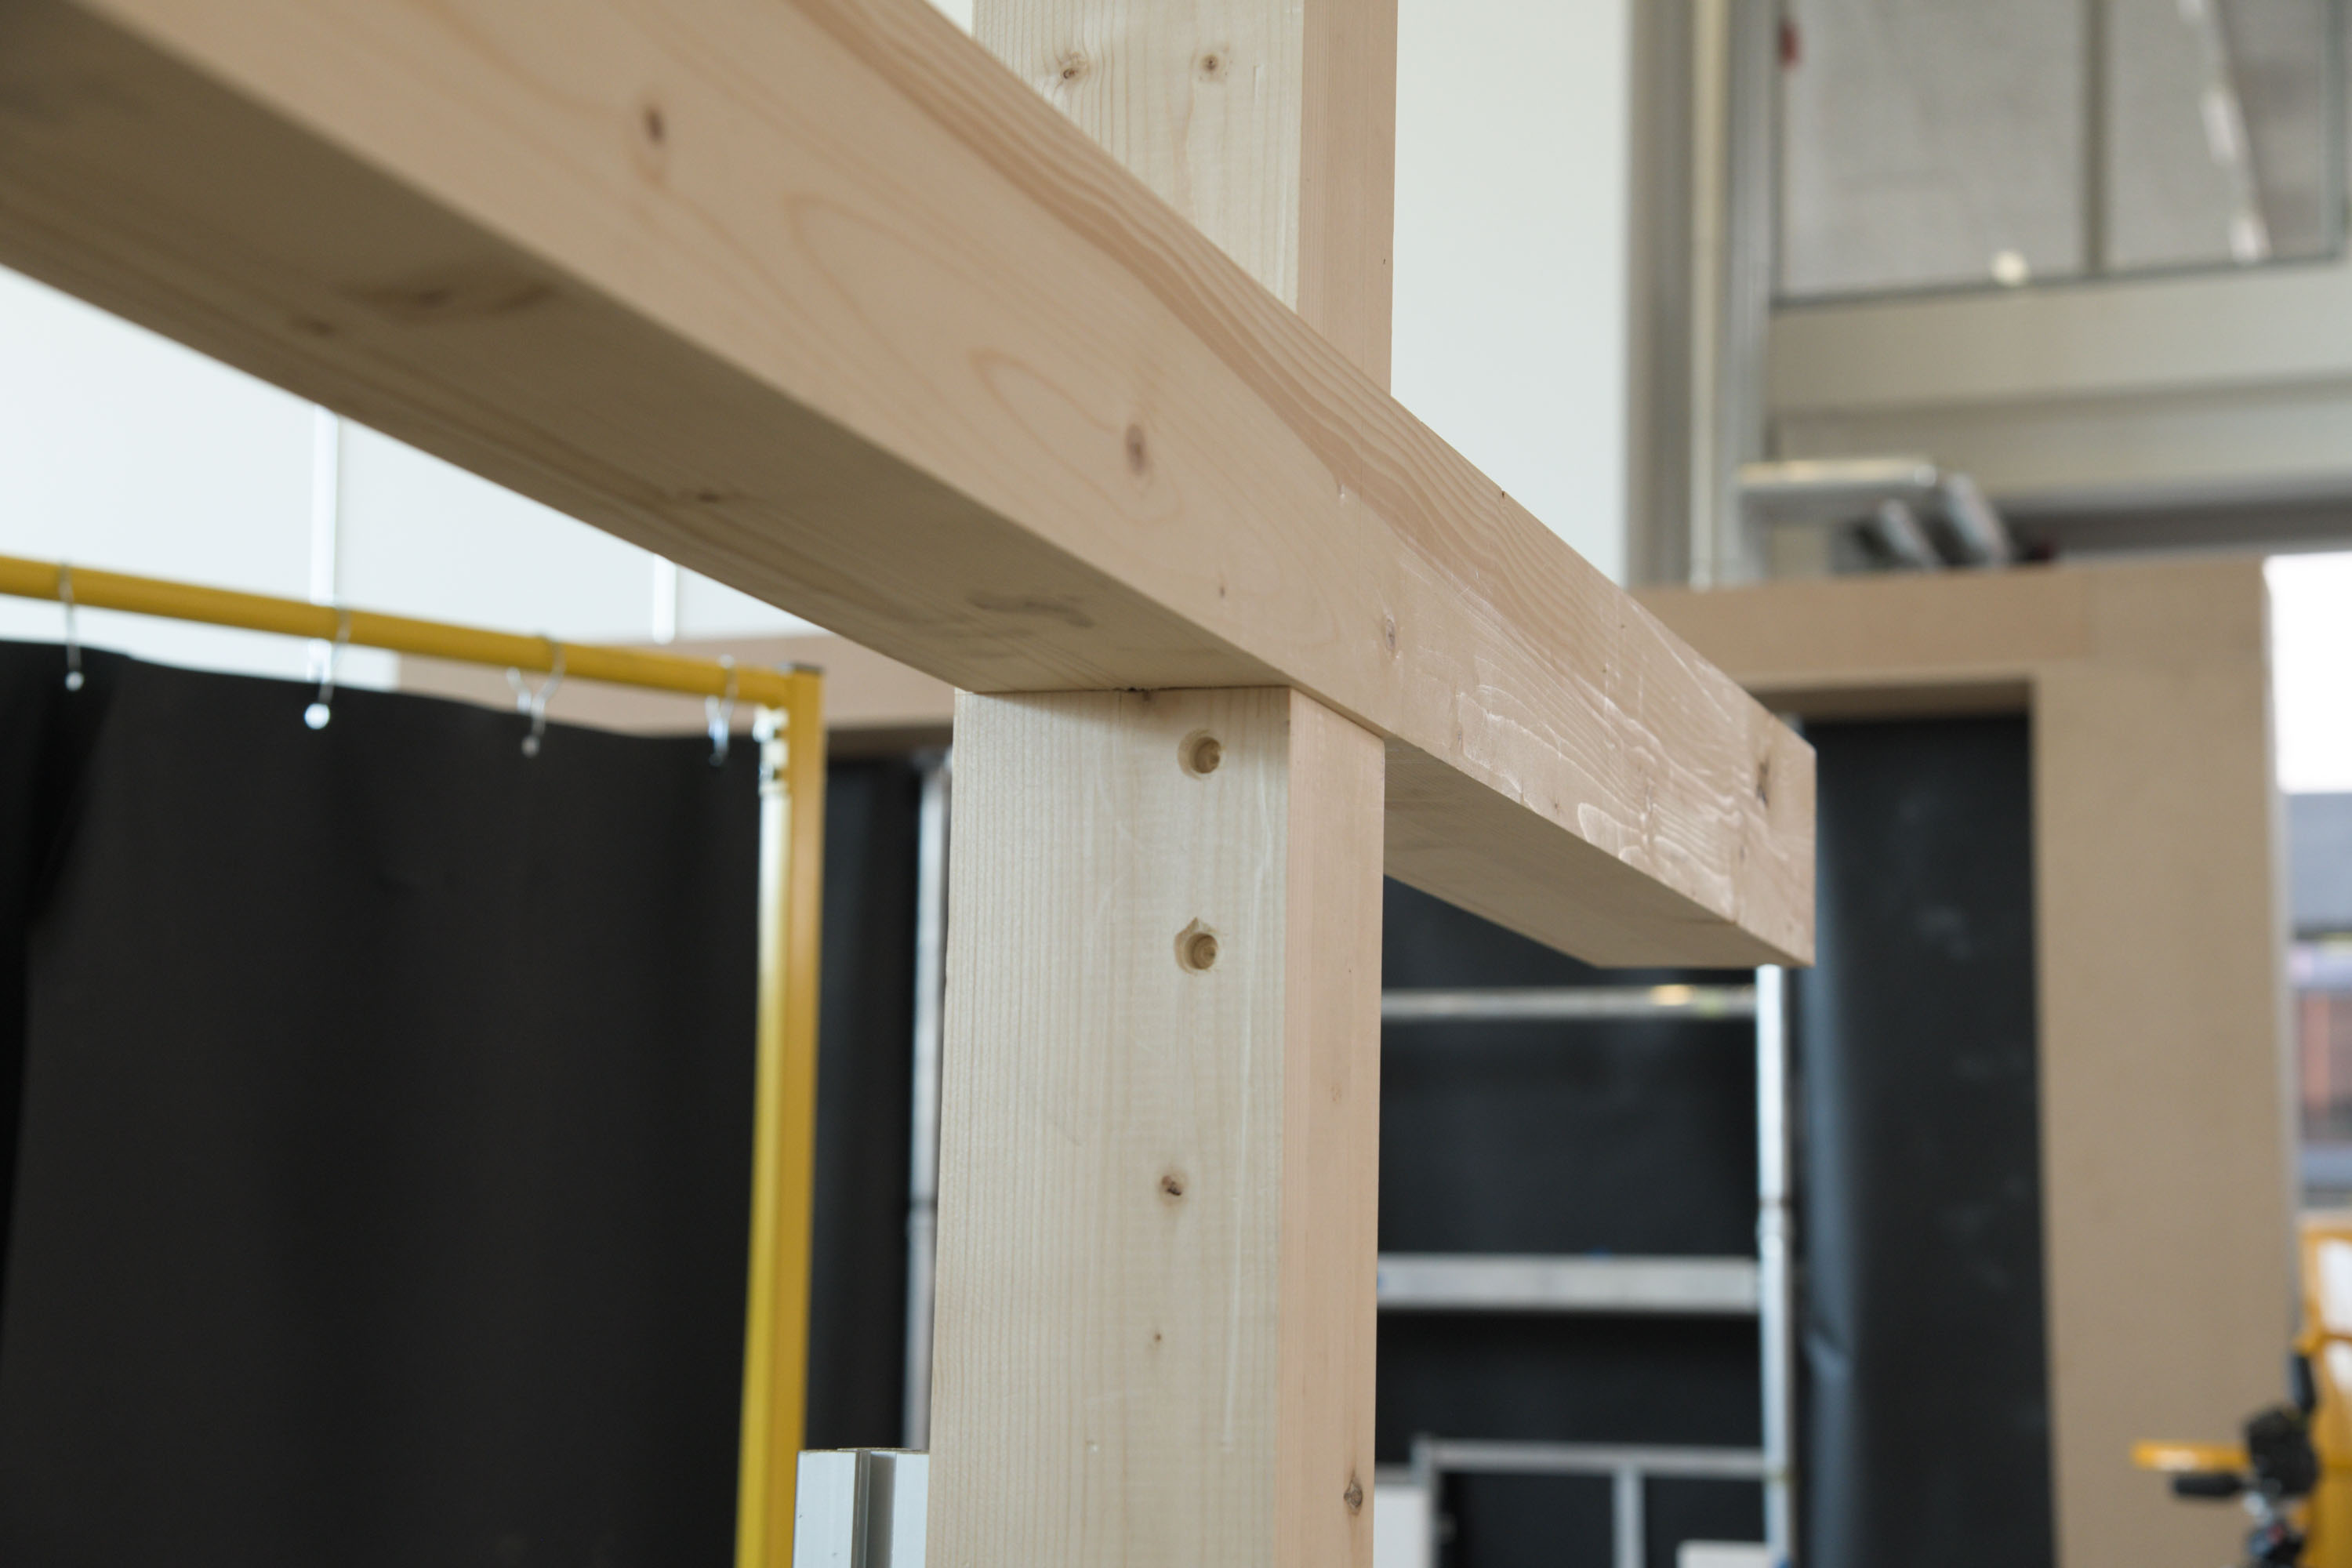
\includegraphics[width=0.99\textwidth]{images/04-4+5/cl1-test-wood.jpg}
    \caption{Timber joint used for validating the clamping movement}
    \label{fig:timber-joint-for-cl1-test}
\end{figure}


\begin{samepage}
\begin{itemize}
    \item Construct column setup
    \begin{itemize}[nosep]
        \item Vertically column rigidly fixed to ground (see Figure \ref{fig:timber-joint-for-cl1-test-ground-support})
        \item Manually attach clamp to column
    \end{itemize}
    \item Clamping Motion Test (repeated 4 times)
    \begin{itemize}[nosep]
        \item Clamp jaw set to fully extended (105mm position)
        \item Manually place horizontal beam into clamp jaw (see Figure \ref{fig:manual-place-beam})
        \item Clamp jaw set to move towards clamped position (0mm), automatically start closing at 2mm/s. (see Figure \ref{fig:cl1-clamp-closing-photo})
    \end{itemize}
    \item Clamp Stall Test (tested to failure, see \noseeref{subsection:exploration-1-damaged-actuator-gearbox})
    \item Clamping Speed Test (cannot be performed)
    \item Load Cell Data Collection (cannot be performed)
    \item Clamping in Different Orientations (cannot be performed)
\end{itemize}
\end{samepage}

\begin{figure}
    \centering
    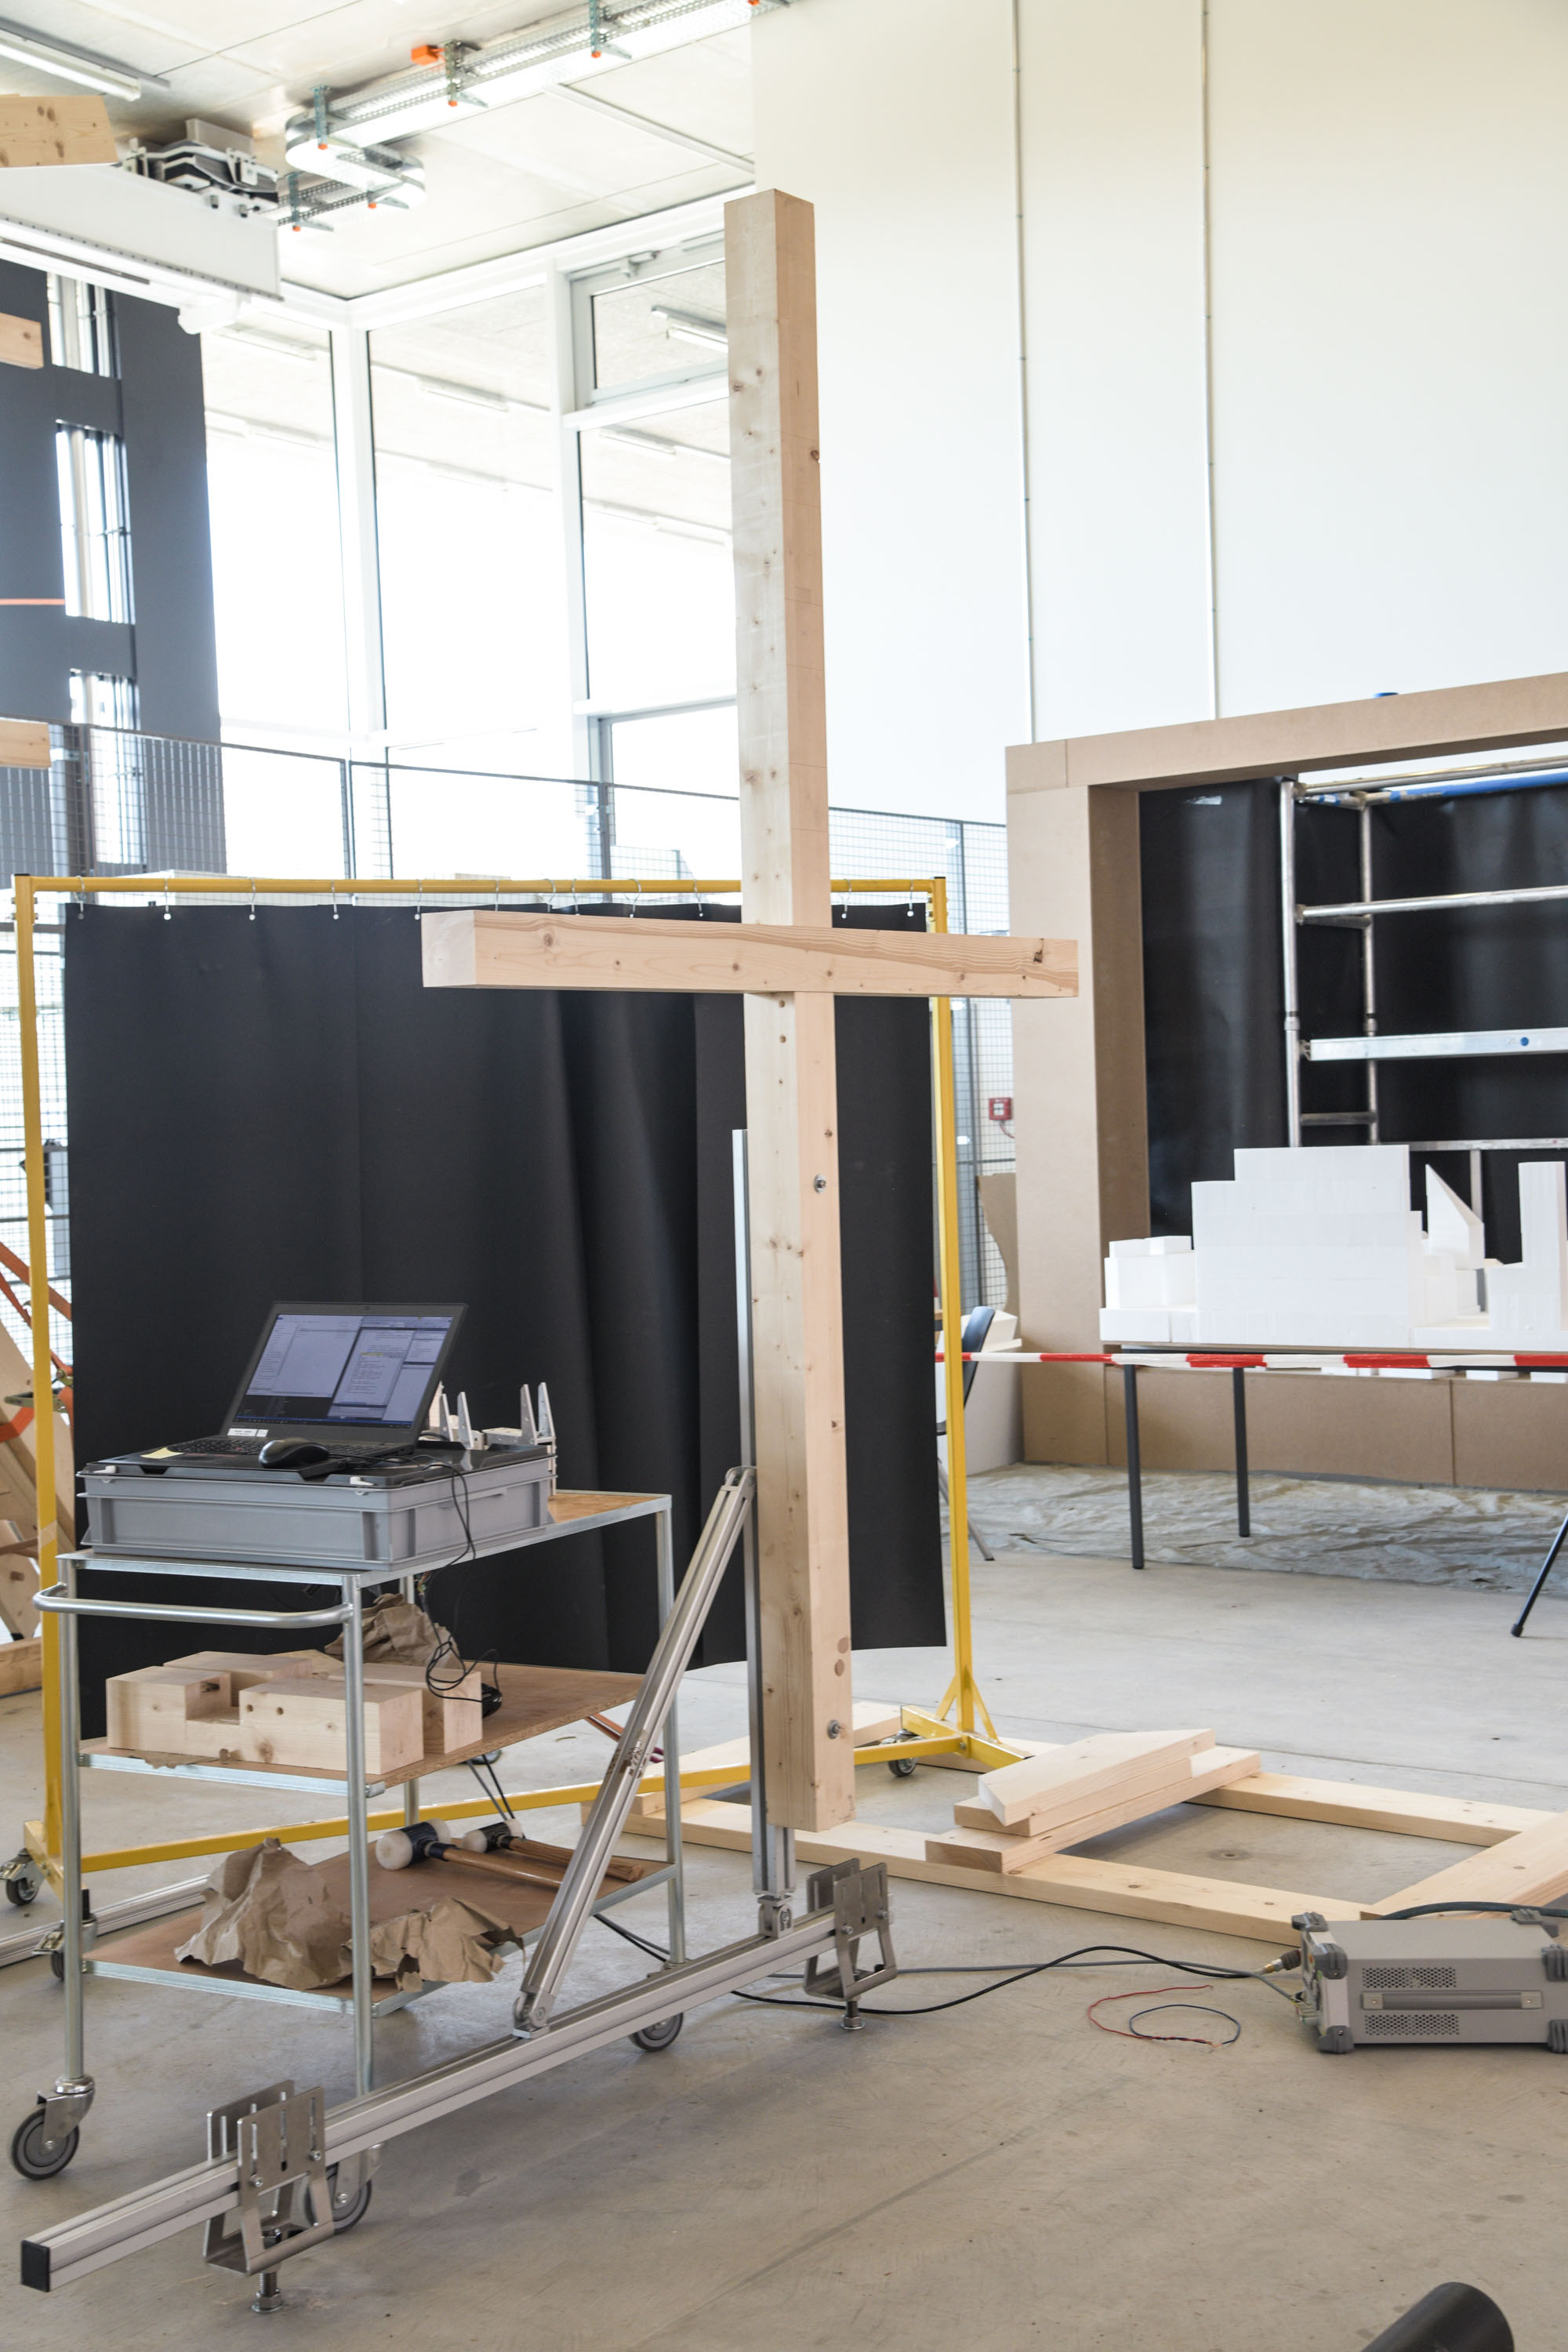
\includegraphics[width=0.99\textwidth]{images/04-4+5/cl1-test-wood-mount.jpg}
    \caption{Rigid support for the column during clamping motion test}
    \label{fig:timber-joint-for-cl1-test-ground-support}
\end{figure}

\FloatBarrier

\section{Lessons Learnt}
\label{section:exploration-1-lessions-learnt}

\subsection{Successful Validation}
\label{subsection:exploration-1-successful-validation}

During the setup, a manual valve was used to actuate the hanging gripper and there was no difficulty positioning the clamp on the column. Figure \ref{fig:cl1-clamp-hanging-photo} shows the clamp hanging from the column. The spring loaded grip between them was firm and stable. 

\begin{figure}[h]
    \centering
    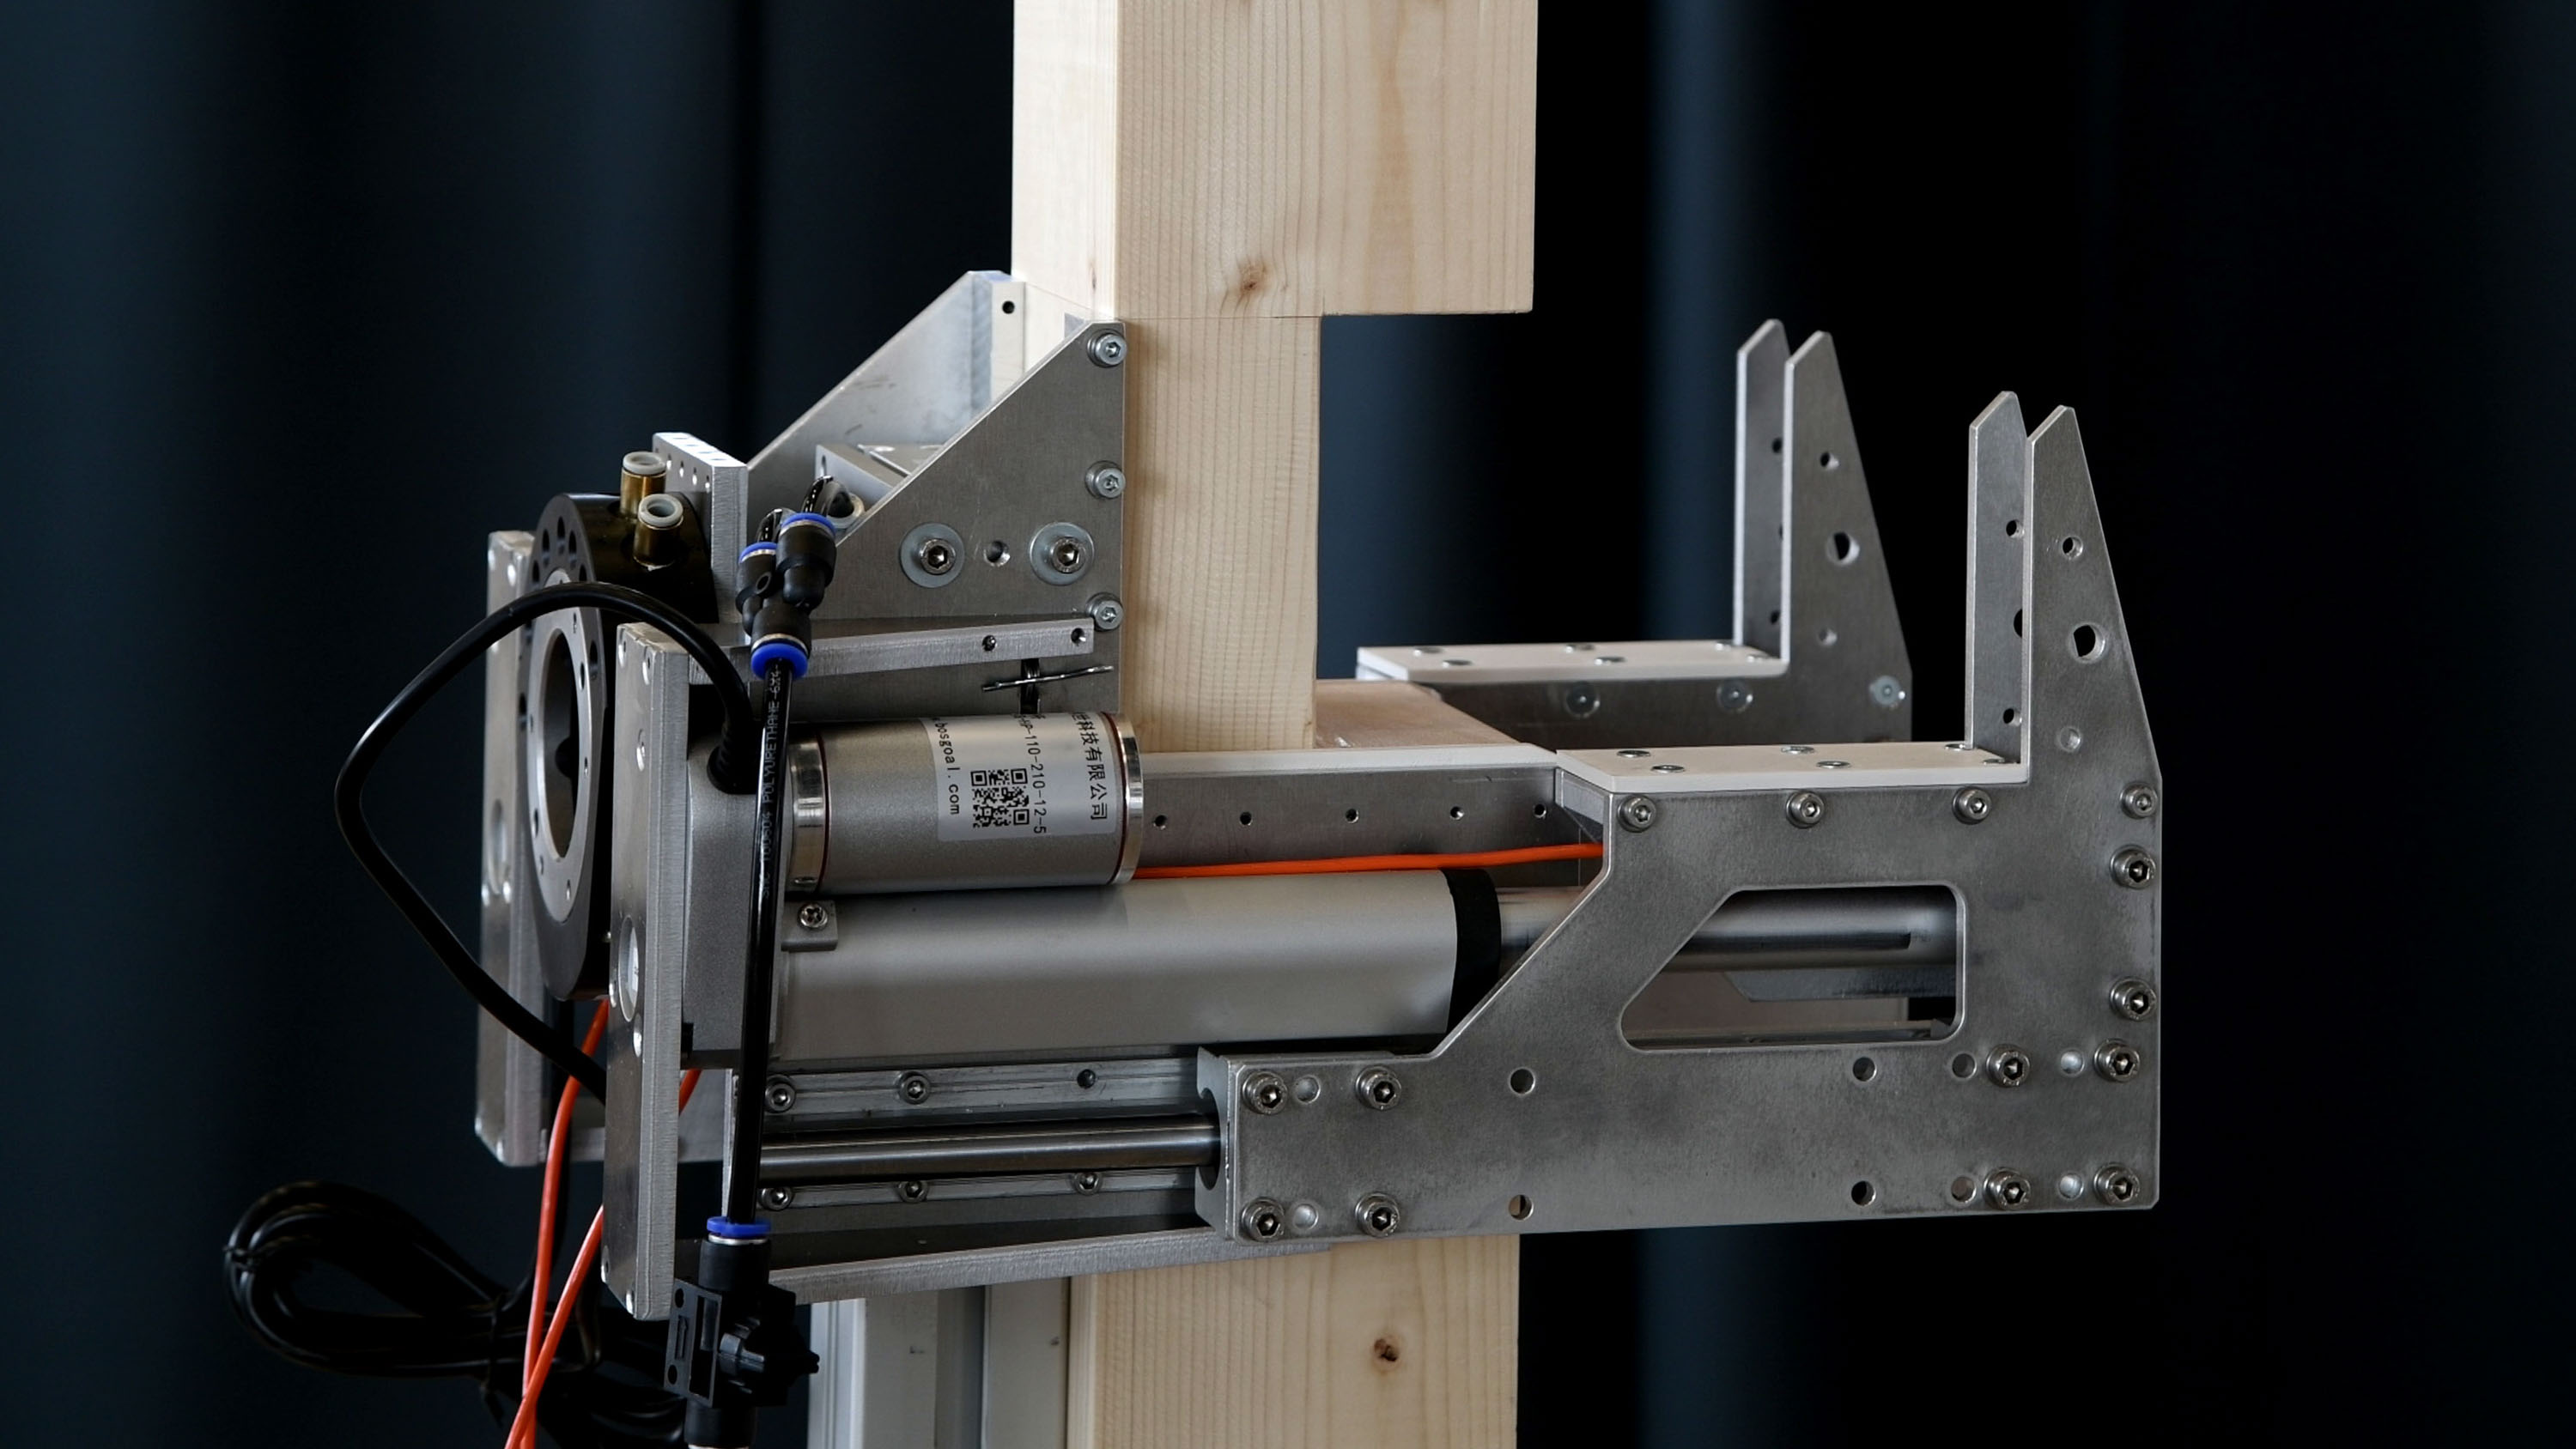
\includegraphics[width=0.99\textwidth]{images/04-4+5/cl1-test-closeup.jpg}
    \caption{CL1 clamp hanging from the column}
    \label{fig:cl1-clamp-hanging-photo}
\end{figure}

The clamp’s weight is 4.9kg without a battery. This raised a concern for its future when it is not hanging in a perfectly vertical column because this much mass may cause a lot of deformation to the partially-assembled structure. Nothing was done to address this problem in this Exploration Round because it did not cause a problem for the test. In the next rounds, the weight issue was gone because of the new clamp designs. 

Figure \ref{fig:manual-place-beam} shows the manual placement of the beam into the clamp jaws. It was carefully placed to align the two halves of the lap joint. The horizontal surface in the clamp jaw was found capable of supporting the beam steadily. However, it was also apparent that this would not have been possible if the beam had been tilted at an angle \seeref{subsection:exploration-1-beam-support-needed-during-clamping}.

\begin{figure}
    \centering
    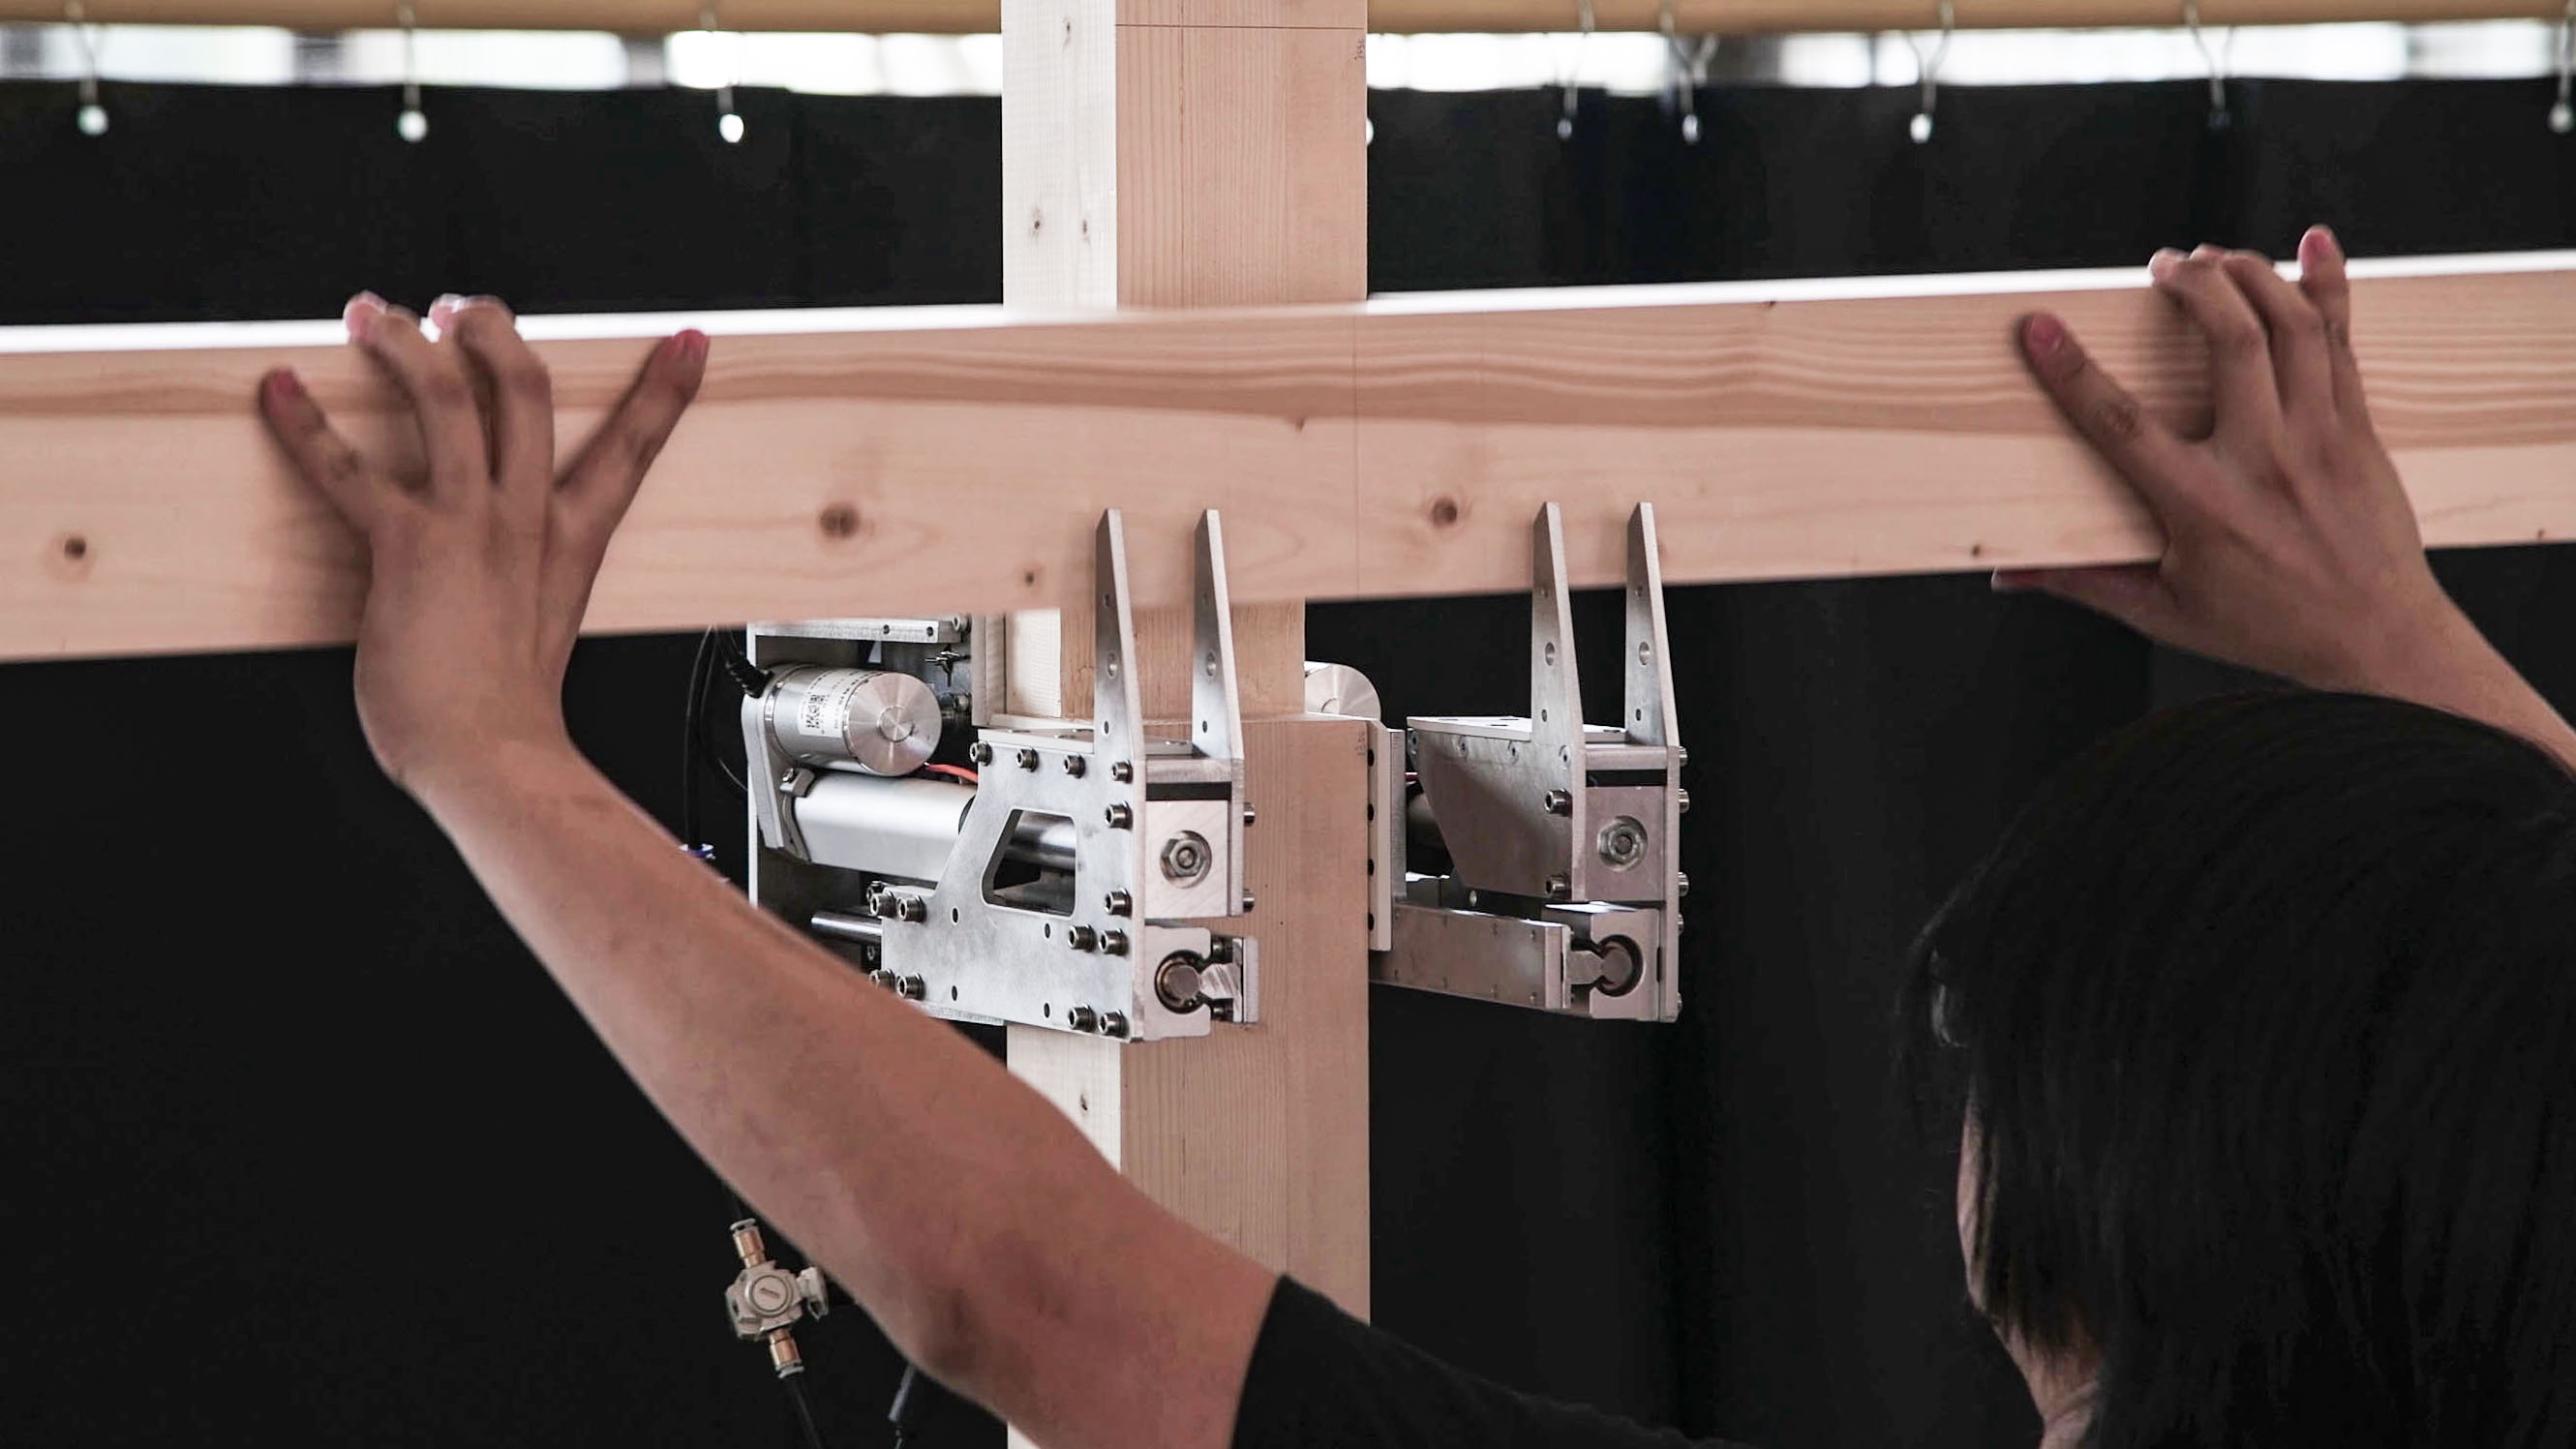
\includegraphics[width=0.99\textwidth]{images/04-4+5/experiment-manual-place-beam.jpg}
    \caption{Manually placing the beam into the clamp jaws}
    \label{fig:manual-place-beam}
\end{figure}

There was no alignment features used between the beam and the clamp jaw, as was intended in the initial design. The plan was to first test without the features before introducing them. However, the instability problem if the beam were to be tilted, makes this exploration obsolete as it is clear that a different alignment solution is needed.

During the robotic motion, both jaws maintained steady and synchronous movement at 2.5mm/s, the total distance travelled was 105mm (see Figure \ref{fig:cl1-clamp-closing-photo}). The horizontal beam can be seen moving steadily without slip-stick behaviour while closing the joint.  

\begin{figure}
    \centering
    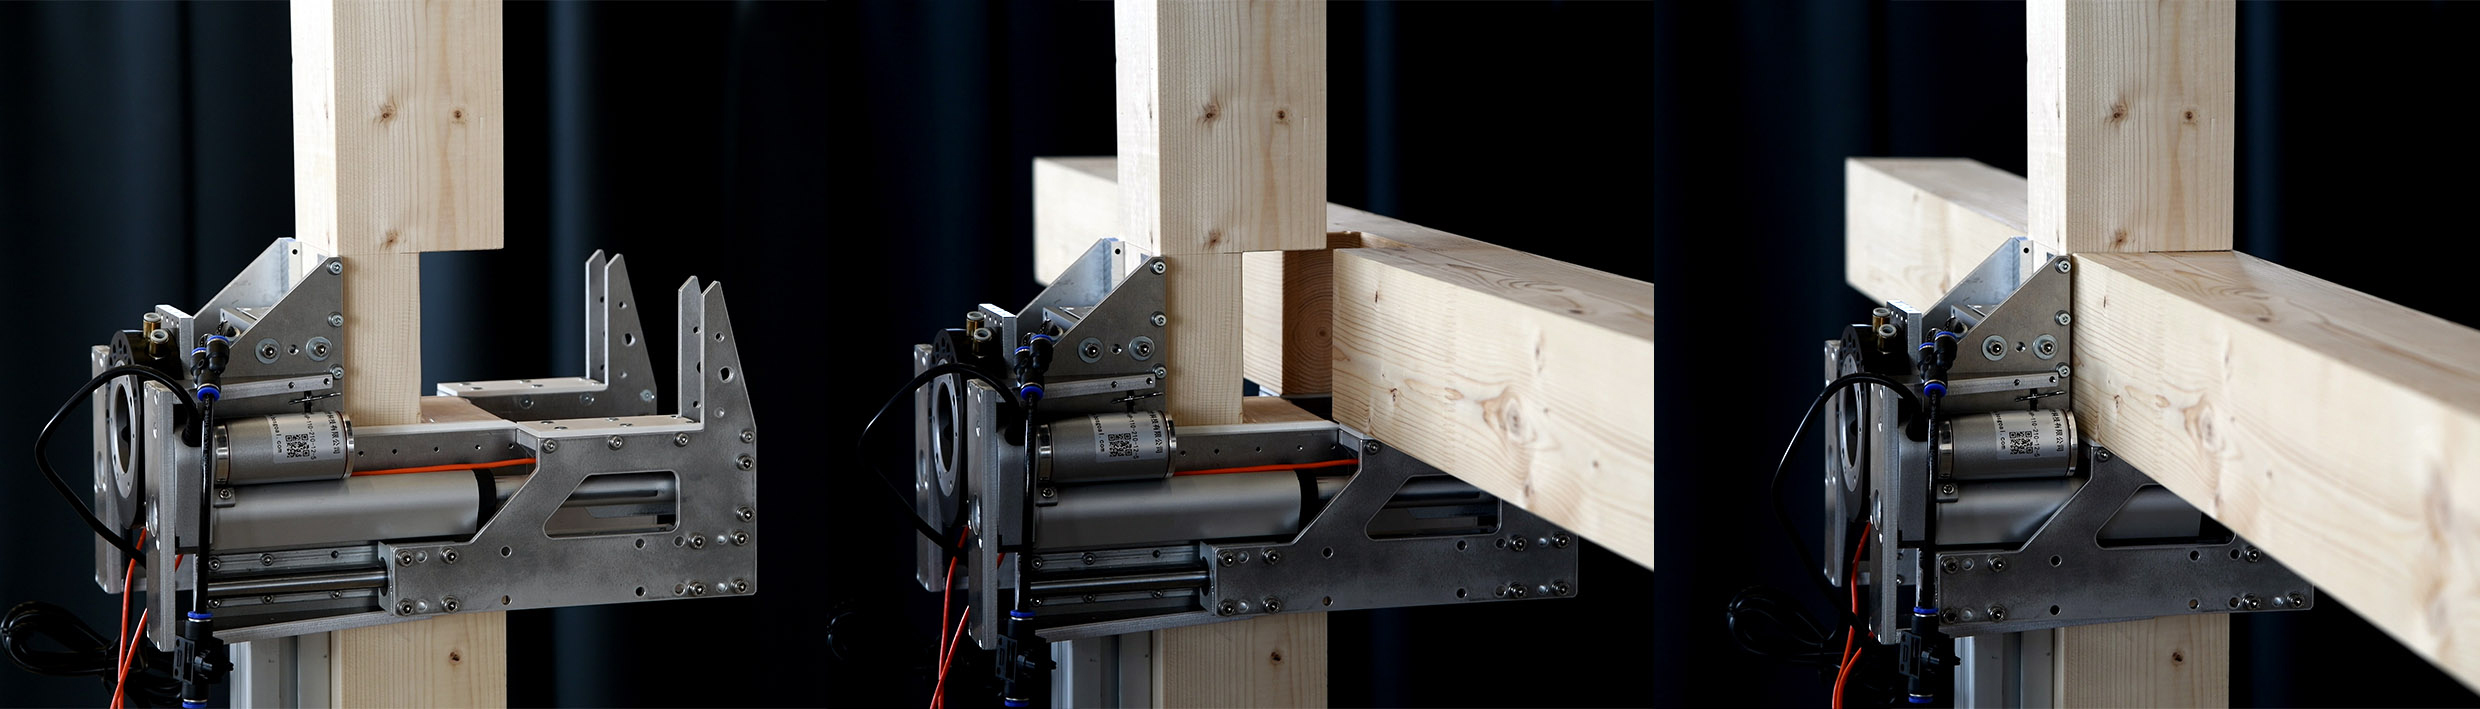
\includegraphics[width=0.99\textwidth]{images/04-4+5/cl1-test-threesteps.jpg}
    \caption{CL1 clamp closing on the beam}
    \label{fig:cl1-clamp-closing-photo}
\end{figure}

The following design features are validated:
\begin{itemize}
    \item The choice of the guided parallel gripper as the gripper body was rigid enough for hanging the clamp on the timber (other hanging orientation was also tested).
    \item The geometry of the hanging gripper registration features were capable of aligning the clamp to the pre-drilled holes on the beam.
    \item The choice of hanging gripper spring was sufficient to keep the clamp attached.
    \item The pre-drilled 10mm holes did not get damaged.
    \item The mechanical design of the clamp jaw can survive the clamping action.
    \item The servo control for the two motors to perform synchronous motion was successful.
\end{itemize}

\subsection{Damaged actuator gearbox}
\label{subsection:exploration-1-damaged-actuator-gearbox}

During the second test - Stall Test, a solid piece of timber was placed in the jaw to prevent the clamp from closing. This is to validate whether the mechanical parts can survive a full strength motor stall. The maximum power limit on the driver was set to 100\%.

The clamp jaw is able to close until 150mm before it touches on the solid piece of timber. A crack can be heard soon after contact as stress buildup and power was turned off. Inspection upon releasing shows that the gearbox of the linear actuator has cracked and separated from its mounting (see Figure \ref{fig:cl1-damaged-gearbox-photo}). This structural failure stopped the test schedule and the subsequent tests were not performed.

\begin{figure}[h]
    \centering
    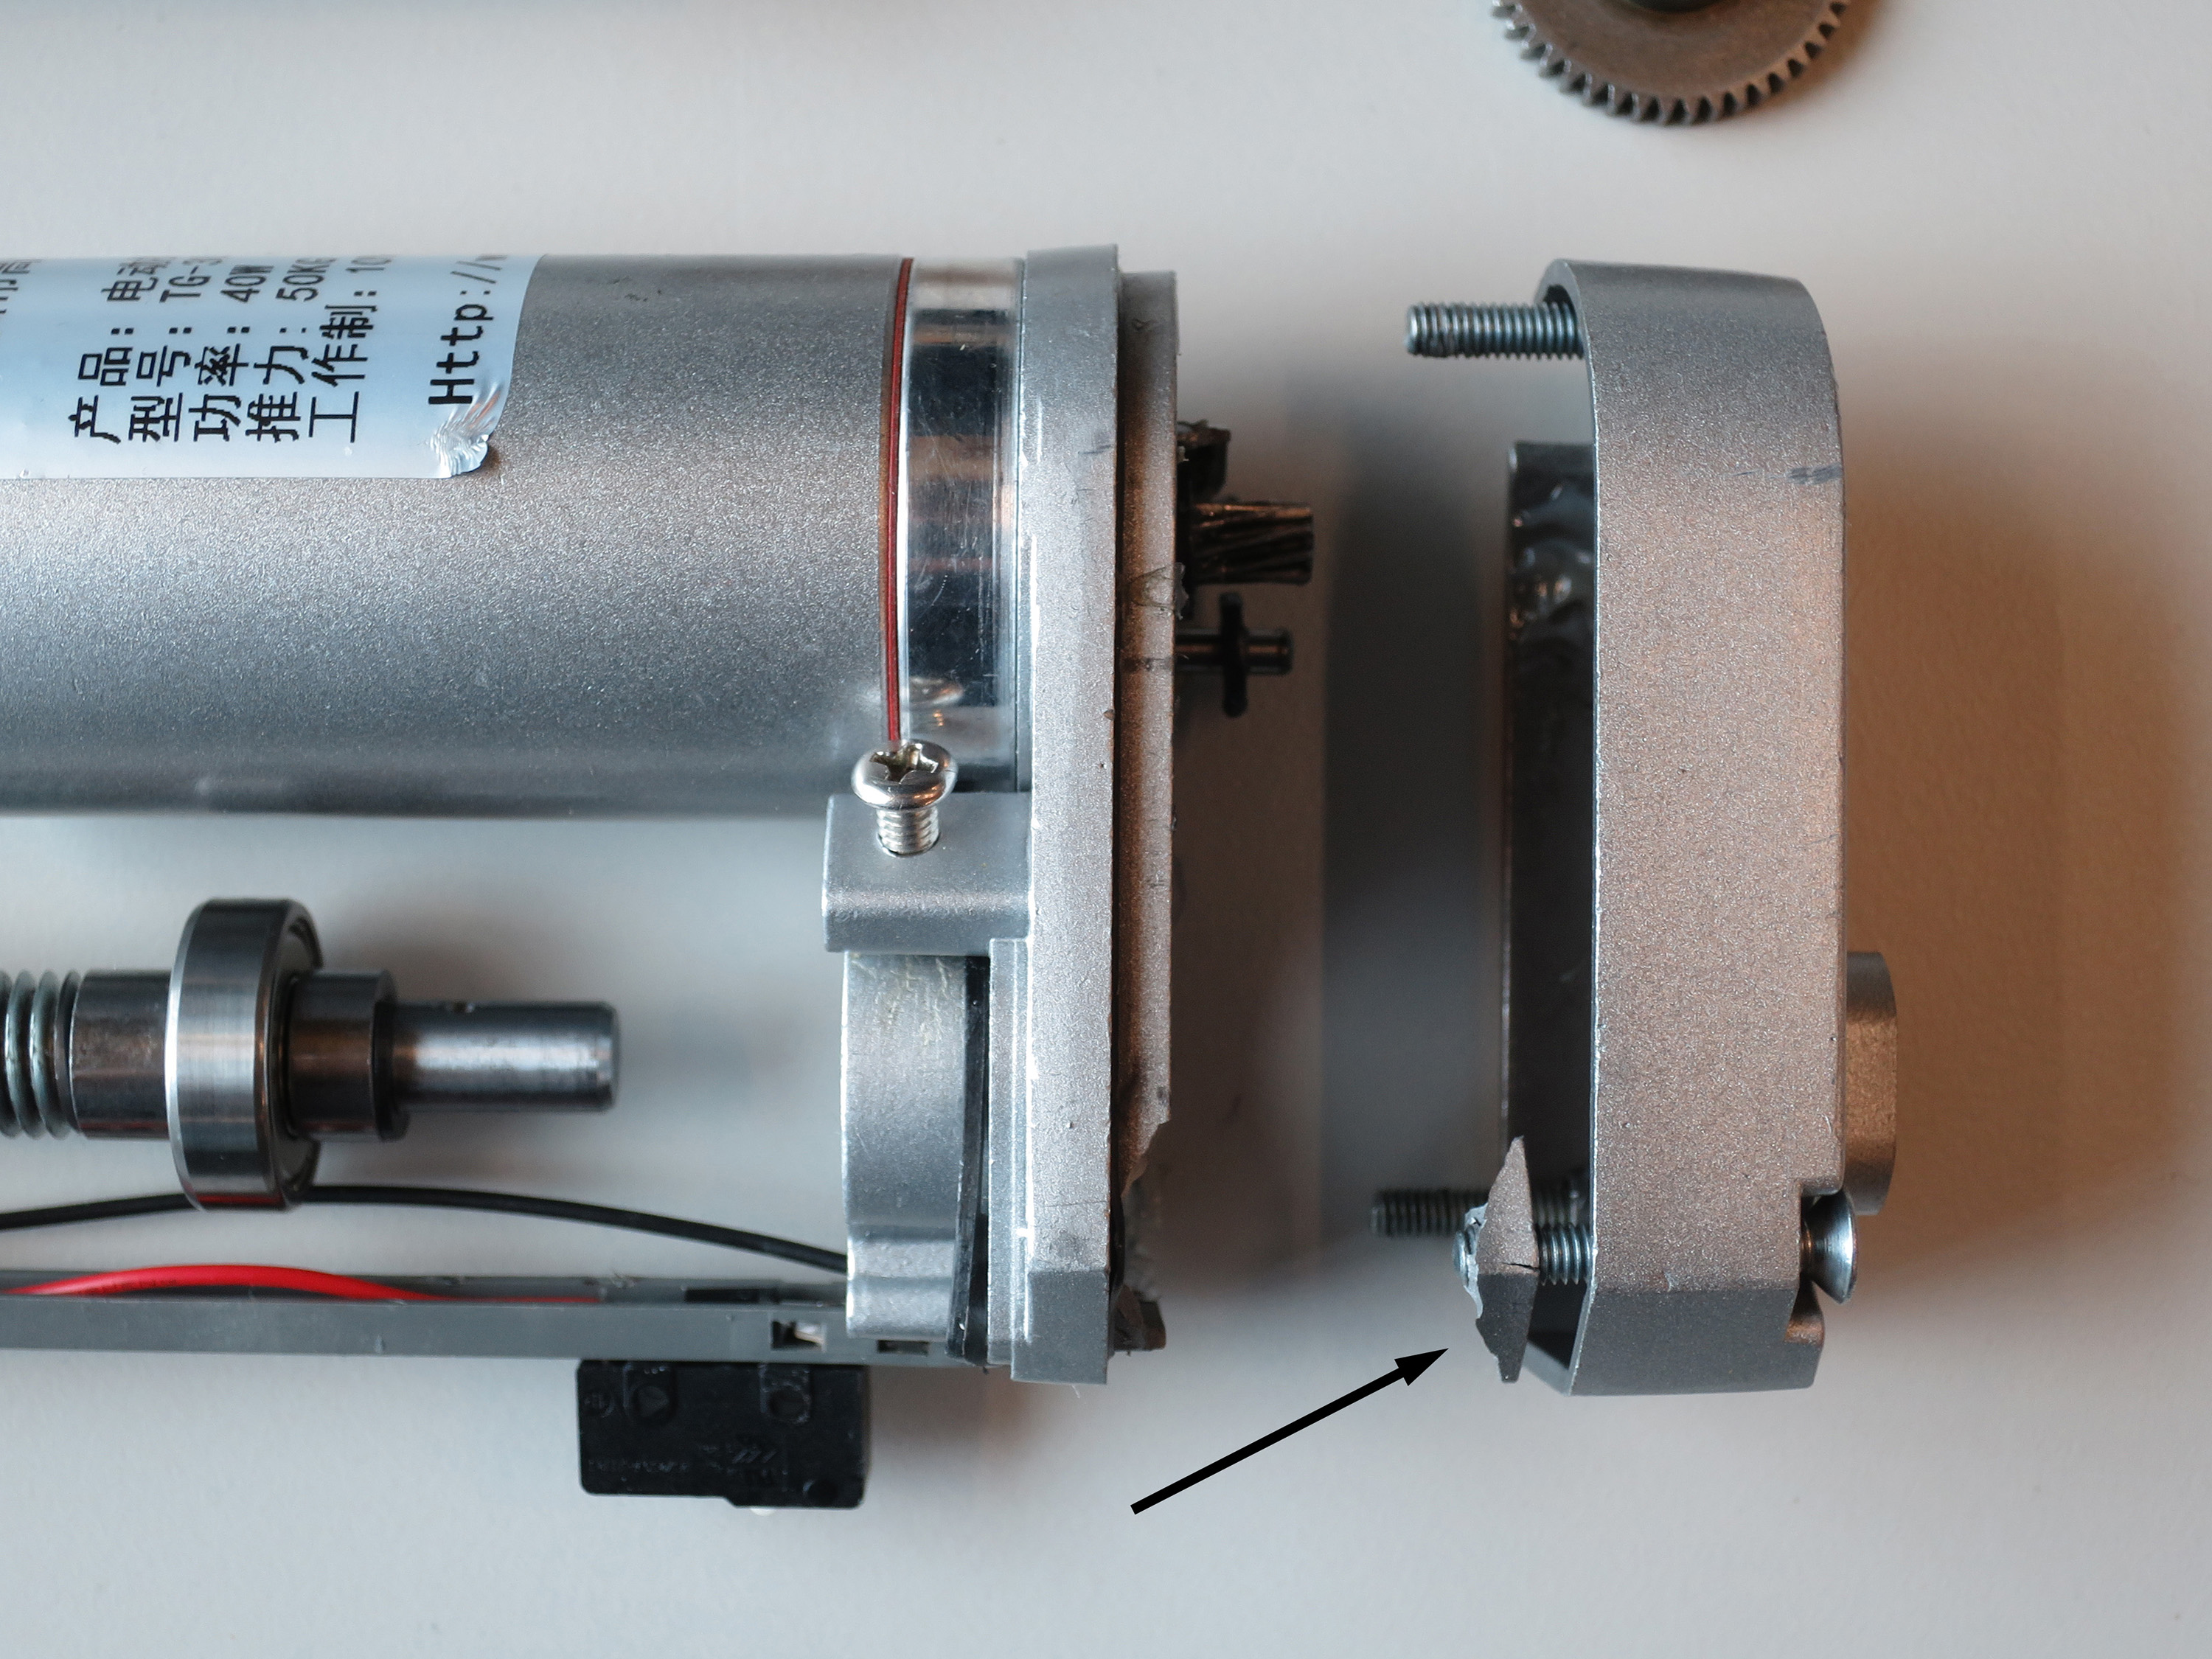
\includegraphics[width=0.99\textwidth]{images/04-4+5/cl1-damaged-gearbox-witharrow.jpg}
    \caption{Damaged gearbox of the linear actuator, with arrow pointing to the crack}
    \label{fig:cl1-damaged-gearbox-photo}
\end{figure}

\paragraph{Possible Cause}

\begin{itemize}[nosep]
    \item Despite not being specified by the manufacturer, the linear actuator is likely designed to be used for pushing against a compressive load. The use case here required the actuator to pull, and thus, its body is subjected to tension. 
    \item The mounting plate is connected to the casing of the gearbox that is not intended for this purpose.
\end{itemize}

\paragraph{Possible Solution and Follow-Up}

A quick search revealed that off-the-shelf linear actuators capable of pulling a few kN of tension are physically too big for the clamp. Possible solutions include:

\begin{itemize}[nosep]
    \item Commission a custom linear actuator from a fabricator
    \begin{itemize}
        \item This is not pursued because of budget concerns.
    \end{itemize}
    \item Design and build a custom screw mechanism for linear actuation
    \begin{itemize}
        \item Implemented and tested with success in the next Exploration Round \seeref{subsection:exploration-2-ball-screw-linear-actuator}. 
    \end{itemize}
\end{itemize}

Upon reflection, it is likely that if the motor were stalled long enough, the motor driver would also overheat and become damaged. The solution would require the firmware to include stall detection and cut power to the driver if a stall is detected. This is implemented when designing the next motion control algorithm \seeref{subsection:exploration-2-motion-control-for-dc-servo-motor}
This reflection also led to the realisation of a new protection concept for all DiRT tools: 
\begin{quote}
    The design of any DiRT tool should protect against self-destruction. The actions of the DiRT tool, even under incorrect control, should never cause irreversible damage to its own components.
\end{quote} 
This concept remained relevant for the rest of the thesis guiding the mechatronics development of later tools and systems.

\subsection{Electronics Brownout}
\label{subsection:exploration-1-electronics-brownout}

The electronics brownout problem refers to the microcontroller resetting its program \seeref{subsection:exploration-1-cl1-firmware} during operation due to a drop in supply voltage. This happened on a few occasions during unit tests of the actuator.

\paragraph{Possible Cause}

In the schematic design, the battery power rail supplies unregulated power ($\sim$ 14.8V) to the motor driver. It also supplies regulated low-voltage power (5V) to the microcontroller through a linear regulator. When overcoming large assembly resistance, the motor driver is instructed by the microcontroller to draw a high current from the battery power rail to power the actuator motor. There is a chance that the voltage on this rail drops below the regulator’s input limit and causes the regulated 5V to fall. This can cause the microcontroller to reset itself.

In the linear regulator design, input and output capacitors were provided to buffer sudden current draw. However, there is no protection against the motor driver draining the input capacitor.

\paragraph{Possible Solution and Follow-Up}

\begin{itemize}[nosep]
    \item Add diode before regulator input capacitors - This should help prevent the motor driver from drawing power from the regulator capacitor. The capacitor placed before the regulator should provide sufficient buffering capacity for maintaining regulated voltage on the digital side during maximum motor output.
    \begin{itemize}
        \item This was implemented and tested in Exploration Round 2 \seeref{subsection:exploration-2-cl3-clamp-electronics}
    \end{itemize}
    \item Add digital stall protection in motor controller firmware to limit stall duration. 
    \begin{itemize}
        \item This was implemented and tested successfully in Exploration Round 2 \seeref{subsection:exploration-2-motion-control-for-dc-servo-motor}
    \end{itemize}
    \item Use a separate battery for microcontroller - This could be a very stable solution and can potentially be very robust. However, this also adds an extra battery on-board and would increase operator workload to replace and recharge. 
    \begin{itemize}
        \item This was not implemented because the other solutions were sufficient.
    \end{itemize}
\end{itemize}

\subsection{Unstable Clamp Jaw}
\label{subsection:exploration-1-unstable-clamp-jaw}

The unstable clamp jaw problem was discovered almost immediately after the CL1 design was constructed. It is caused by a design error of using round linear bushings and assuming the linear actuator can act as the second linear guide. 

Unfortunately, due to the mounting points provided by the actuator, it is difficult to fix its base rigidly to provide enough stiffness against rotation. The rotational motion of the jaw does not cause any operational problem during the tests. However, there is a chance that this movement creates unintentional forces to other components and causes damage. Figure \ref{fig:cl1-broken-jaw-photo} of CL1 with the disassembled jaw shows the two round bushings that contributed to the instability.

\begin{figure}
    \centering
    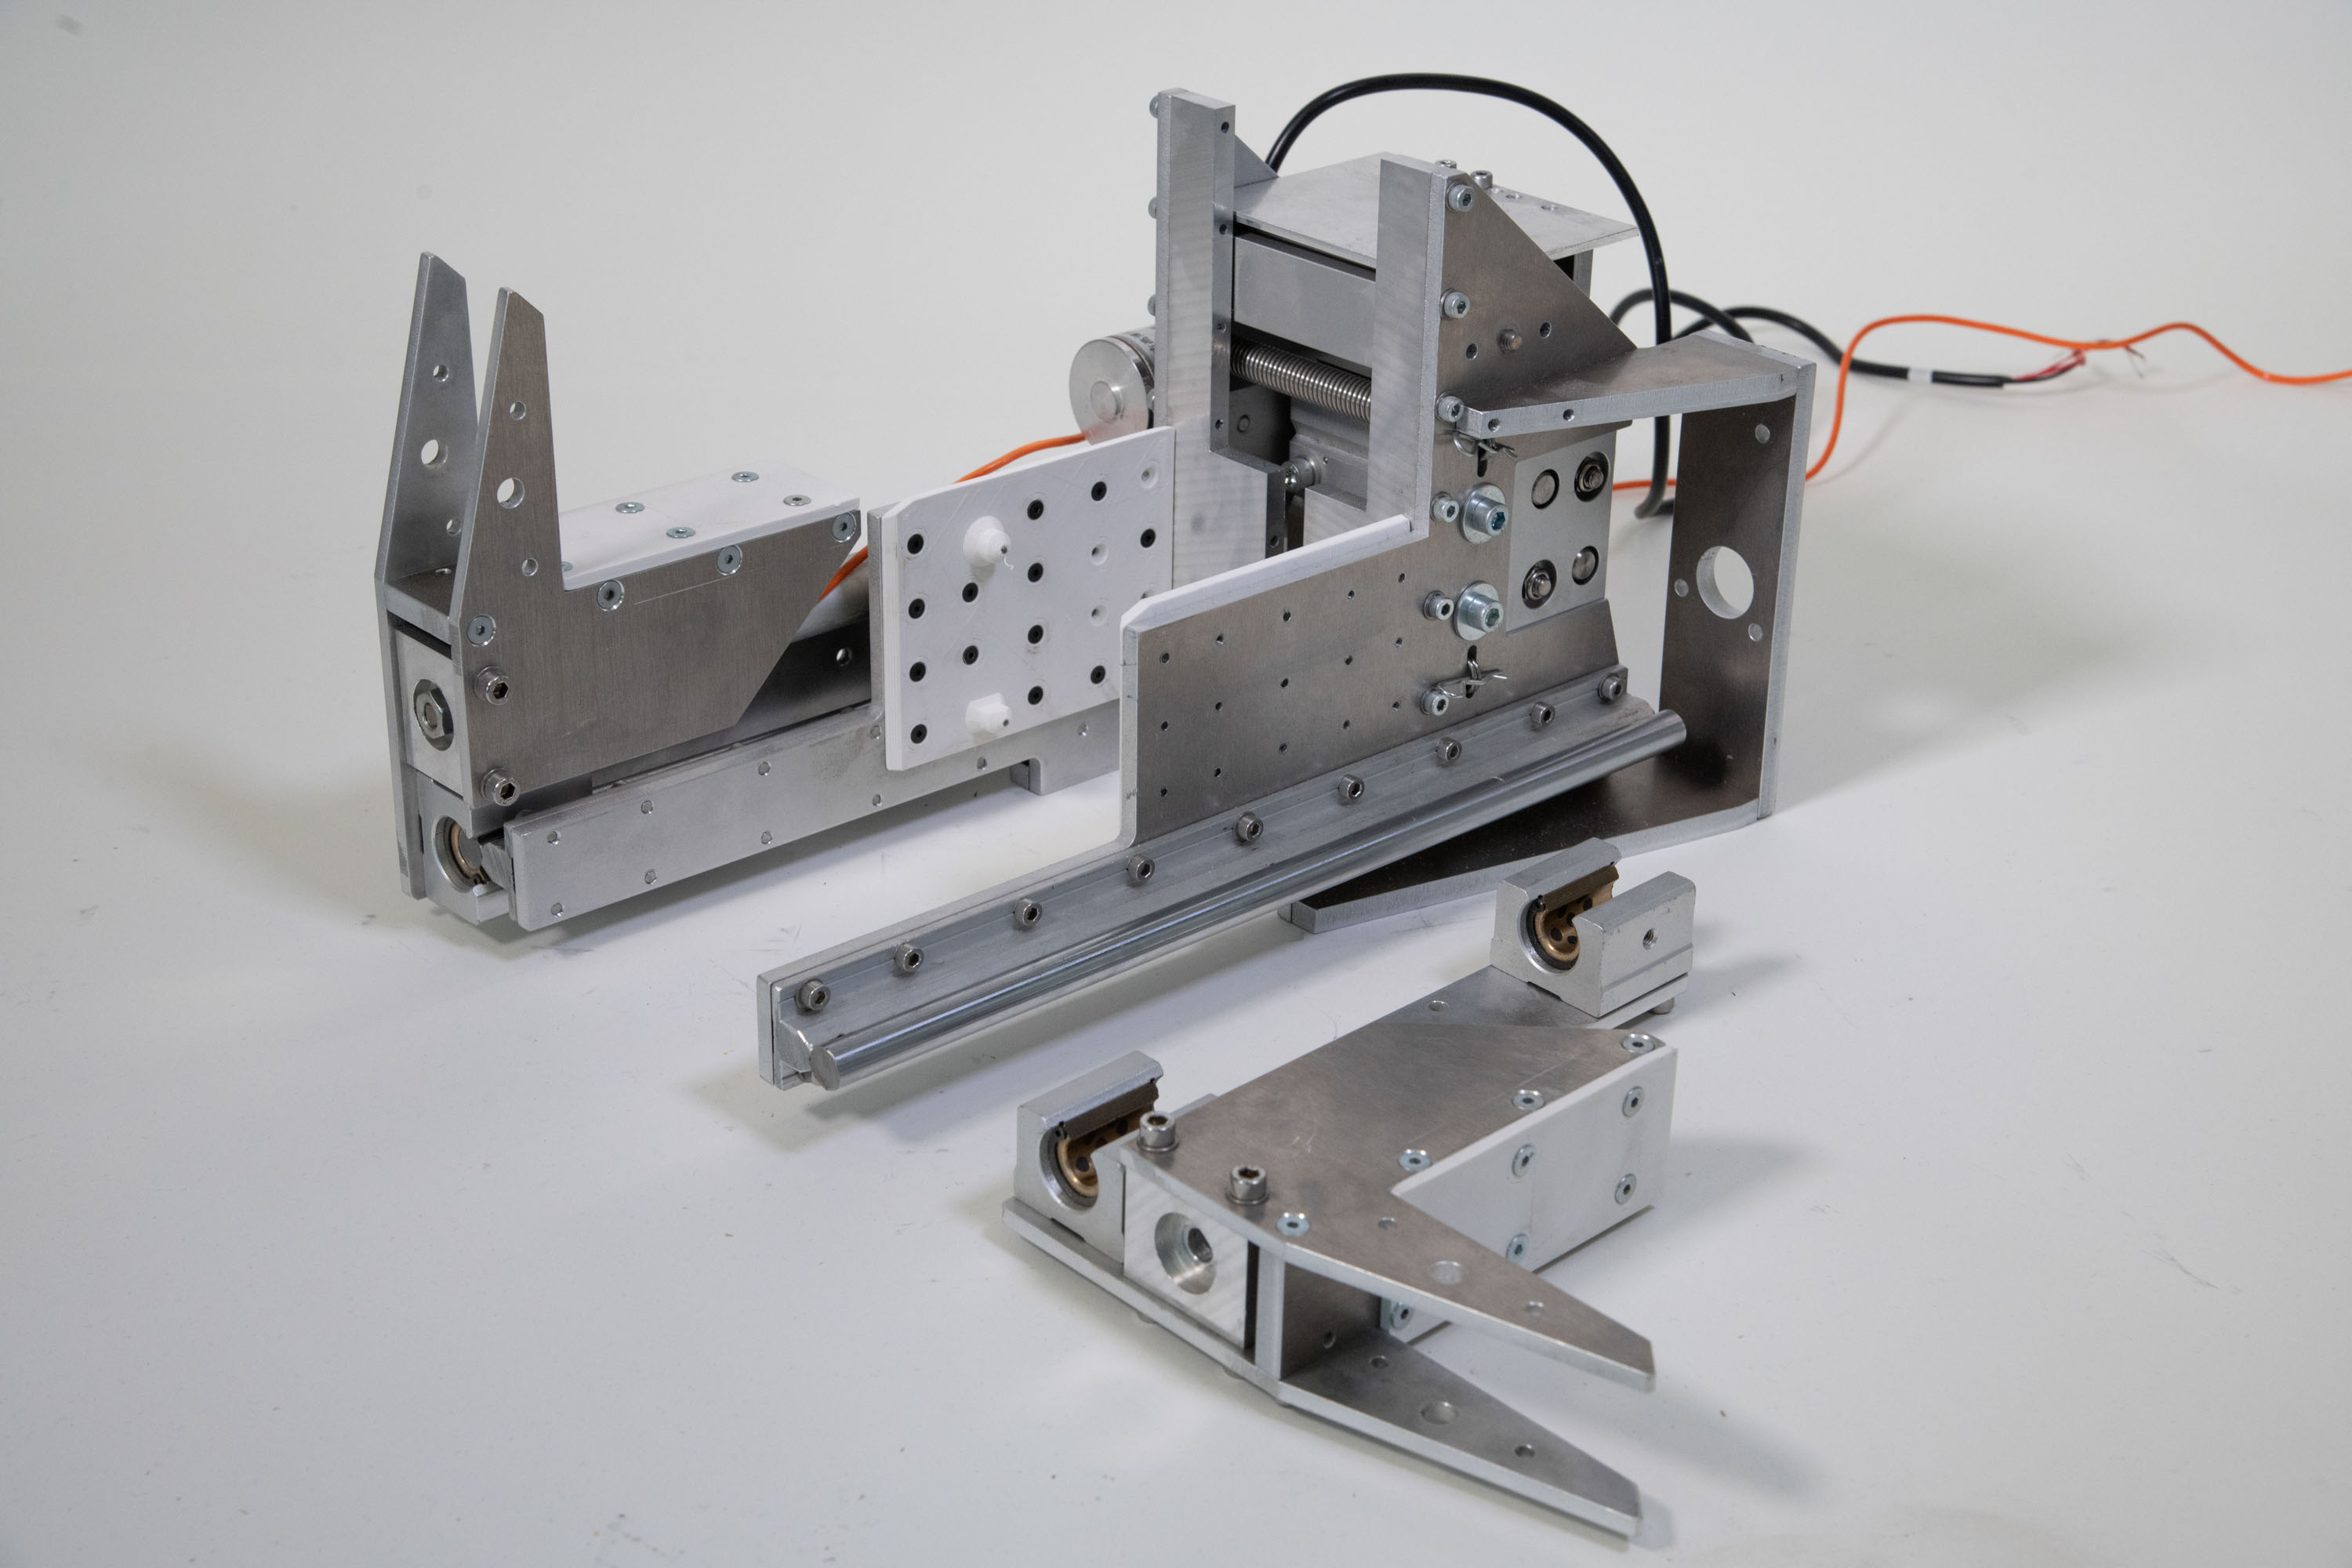
\includegraphics[width=0.99\textwidth]{images/04-4+5/cl1-broken-jaw.jpg}
    \caption{CL1 clamp jaw with two round bushings}
    \label{fig:cl1-broken-jaw-photo}
\end{figure}

\paragraph{Possible Solution and Follow-Up}

\begin{itemize}[nosep]
    \item Use an extra linear guide rail on each jaw.
    \begin{itemize}
        \item This is likely to be bulky and can further increase weight
    \end{itemize}
    \item Use linear guide rails with square or rectangular profiles with recirculating ball bearings.
    \begin{itemize}
        \item These guides are capable of resisting rotation with a single rail but their load ratings are also relatively low due to the small contact surface area over the balls. However their popularity and low cost offered by generic brands justified a test in Exploration Round 2 \seeref{subsection:exploration-2-ball-screw-linear-actuator}
    \end{itemize}
\end{itemize}
        
\subsection{Beam Support Needed During Clamping}
\label{subsection:exploration-1-beam-support-needed-during-clamping}

To further elaborate the problem observed before \seeref{subsection:exploration-1-successful-validation}, the clamp jaw was able to support the moving beam only in a horizontal position. However, the DiRT assembly system was envisioned to be able to assemble columns, beams and diagonal bracings. Therefore it would be necessary for the moving beam to be stable in other orientations too.

\paragraph{Possible Solution and Follow-Up}

The most obvious solution to this issue was to use the robotic arm to support the weight of the moving beam. Since the robotic arm was designed to transfer the timber beam to the clamps, it simply has to keep holding it while it moves. The beam gripper would then release the beam after the joints are securely clamped. 

On the positive side, it is a solution with very little or no additional hardware requirements, therefore it is easy to implement from the hardware perspective. The design of clamps can be also simplified because it no longer has to support the beam, making them easier to build and lighter weight. However, the worrying concern was that the movement of the robot and the clamps will have to be synchronised. This is known to be possible in industrial settings where external axes are integrated with the robot arm’s motion controller. However, synchronising it with an experimental remote-controlled device has no precedence and the programming and control implementation is likely to be challenging.

After trying to find alternative solutions with no avail, my decision was to pursue the synchronisation and control problem. A revised working hypothesis was created and tested in the next Exploration Round 2 \seeref{subsection:exploration-2-synchronisation-between-clamp-and-rfl-robot}. This pursuit would eventually lead to the discovery of many technical problems that were rarely discussed in the field of digital fabrication. Nevertheless, the Clamp and Arm synchronised Motion would be solved in Exploration Round 4 and 5.

\subsection{Design Study using Orthogonal Lap Joint}
\label{subsection:exploration-1-design-study-using-orthogonal-lap-joint}

% 2 x 2 Images
\begin{figure}[p]
    \centering
    \begin{subfigure}[b]{0.49\textwidth}
        \centering
        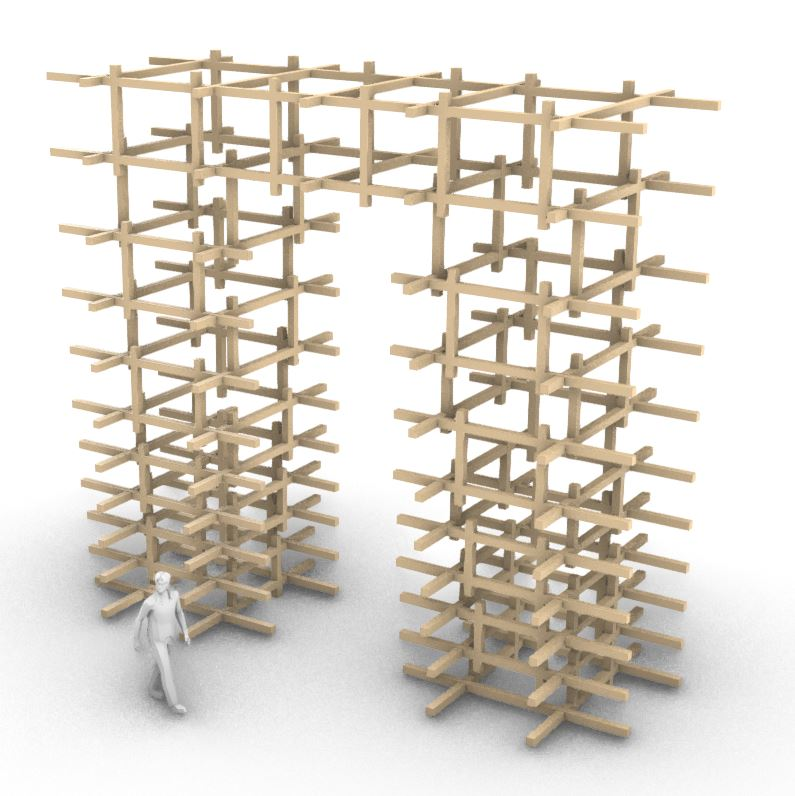
\includegraphics[width=\textwidth]{images/04-4+5/ortho-design-study2.jpg}
        % \caption{SubFigureCaption}
        %\label{fig:uniquesubfigurelabel}
    \end{subfigure}
    \hfill
    \begin{subfigure}[b]{0.49\textwidth}
        \centering
        \includegraphics[width=\textwidth]{images/04-4+5/ortho-design-study1.jpg}
        % \caption{SubFigureCaption}
        %\label{fig:uniquesubfigurelabel}
    \end{subfigure}
    \vskip\baselineskip % Next row
    \begin{subfigure}[b]{0.49\textwidth}
        \centering
        \includegraphics[width=\textwidth]{images/04-4+5/ortho-design-study3.jpg}
        % \caption{SubFigureCaption}
        %\label{fig:uniquesubfigurelabel}
    \end{subfigure}
    \hfill
    \begin{subfigure}[b]{0.49\textwidth}
        \centering
        \includegraphics[width=\textwidth]{images/04-4+5/ortho-design-study4.jpg}
        % \caption{SubFigureCaption}
        %\label{fig:uniquesubfigurelabel}
    \end{subfigure}
    \caption{Design study using orthogonal lap joints}
    \label{fig:design-study-ortho-lap-joint}
\end{figure}


A design study was conducted to determine if it is possible to create a demonstrator structure with only orthogonal lap joints. The intention is to understand whether the limitation of the CL3 Clamp is acceptable for creating convincing demonstration. Figure \ref{fig:design-study-ortho-lap-joint} shows some of the design sketches.  

\todo{Following paragraph is rephrased}
Throughout the design exercise, I found that it is very limiting to use only orthogonal joints. It was not possible to create triangulation for structural stability or to create an angled roof. The lower right option in Figure \ref{fig:design-study-ortho-lap-joint} where the joints are oriented differently is perhaps the most visually interesting. However these designs remain very sculptural due to the inability to create a structurally strong enclosure with architectural relevance. Nevertheless, this design exercise served to inform the development in the next round \seeref{section:exploration-2-goal} to prioritise redesigning the clamp to handle non-orthogonal lap joints.
